\documentclass[12pt,letterpaper,openany]{book}
\usepackage{subcaption}
\usepackage{enumerate} 
\usepackage{amsmath}
\usepackage{amsfonts}
\usepackage{amssymb}
\usepackage{booktabs}
\usepackage[utf8]{inputenc}
\usepackage[spanish,es-tabla]{babel}
\usepackage[left=3 cm,right=3 cm,bottom=2.5 cm,top=2.5 cm]{geometry}
\usepackage{graphicx}
\usepackage{cite}
\usepackage{hyperref}
\usepackage{tocloft}
\newcommand{\grad}{$^{\circ}$}
\usepackage{float}
\usepackage{colortbl}
\usepackage[dvipsnames,table,xcdraw]{xcolor}
\date{}
\setcounter{secnumdepth}{3} % para que ponga 1.1.1.1 en subsubsecciones
\setcounter{tocdepth}{3} % para que ponga subsubsecciones en el indice
\usepackage{fancyhdr}
\pagestyle{fancy}
\raggedbottom
\begin{document}
\fancyhead[RO,LE]{}

%%%%%%%%%%%%%%%%%%%%%%%%%%%%%%%%%%%%%%%%%%%%%%%%%%%%%%%%%%%%%%%%%%%%%%%%%%%%%%%%%%%%%%%%%%
%%%%%%%%%%%%%%%%%%%%%%%%%%%%%%						PORTADA
%%%%%%%%%%%%%%%%%%%%%%%%%%%%%%%%%%%%%%%%%%%%%%%%%%%%%%%%%%%%%%%%%%%%%%%%%%%%%%%%%%%%%%%%%%
\begin{titlepage}

%Primera portada
\begin{center}

\begin{figure}[htb]
\begin{center}

\includegraphics[width=5cm]{./imagenes/logo}
\end{center}
\end{figure}

\textbf{SISTEMA DE RECOMENDACIÓN DE SITIOS TURÍSTICOS Y COMERCIO PARA EL MUNICIPIO DE GINEBRA (VALLE)} \\

\vspace*{1.5in}
ANDRÉS FELIPE MEDINA TASCÓN \footnote{andres.medina@correounivalle.edu.co}\\
OSCAR ALEXANDER RUIZ PALACIO \footnote{ruiz.oscar@correounivalle.edu.co}\\

\vspace*{1.5in}
UNIVERSIDAD DEL VALLE\\
FACULTAD DE INGENIERÍA\\
ESCUELA DE INGENIERÍA DE SISTEMAS Y CIENCIAS DE LA COMPUTACIÓN\\
INGENIERÍA DE SISTEMAS\\
TULUÁ
2019

\end{center}
%Fin Primera portada

%Segunda portada
\vspace*{1.6in}
\begin{center}

\begin{figure}[htb]
\begin{center}

\includegraphics[width=5cm]{./imagenes/logo}
\end{center}
\end{figure}

\textbf{SISTEMA DE RECOMENDACIÓN DE SITIOS TURÍSTICOS Y COMERCIO PARA EL MUNICIPIO DE GINEBRA (VALLE)} \\

\vspace*{1.3in}
TRABAJO DE GRADO PRESENTADO COMO REQUISITO PARA OPTAR POR EL TÍTULO DE INGENIERO DE SISTEMAS \\

\vspace*{1.3in}
DIRECTOR DE TRABAJO DE GRADO \\
ING. ROYER DAVID ESTRADA ESPONDA. MS. C. \footnote{royer.estrada@correounivalle.edu.co}\\

\vspace*{1.3in}
UNIVERSIDAD DEL VALLE\\
FACULTAD DE INGENIERÍA\\
ESCUELA DE INGENIERÍA DE SISTEMAS Y CIENCIAS DE LA COMPUTACIÓN\\
INGENIERÍA DE SISTEMAS\\
TULUÁ
2019

\end{center}
%Fin Segunda portada
\thispagestyle{empty}
\end{titlepage}
%%%%%%%%%%%%%%%%%%%%%%%%%%%%%%%%%%%%%%%%%%%%%%%%%%%%%%%%%%%%%%%%%%%%%%%%%%%%%%%%%%%%%%%%%%
%%%%%%%%%%%%%%%%%%%%%%%%%%%%%%						FIN PORTADA
%%%%%%%%%%%%%%%%%%%%%%%%%%%%%%%%%%%%%%%%%%%%%%%%%%%%%%%%%%%%%%%%%%%%%%%%%%%%%%%%%%%%%%%%%%

%%%%%%%%%%%%%%%%%%%%%%%%%%%%%%%%%%%%%%%%%%%%%%%%%%%%%%%%%%%%%%%%%%%%%%%%%%%%%%%%%%%%%%%%%%
%%%%%%%%%%%%%%%%%%%%%%%%%%%%%%						NOTA DE ACEPTACION	
%%%%%%%%%%%%%%%%%%%%%%%%%%%%%%%%%%%%%%%%%%%%%%%%%%%%%%%%%%%%%%%%%%%%%%%%%%%%%%%%%%%%%%%%%%
\chapter*{Nota de Aceptación}
\pagenumbering{Roman} % para comenzar la numeracion de paginas en numeros romanos
\vspace*{1in}
\begin{center}
\rule{90mm}{0.1mm} \newline
\rule{90mm}{0.1mm} \newline
\rule{90mm}{0.1mm} \newline
\rule{90mm}{0.1mm} \newline
\end{center}

\vspace*{1.5in}
\rule{90mm}{0.1mm} \newline
Ing. Royer David Estrada Esponda. Ms. C. \\
Director

\vspace*{1.3in}
\rule{60mm}{0.1mm} \hfill \rule{60mm}{0.1mm} \newline
Jurado 1 \hfill Jurado 2
%%%%%%%%%%%%%%%%%%%%%%%%%%%%%%%%%%%%%%%%%%%%%%%%%%%%%%%%%%%%%%%%%%%%%%%%%%%%%%%%%%%%%%%%%%
%%%%%%%%%%%%%%%%%%%%%%%%%%%%%%						FIN NOTA DE ACEPTACION	
%%%%%%%%%%%%%%%%%%%%%%%%%%%%%%%%%%%%%%%%%%%%%%%%%%%%%%%%%%%%%%%%%%%%%%%%%%%%%%%%%%%%%%%%%%

%%%%%%%%%%%%%%%%%%%%%%%%%%%%%%%%%%%%%%%%%%%%%%%%%%%%%%%%%%%%%%%%%%%%%%%%%%%%%%%%%%%%%%%%%%
%%%%%%%%%%%%%%%%%%%%%%%%%%%%%%						DEDICATORIAS
%%%%%%%%%%%%%%%%%%%%%%%%%%%%%%%%%%%%%%%%%%%%%%%%%%%%%%%%%%%%%%%%%%%%%%%%%%%%%%%%%%%%%%%%%%
\chapter*{Dedicatorias}
\addcontentsline{toc}{chapter}{Dedicatorias} % si queremos que aparezca en el índice
\begin{flushright}
\textit{Aquí iria una dedicatoria \\
si tuviera una}
\end{flushright}
%%%%%%%%%%%%%%%%%%%%%%%%%%%%%%%%%%%%%%%%%%%%%%%%%%%%%%%%%%%%%%%%%%%%%%%%%%%%%%%%%%%%%%%%%%
%%%%%%%%%%%%%%%%%%%%%%%%%%%%%%						FIN DEDICATORIAS
%%%%%%%%%%%%%%%%%%%%%%%%%%%%%%%%%%%%%%%%%%%%%%%%%%%%%%%%%%%%%%%%%%%%%%%%%%%%%%%%%%%%%%%%%%

%%%%%%%%%%%%%%%%%%%%%%%%%%%%%%%%%%%%%%%%%%%%%%%%%%%%%%%%%%%%%%%%%%%%%%%%%%%%%%%%%%%%%%%%%%
%%%%%%%%%%%%%%%%%%%%%%%%%%%%%%						AGRADECIMIENTOS
%%%%%%%%%%%%%%%%%%%%%%%%%%%%%%%%%%%%%%%%%%%%%%%%%%%%%%%%%%%%%%%%%%%%%%%%%%%%%%%%%%%%%%%%%%
\chapter*{Agradecimientos} % si no queremos que añada la palabra "Capitulo"
\addcontentsline{toc}{chapter}{Agradecimientos} % si queremos que aparezca en el índice
\markboth{AGRADECIMIENTOS}{AGRADECIMIENTOS} % encabezado 
Royer David Estrada.\\
Joshua David Triana. \\

%%%%%%%%%%%%%%%%%%%%%%%%%%%%%%%%%%%%%%%%%%%%%%%%%%%%%%%%%%%%%%%%%%%%%%%%%%%%%%%%%%%%%%%%%%
%%%%%%%%%%%%%%%%%%%%%%%%%%%%%%						FIN AGRADECIMIENTOS
%%%%%%%%%%%%%%%%%%%%%%%%%%%%%%%%%%%%%%%%%%%%%%%%%%%%%%%%%%%%%%%%%%%%%%%%%%%%%%%%%%%%%%%%%%
 % para empezar la numeración con números
\newpage
\pagenumbering{arabic}
%%%%%%%%%%%%%%%%%%%%%%%%%%%%%%%%%%%%%%%%%%%%%%%%%%%%%%%%%%%%%%%%%%%%%%%%%%%%%%%%%%%%%%%%%%
%%%%%%%%%%%%%%%%%%%%%%%%%%%%%%						INDICES
%%%%%%%%%%%%%%%%%%%%%%%%%%%%%%%%%%%%%%%%%%%%%%%%%%%%%%%%%%%%%%%%%%%%%%%%%%%%%%%%%%%%%%%%%%
\tableofcontents % indice de contenidos

\newpage
\listoffigures % indice de figuras

\newpage
\listoftables % indice de tablas
%%%%%%%%%%%%%%%%%%%%%%%%%%%%%%%%%%%%%%%%%%%%%%%%%%%%%%%%%%%%%%%%%%%%%%%%%%%%%%%%%%%%%%%%%%
%%%%%%%%%%%%%%%%%%%%%%%%%%%%%%						FIN INDICES
%%%%%%%%%%%%%%%%%%%%%%%%%%%%%%%%%%%%%%%%%%%%%%%%%%%%%%%%%%%%%%%%%%%%%%%%%%%%%%%%%%%%%%%%%%

%%%%%%%%%%%%%%%%%%%%%%%%%%%%%%%%%%%%%%%%%%%%%%%%%%%%%%%%%%%%%%%%%%%%%%%%%%%%%%%%%%%%%%%%%%
%%%%%%%%%%%%%%%%%%%%%%%%%%%%%%					 RESUMEN
%%%%%%%%%%%%%%%%%%%%%%%%%%%%%%%%%%%%%%%%%%%%%%%%%%%%%%%%%%%%%%%%%%%%%%%%%%%%%%%%%%%%%%%%%%
\chapter*{Resumen} % si no queremos que añada la palabra "Capitulo"
\addcontentsline{toc}{chapter}{Resumen} % si queremos que aparezca en el índice
El municipio de Ginebra, ubicado en el Valle del Cauca, cuenta con una cantidad considerable de turistas cada fin de semana y festividades, lo que hace que el turismo sea uno de los grandes atractivos que posee el municipio, siendo un destino gastronómico, cultural y natural. Con este proyecto se quiere lograr dar mayor visibilidad a toda la variedad de destinos que tiene el municipio mediante un sistema de recomendación incorporado en una aplicación móvil para que las personas, tanto locales y turistas, tengan la posibilidad de ver todos los sitios disponibles, calificarlos y recibir recomendaciones automatizadas.\\
En el presente documento se expone la manera de llevar a cabo el desarrollo de esta aplicación móvil, como también la implementación del sistema de recomendación y su funcionamiento, además de la revisión literaria que se usó como fuente de apoyo, y los demás componentes de desarrollo utilizados en el transcurso del proyecto.
\vspace{5mm}\newline
\textbf{Palabras claves:} Aplicación Móvil, Ginebra, Sistema de Recomendación, Turismo.

%%%%%%%%%%%%%%%%%%%%%%%%%%%%%%%%%%%%%%%%%%%%%%%%%%%%%%%%%%%%%%%%%%%%%%%%%%%%%%%%%%%%%%%%%%
%%%%%%%%%%%%%%%%%%%%%%%%%%%%%%						FIN RESUMEN
%%%%%%%%%%%%%%%%%%%%%%%%%%%%%%%%%%%%%%%%%%%%%%%%%%%%%%%%%%%%%%%%%%%%%%%%%%%%%%%%%%%%%%%%%%

%%%%%%%%%%%%%%%%%%%%%%%%%%%%%%%%%%%%%%%%%%%%%%%%%%%%%%%%%%%%%%%%%%%%%%%%%%%%%%%%%%%%%%%%%%
%%%%%%%%%%%%%%%%%%%%%%%%%%%%%%						INTRODUCCION
%%%%%%%%%%%%%%%%%%%%%%%%%%%%%%%%%%%%%%%%%%%%%%%%%%%%%%%%%%%%%%%%%%%%%%%%%%%%%%%%%%%%%%%%%%
\chapter{Introducción}\label{cap.introduccion}
Los sistemas de recomendación son herramientas que ofrecen sugerencias útiles a las personas, siendo muy utilizados en el ámbito de entretenimiento, por otro lado, el significativo crecimiento en los últimos años que ha tenido la comercialización de dispositivos móviles y por consiguiente las aplicaciones que en ellos se instalan, ha provocado un notable incremento en la adquisición y su uso por parte de las personas, permitiendo el acceso de información en cualquier lugar y momento, creando la necesidad de desarrollar aplicaciones móviles que satisfagan necesidades asociadas a entretenimiento, viajes y turismo.
\vspace{5mm}\newline
El uso de los sistemas de recomendación se está contemplando cada vez más debido a que son muy útiles al momento de evaluar y filtrar la gran cantidad de información disponible con objeto de asistir a los usuarios en sus procesos de exploración y de búsqueda\cite{1}. Por otro lado, una aplicación móvil permite a las personas que interactúan con ella, a efectuar una tarea concreta de cualquier tipo, facilitando las gestiones o actividades a desarrollar\cite{2}.
\vspace{5mm}\newline
Teniendo en cuenta que el turismo es considerado como actividad económica de gran importancia, la cual representa un potencial enorme de desarrollo y progreso, el desarrollo de este proyecto se basa en la utilidad que representa hoy en día el uso de las aplicaciones móviles y los sistemas de recomendación, facilitando la exploración de los diferentes sitios y lugares de interés dentro del municipio.

\section{Descripción del Problema}
Hoy en día el municipio de Ginebra es reconocido por sus populares festividades y más visitantes recorren el municipio con más frecuencia, según la alcaldía de Ginebra en el año 2000, el municipio presentaba una cifra de aproximadamente 600 turistas al día durante los fines de semana y días festivos\cite{3}. También se ha visto un incremento de la población lo que ha generado una expansión dentro de su zona urbana y en sus corregimientos, el gobierno actual de Ginebra informa que actualmente se construyen 74 viviendas\cite{4} anualmente lo que conlleva a un crecimiento en el comercio del municipio. Diferentes aplicaciones como Google Maps indican sitios de interés del municipio, pero su precisión se enfrenta a una desactualización con respecto a la reciente expansión, esto genera que los turistas y locales se encuentren ante un problema al momento de decidir un lugar para poder realizar una actividad específica. Para elegir estos lugares se basan en recomendaciones de otras personas o simplemente escogen un lugar intuitivamente para lo que deseen hacer. 
\vspace{5mm}\newline
Una de las desventajas para la promoción de nuevos sitios por conocer en el municipio, es que el visitante tiene como punto de referencia los lugares con más tradición en el mismo, dejando a un lado la oportunidad de explorar sitios nuevos los cuales puedan ser de su interés.
\vspace{5mm}\newline
Considerando el flujo de personas que actualmente visitan el municipio de Ginebra para realizar sus actividades de descanso y esparcimiento, el desarrollo de las nuevas tecnologías de la información y comunicación permiten promover a mayor escala el turismo a través de los sistemas de recomendación y las aplicaciones móviles.
\vspace{5mm}\newline
Teniendo en cuenta el gran uso de estos sistemas en las aplicaciones\cite{5}, cobra importancia desarrollar un prototipo de una aplicación móvil de un sistema de recomendación para que los habitantes y turistas del municipio de Ginebra tengan a su disposición una visión, descripción, opiniones e información sobre los establecimientos, sitios de interés y eventos a los cuales puedan acudir, permitiendo la interacción entre usuarios y comerciantes en tiempo real.

\section{Formulación del Problema}
¿Cómo promover el turismo del municipio de Ginebra por medio de un sistema de recomendación que pueda ser usado desde dispositivos móviles?

\section{Objetivos}
\subsection{Objetivo General}
Desarrollar un prototipo de sistema de recomendación que pueda ser usado por medio de dispositivos móviles para promover el turismo en el municipio de Ginebra
\subsection{Objetivos Específicos}
\begin{enumerate}
    \item Caracterizar los sitios y eventos del municipio de Ginebra.
    \item Determinar el tipo de sistema de recomendación y los algoritmos a utilizar.
    \item Implementar un prototipo de una aplicación móvil que permita consumir y ofrecer la información sobre los sitios y eventos de la ciudad de Ginebra.
    \item Implementar un prototipo de sistema de recomendación para los sitios y eventos del municipio de Ginebra.
    \item Evaluar las recomendaciones emitidas por el sistema de recomendación conforme a la realimentación de los usuarios de la aplicación.
\end{enumerate}

\section{Estructura del Documento}
El presente documento se compone de 4 capítulos en donde el primero de ellos concluye en este punto después de citar aspectos generales, objetivos y alcance del proyecto. El capitulo 2 denominado Marco de referencia reúne aportes teóricos, conceptuales y un grupo de antecedentes que tienen como objetivo contextualizar al lector en relación al tema principal de este proyecto, por otro lado, el capitulo 3 describe el proceso de ingeniería de software llevado a cabo para el desarrollo del proyecto, así como también expone brevemente la metodología usada, los artefactos utilizados y las pruebas realizadas; entre otros elementos. Por último, el capitulo 4 expone las conclusiones y trabajos futuros que podrían presentarse.
%%%%%%%%%%%%%%%%%%%%%%%%%%%%%%%%%%%%%%%%%%%%%%%%%%%%%%%%%%%%%%%%%%%%%%%%%%%%%%%%%%%%%%%%%%
%%%%%%%%%%%%%%%%%%%%%%%%%%%%%%						FIN INTRODUCCION
%%%%%%%%%%%%%%%%%%%%%%%%%%%%%%%%%%%%%%%%%%%%%%%%%%%%%%%%%%%%%%%%%%%%%%%%%%%%%%%%%%%%%%%%%%

%%%%%%%%%%%%%%%%%%%%%%%%%%%%%%%%%%%%%%%%%%%%%%%%%%%%%%%%%%%%%%%%%%%%%%%%%%%%%%%%%%%%%%%%%%%%%%%%%%
%%%%%%%%%%%%%%%%%%%%%%%%%%%%%%%%%%%%%%%%%%%%%%%%%%%%%%%%%%%%%%%%%%%%%%%%%%%%%%%%%%%%%%%%%%%%%%%%%%
%%%%%%%%%%%%%%%%%%%%%%%%%%%%%%%%%%%%%%%%%%%%%%%%%%%%%%%%%%%%%%%%%%%%%%%%%%%%%%%%%%%%%%%%%%%%%%%%%%
%%%%%%%%%%%%%%%%%%%%%%%%%%%%%%%%%%%%%%%%%%%%%%%%%%%%%%%%%%%%%%%%%%%%%%%%%%%%%%%%%%%%%%%%%%%%%%%%%%

%%%%%%%%%%%%%%%%%%%%%%%%%%%%%%%%%%%%%%%%%%%%%%%%%%%%%%%%%%%%%%%%%%%%%%%%%%%%%%%%%%%%%%%%%%
%%%%%%%%%%%%%%%%%%%%%%%%%%%%%%						MARCO DE REFERENCIA
%%%%%%%%%%%%%%%%%%%%%%%%%%%%%%%%%%%%%%%%%%%%%%%%%%%%%%%%%%%%%%%%%%%%%%%%%%%%%%%%%%%%%%%%%%
\chapter{Marco de Referencia}\label{cap.marco_de_referencia}

\section{Marco Teórico}
\subsection{Gestión Turística}
La industria del turismo es considerada una de las maneras más productivas para obtener recursos para un país o región, convirtiéndose en uno de los sectores de la economía de más amplio crecimiento en la actualidad. En Colombia, el año 2017 fue muy positivo para el turismo, al punto de convertirse en el segundo generador de divisas del país, superando productos tradicionales como el café, las flores y el banano. Según Migración Colombia, durante el año pasado ingresaron al país un total de 3’344.382 viajeros, lo que representa un crecimiento de casi 20\% con respecto al 2016\cite{6}.
\vspace{5mm}\newline
El turismo promueve viajes de todo tipo: con fines de descanso, motivos culturales, interés social, negocios o simplemente ocio. El fuerte desarrollo experimentado por el turismo cultural en los últimos años, se enmarca en los cambios acaecidos en los destinos turísticos antes los procesos de diversificación y especialización de la demanda, que obligan a estos espacios a una búsqueda constante de singularización y diferenciación de sus productos que atiendan a este consumo individualizado\cite{7}.
\vspace{5mm}\newline
Posee todas las características de un mercado, en él se hallan dos elementos que conforman la producción. El primero es la oferta turística y el segundo es el consumo, es decir, la demanda, la cual se da de manera conjunta entre bienes y servicios. Esta industria básicamente está compuesta por el hombre, que es el elemento subjetivo, y por el equipamiento turístico que es el elemento objetivo, para que estos elementos logren constituir el consumo turístico, debe darse una relación directa entre ellos\cite{8}. 

\subsection{Gestión Turística y las TIC}
Las TIC son todos aquellos recursos, herramientas o programas que se utilizan para el procesamiento y el compartir información mediante diversos medios tecnológicos, siendo actualmente la herramienta vital para la difusión de información.
El uso de las TIC permite obtener fácilmente información referente a productos de nuestro interés, siendo altamente utilizada por los profesionales dentro del ámbito del turismo, para su promoción.
\vspace{5mm}\newline
Las TIC han permitido llevar la globalidad del mundo de la comunicación, facilitando la interconexión entre las personas e instituciones a nivel mundial, y eliminando barreras espaciales y temporales. 
\vspace{5mm}\newline
\textit{"El uso intensivo por parte del turista de las Nuevas Tecnologías de la Información y las Comunicaciones (NTIC), tanto en la organización como en el desarrollo del viaje, han revolucionado la forma de promocionar un territorio turístico ya que, cualquier destino que pretenda ser competitivo debe actualizar continuamente toda aquella información que pueda ser de interés para el visitante (localización e interpretación de los recursos, horarios de equipamientos y servicios, etc.), especialmente si este pertenece al segmento del turismo cultural, tipología de usuario que demanda gran cantidad de información sobre los recursos de un destino y cuya motivación principal es el disfrute de los bienes culturales.
Este turista, consumidor de TIC, se ha transformando en un usuario 2.0, caracterizado por estar altamente conectado y, por tanto, hacer un uso constante de la red mediante su dispositivo móvil, junto a esto ha pasado de ser un mero visualizador a un generador de información en redes sociales, blogs, etc., y colabora de forma activa aportando su opinión sobre el destino mediante los sistemas de reputación on-line. En consecuencia, surge el turista 2.0, que requiere de información del territorio turístico, en el proceso de anticipación (promoción y marketing), experiencia (comunicación) y recreación (búsqueda de más información, publicaciones y recomendaciones) del viaje turístico.”} \cite{9}.

\subsection{Dispositivos Móviles}
Un dispositivo móvil se puede definir como un aparato de pequeño tamaño, con algunas capacidades de procesamiento, con conexión permanente o intermitente a una red, con memoria limitada, que ha sido diseñado específicamente para una función, pero que puede llevar a cabo otras funciones más generales\cite{10}.
\vspace{5mm}\newline
En los últimos años, se ha podido observar un gran crecimiento en el desarrollo de dispositivos móviles, algunos de estos dispositivos son los reproductores de audio portátiles (Desde el walkman hasta los reproductores digitales mp3, mp4, etc.), navegadores GPS, teléfonos móviles, teléfonos inteligentes (Smartphone), PDAs (Asistente digital de persona) o los Tablet PCs.
\vspace{5mm}\newline
Es muy visto cómo los teléfonos móviles son los dispositivos que más impacto tienen dentro del mercado, debido a la gran variedad que existen y a la mayor evolución que presenta comparado con otros dispositivos móviles, es por esto que \textit{"hoy en día es cada vez más frecuente utilizar dispositivos móviles, Smartphone o Tabletas, como herramientas de trabajo, éstos dispositivos día tras día aumentan en prestaciones y en posibilidades de uso, por lo que estos se están convirtiendo en herramientas fundamentales para trabajar en movilidad e incluso, como sustitutos de los computadores para determinadas situaciones y tareas que los usuarios desean realizar.”} \cite{11} 

\subsubsection{Aplicaciones Móviles}
Se denomina aplicación móvil o app a toda aplicación informática diseñada para ser ejecutada en teléfonos inteligentes, tabletas y otros dispositivos móviles. Por lo general se encuentran disponibles a través de plataformas de distribución, operadas por las compañías propietarias de los sistemas operativos móviles como Android, iOS, BlackBerry OS y Windows Phone, entre otros\cite{2}.
\vspace{5mm}\newline
Actualmente, el fácil acceso que tienen las personas a un teléfono inteligente, ha hecho que en los últimos años el mercado de las aplicaciones móviles experimente una rápida expansión. Día a día se desarrollan nuevas aplicaciones que ofrecen cada vez más características que buscan satisfacer las diferentes necesidades de los usuarios, como también aplicaciones que brindan entretenimiento al usuario.
\vspace{5mm}\newline
Existen 3 tipos de enfoques para desarrollar aplicaciones móviles que se deben de tener en cuenta, ya que decidir usarlas y programarlas depende de diversos factores, como el objetivo para el cual va a ser creada, llegando a presentar una seria de ventajas o desventajas:
\vspace{5mm}\newline
\textbf{Aplicaciones Nativas}\newline
Son las aplicaciones que se desarrollan orientadas a un sistema operativo específico. Las aplicaciones nativas ofrecen una gran ventaja de permitir el acceso completo a todas las funcionalidades del dispositivo y visibilidad en las tiendas de aplicaciones del respectivo sistema operativo (Google Play, Apple App Store, Windows Store, etc.), ofreciendo una mejor experiencia de usuario.
\vspace{5mm}\newline
\textbf{Aplicaciones Híbridas}\newline
Son las aplicaciones que se desarrollan para que funcionen en varios Sistemas Operativos, como por ejemplo WhatsApp, Twitter, Instagram, etc. Estas aplicaciones están programadas con tecnologías WEB (HTML5, CSS, JS) y están distribuidas en las tiendas de aplicación.
Estas aplicaciones suelen ofrecer una peor experiencia de usuario, pero son más baratas de desarrollar.
\vspace{5mm}\newline
\textbf{Aplicaciones Web}\newline
Son aplicaciones que se ejecutan desde un servidor, se pueden usar en cualquier dispositivo que cuente con un navegador web y una de las ventajas que ofrece es que, al ser una página web, el usuario no tiene que estar descargando actualizaciones ya que accede directamente a la versión más actualizada o reciente.
Uno de los principales problemas de este tipo de aplicaciones es que se debe contar con una conexión de internet para poder hacer uso de esta, y al momento de desarrollarla, se debe tener presente las diferentes dimensiones de pantalla para que pueda ser visualizada de una manera correcta.

\subsubsection{Metodologías de desarrollo de aplicaciones móviles}
Una metodología es una colección de procedimientos, técnicas, herramientas y documentos auxiliares que ayudan a los desarrolladores de software en sus esfuerzos por implementar nuevos sistemas de información. Una metodología está formada por fases, cada una de las cuales se puede dividir en sub-fases, que guiarán a los desarrolladores de sistemas a elegir las técnicas más apropiadas en cada momento del proyecto y también a planificarlo, gestionarlo, controlarlo y evaluarlo.
\vspace{5mm}\newline
El uso de una metodología de desarrollo permite trabajar de una manera ordenada, con el fin de poder cumplir con todas las actividades y tareas establecidas en un tiempo limitado para el desarrollo de un software. 
\vspace{5mm}\newline
Las metodologías de desarrollo de software están clasificadas en 2 tipos de metodologías: las ágiles y las tradicionales. \cite{12} resume las características de ambas metodologías, en la siguiente tabla:

\begin{table}[H]
\centering
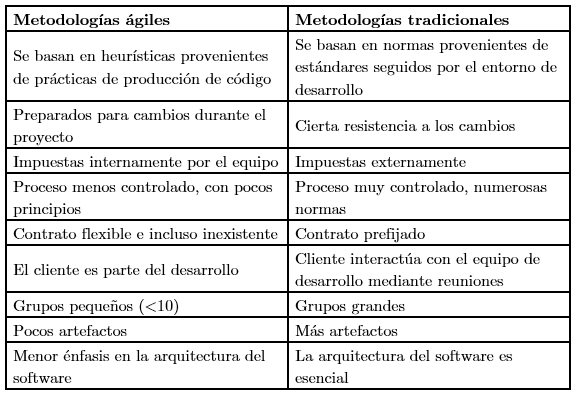
\includegraphics[width=13cm]{./imagenes/tablas/comparacion_metodologias}
\caption{Comparación de metodologías.}
\end{table}

El uso de una metodología ágil es una excelente alternativa para guiar proyectos de desarrollo de software de tamaño reducido, como es el caso de las aplicaciones móviles. 

\subsection{Sistemas recomendación}
Se puede definir los sistemas de recomendación como "el conjunto de herramientas de software y técnicas que ofrecen sugerencias útiles al usuario.” Hoy en día con el crecimiento que ha tenido internet en los últimos años y la creación de sitios que ofrecen servicios de todo tipo, ya sea para ver películas o escuchar música como son el caso de Netflix y Spotify, los usuarios muchas veces al tener tanta información y tal vez poca experiencia no saben que elegir y se dejan guiar por lo que digan otras personas, ya sea mediante conversaciones con personas conocidas, artículos de revistas, internet o la televisión.
\vspace{5mm}\newline
Los sistemas de recomendación se crean para que los usuarios tengan sugerencias personalizadas de acuerdo a sus gustos y preferencias, esto se realiza para que el usuario tenga una visión amplia de que puede explorar alternativas que le puedan gustar, los sitios webs para compras como Amazon utilizan estas técnicas para que todos los productos de calidad que ofrecen puedan ser visualizados por los usuarios de acuerdo a sus gustos y le pueda ser de utilidad a los usuarios. "Los sistemas de recomendación intentan predecir cuales son los productos o servicios más adecuados para el usuario de acuerdo a sus preferencias y restricciones".
\vspace{5mm}\newline
Los sistemas de recomendación son de gran utilidad tanto para los usuarios, como para los que la desarrollan. Para los usuarios, son muchos los motivos, uno de ellos es que puede encontrar una gran variedad de artículos y servicios que le sean de utilidad. Los desarrolladores de sistemas de recomendación han aumentado su interés en el desarrollo de sistemas para tiendas web, siendo una de las grandes motivaciones que presentan debido a que pueden obtener una mayor ganancia a través de la venta de una gran variedad de artículos que en muchas ocasiones puedan ser artículos difíciles de encontrar por parte de los usuarios. 
\vspace{5mm}\newline
A través de los sistemas de recomendación, los desarrolladores pueden entender lo que los usuarios están buscando, con el fin de satisfacer las necesidades de los usuarios e incrementando su fidelidad\cite{13}. 
\vspace{5mm}\newline
Los sistemas de recomendación tratan de predecir la calificación a un artículo o servicio determinado que los usuarios darían a partir de su información, ofreciendo una menor carga de información y conocimiento a través de la creación de un filtro y brindando información que pueda ser del interés que este aún no haya considerado\cite{6}. Esto lleva a que los sistemas de recomendación tengan ciertas particularidades dependiendo de las necesidades del usuario y las características del sistema. El manual de sistemas de recomendación\cite{13} proporciona una serie de características sobre estos sistemas, tales como el hallazgo de buenos artículos, colaboración por parte de otros usuarios, recomendaciones de secuencias o de paquetes.

\subsubsection{Técnicas de recomendación}
Existen una gran variedad de técnicas a la hora de realizar un sistema de recomendación el éxito o no de este dependen del diseño. Por lo cual es esencial tener en cuenta los usuarios, los ítems y las transacciones entre estos, por ejemplo, las calificaciones\cite{13}.
\vspace{5mm}\newline
\textbf{Filtro Colaborativo}\newline
Los sistemas de recomendación con filtro colaborativo es una de las técnicas más utilizadas a la hora de realizar sugerencias en aplicaciones con bastantes usuarios. Según Michael D. Ekstrand, John T. Riedl y Joseph A. Konstan \textit{"Es un algoritmo de recomendación popular que basa sus predicciones y recomendaciones en calificaciones o comportamientos de otros usuarios en el sistema"}\cite{14}. Para este proceso es necesario tener en cuenta la comunidad que forma parte del sistema tomando la retroalimentación que estos usuarios le dan con sus opiniones y calificaciones encontrando así características en común que puedan ser de utilidad para los usuarios\cite{15}.
Para el filtro colaborativo se tienen dos tipos esencialmente que son los que tienen información de los usuarios de forma explícita ya sea mediante las calificaciones que les dé a los artículos de su interés o ya que ingresa sus gustos directamente. Por otro lado, están los usuarios que no le otorgan tanta información al sistema de manera tan directa, es decir, se obtiene de manera implícita, de estos usuarios la información se toma por número de clics, historial de navegación, historial de compras en caso de e-commerce, son algunas de las maneras que se extrae información de estos a la hora de realizar recomendaciones\cite{13}.
\vspace{5mm}\newline
\textbf{Filtro Basado en Contenido}\newline
El filtro basado en contenido toma los ítems con su descripción y según el perfil de los usuarios determina cuales pueden ser de su interés, este proceso se realiza sobre todo en las aplicaciones en las cuales se hacen bastantes compras. "Las recomendaciones de estos sistemas depende de los artículos con los que el usuario ha interactuado. En particular, varios artículos candidatos se comparan con los artículos previamente calificados por el usuario y se recomiendan los artículos que mejor combinen.". \cite{13}, \cite{16}, \cite{17}.
\vspace{5mm}\newline
\textbf{Técnicas Híbridas}\newline
Estas técnicas de sistemas de recomendación se basan en la combinación de técnicas mencionadas anteriormente. Un sistema híbrido que combina las técnicas A y B, e intenta utilizar las ventajas de A para corregir las desventajas de B. Por ejemplo, los métodos de filtro colaborativo sufren problemas con nuevos ítems, es decir, no pueden recomendar artículos que no tienen calificaciones. Esto no tiene límites para el filtro basado en el contenido ya que la predicción para nuevos los artículos se basan en su descripción (características) que normalmente están disponibles\cite{13}. 

\subsubsection{Sistemas de recomendación para Turismo}
Según Michael J. Pazzani, \textit{"Los sistemas de recomendación existentes en el turismo electrónico obtienen la información del usuario, explícitamente (al preguntar) o implícitamente (extrayendo la actividad en línea del usuario), y sugerir destinos para visitar, puntos de interés, eventos / actividades o paquetes turísticos completos. El objetivo principal de los sistemas de recomendación para el turismo es facilitar el proceso de búsqueda de información para el viajero y convencerlo (persuadirlo) de la idoneidad de los servicios propuestos. En los últimos años, ha surgido una serie de sistemas de recomendación para el turismo y algunos de ellos ahora están operativos en los principales portales de turismo."}\cite{16}. 

\subsubsection{Sistemas de recomendación para Turismo en aplicaciones móviles}
Con el rápido desarrollo de las tecnologías móviles, varios tipos de aplicaciones móviles se han vuelto muy populares. Como tecnología revolucionaria, la informática móvil permite el acceso a la información en cualquier momento y en cualquier lugar, incluso en entornos con pocas conexiones de red. Entre otros, se ha estudiado activamente el uso efectivo de la tecnología móvil en el campo del turismo móvil. En esta línea, los sistemas de recomendación móviles (es decir sistemas de recomendación adaptados a las necesidades de los usuarios de dispositivos móviles) representan un hilo de investigación relativamente reciente con numerosos campos potenciales de aplicación  En particular, el turismo móvil es un campo de aplicación privilegiado para los sistemas de recomendación en dispositivos móviles, que aprovecha oportunidades masivas para proporcionar recomendaciones turísticas altamente precisas y efectivas que respeten las preferencias personales y capturen parámetros contextuales de uso, personales y ambientales\cite{16}. 

\subsection{Ginebra – Valle del Cauca}
\subsubsection{Aspectos Generales}
Según la alcaldía de Ginebra, \textit{"El Municipio de Ginebra se encuentra localizado en el piedemonte de la cordillera central, a 60 Km. de la ciudad de Santiago de Cali, capital del Departamento}.

\begin{figure}[H]
\begin{center}
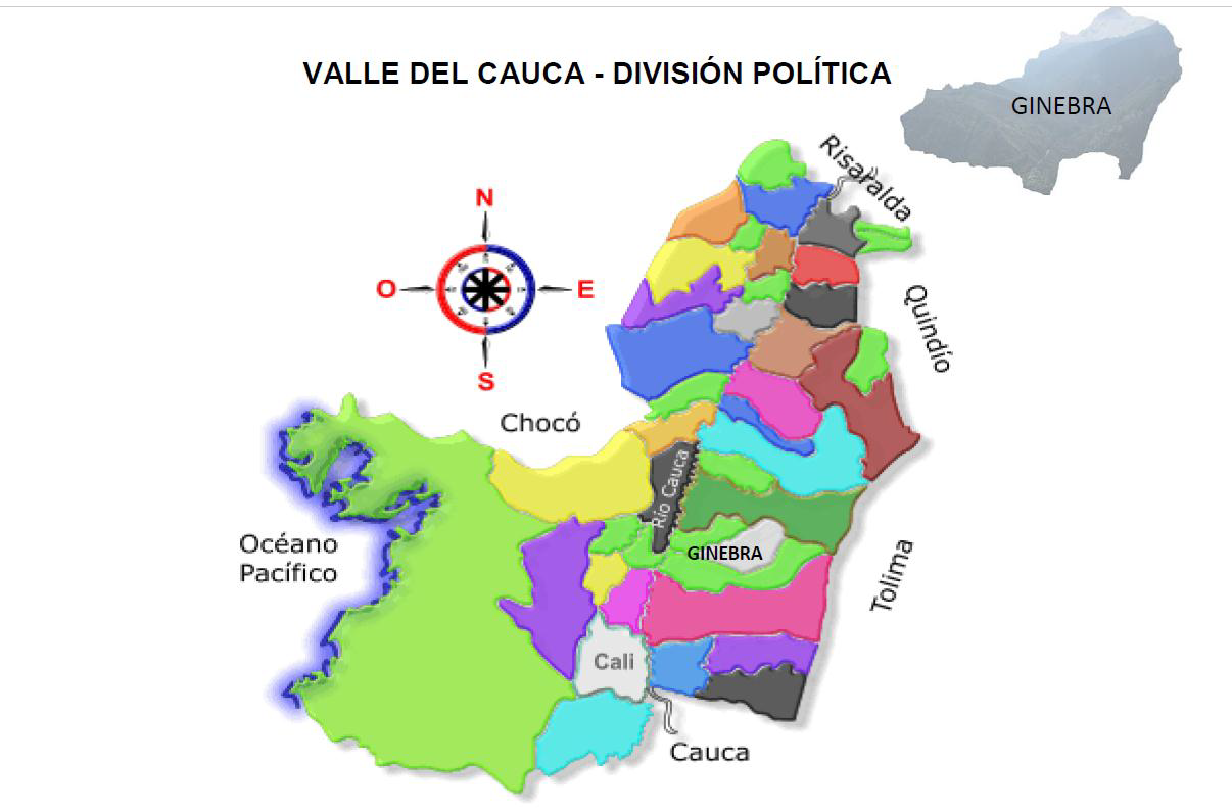
\includegraphics[width=10.7cm]{./imagenes/mapa_politico}
\caption{Mapa Político Valle del Cauca.}
\end{center}
\end{figure}

\textit{El municipio tiene un área aproximada de 24.674 ha, de las cuales corresponden al área urbana 29 ha y 24.645 ha al área rural. Cuenta con diferentes climas en la totalidad de su superficie desde cálido hasta páramo y su temperatura media es de 23 \grad C.}
\vspace{5mm}\newline
\textit{El Municipio de GINEBRA Presenta la división administrativa tradicional consistente en Zona Rural y Zona Urbana.}
\vspace{5mm}\newline	
\textit{La división política territorial actual del Municipio se encuentra aprobada por el Acuerdo No.010 de 1995 "por medio del cual se adopta el Plan Simplificado de Desarrollo del Municipio de Ginebra 1995-1998" en el cual en su artículo 41 establece que el municipio se encuentra conformado por ocho (8) corregimientos y veintiséis (26) veredas.}

\begin{figure}[H]
\begin{center}
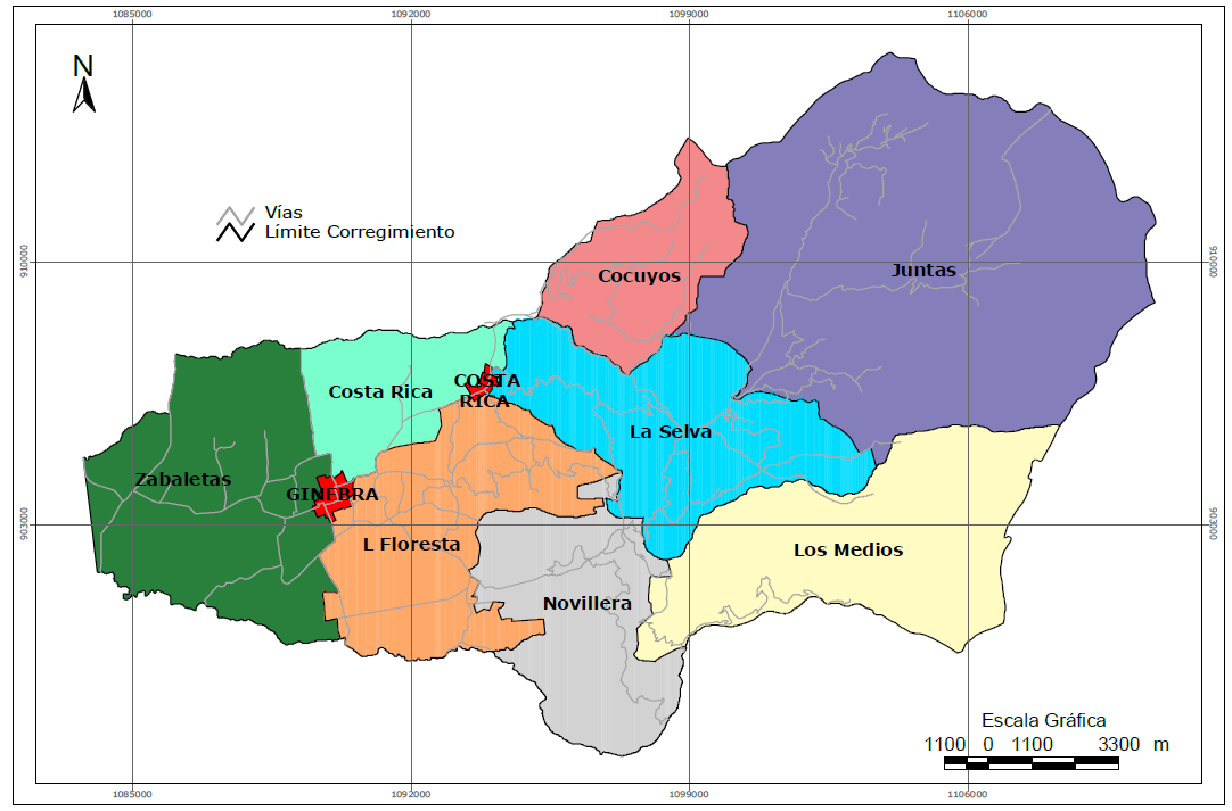
\includegraphics[width=10.7cm]{./imagenes/division_corregimientos}
\caption{División por corregimientos, municipio de Ginebra.}
\end{center}
\end{figure}

\begin{table}[H]
\begin{center}
\begin{tabular}{@{}cc@{}}
\toprule
\textbf{CORREGIMIENTOS} & \textbf{VEREDAS}                                                                                         \\ \midrule
\textbf{JUNTAS}         & \begin{tabular}[c]{@{}c@{}}La Cecilia, Las Hermosas,\\   Portugal, Betania.\end{tabular}                 \\ \midrule 
\textbf{COCUYOS}        & \begin{tabular}[c]{@{}c@{}}Campo Alegre, Moravia, Canaima,\\   Lulos, La cascada, Regaderos\end{tabular} \\ \midrule
\textbf{LA SELVA}       & \begin{tabular}[c]{@{}c@{}}El jardín, El silencio, Cominal,\\   Flautas\end{tabular}                     \\ \midrule
\textbf{COSTA RICA}     & Bello Horizonte, Sauces                                                                                  \\ \midrule
\textbf{LA FLORESTA}    & \begin{tabular}[c]{@{}c@{}}Barranco Bajo, Patio Bonito, Villa\\   Vanegas, Valledupar\end{tabular}       \\ \midrule
\textbf{LA NOVILLERA}   & Barraco Alto, Valledupar                                                                                 \\ \midrule
\textbf{LOS MEDIOS}     & Los Medios                                                                                               \\ \midrule
\textbf{SABALETAS}      & \begin{tabular}[c]{@{}c@{}}El Guabito,  \\ Mosoco\end{tabular}                                           \\ \bottomrule
\end{tabular}
\caption{Listado de Corregimientos y Veredas del Municipio de Ginebra.}
\end{center}
\end{table}

\textit{El Municipio de Ginebra, según proyecciones realizadas por el DANE con base en censo 2005 corregido, tiene en 2008 una población de 18.762 habitantes, ubicando en la cabecera municipal 7.915 (42\% urbana) y 10.893 (58\%) en el área rural."}\cite{4}.

\subsubsection{Gestión del Turismo en Ginebra}
El municipio de Ginebra es reconocido a nivel nacional por el festival de música andina más reconocido del país, el Mono Núñez, en el cual se congregan en promedio 50.000 personas por día. El festival Mono Núñez es el atractivo turístico más reconocido del municipio, pero no el único, también se le reconoce por gastronomía típica vallecaucana lo cual genera que personas de municipios aledaños, sobre todo de la ciudad de Cali\cite{3}. Al ser un municipio con un área rural tan grande también los turistas se acercan para realizar ecoturismo y agroturismo\cite{3}\cite{18} la alcaldía de Ginebra clasifica el turismo del municipio de la siguiente forma:
\vspace{5mm}\newline
\textbf{"Turismo Urbano:} \textit{Es el que se realiza con fines culturales, educativos y recreativos, que da lugar a la conservación y divulgación del patrimonio histórico y cultural, a la creación de espacios públicos de esparcimiento comunitario, y al disfrute de eventos y fiestas culturales, populares y tradicionales. Hacen parte de estas el Festival del Mono Núñez, Las fiestas del Retorno, de la Mora, el Maracuyá entre otras.}
\vspace{5mm}\newline
\textbf{Turismo Gastronómico:} \textit{Es aquel relacionado con la conservación y transmisión de los valores culturales a partir de la tradición regional de la comida. Se desarrolla en los restaurantes y corredores suburbanos Crucero-Ginebra, Crucero la Medina, puente sobre el río Sabaletas; Ginebra-Costa Rica.}
\vspace{5mm}\newline
\textbf{Ecoturismo:} \textit{Aquella forma de turismo especializado y dirigido, que se desarrolla en áreas con un atractivo natural especial que se enmarca dentro de los parámetros del desarrollo humano sostenible, en busca de la recreación, esparcimiento y la educación del visitante a través de la observación, el estudio de los valores naturales y los aspectos culturales relacionados con ellos. Franjas del río Guabas desde Flautas hasta las Hermosas; franjas forestales de los Medios y Novillera; Franjas de la vereda La Selva.}
\vspace{5mm}\newline
\textbf{Agroturismo:} \textit{El agroturismo es un tipo de turismo especializado en el cual el turista se involucra con el campesino en las labores agrícolas. Franja de la vereda La Floresta, corredor suburbano Ginebra- Santa Helena."\cite{18}.}

\section{Antecedentes}
La creciente importancia de las nuevas tecnologías y el marketing digital hace necesario el estudio del impacto que tendrán estos aspectos en el negocio empresarial, más concretamente en aquellos sectores que son más importantes, en este trabajo nos enfocaremos en el área del turismo.
La tipología de aplicaciones relacionadas de forma más o menos directa con la actividad turística es de lo más variado, hasta el punto de que alojamientos turísticos, empresas de creación de productos turístico-culturales, espacios de presentación del patrimonio y destinos (ciudades, regiones, países) han comprendido el cambio experimentado y generan cada vez más recursos en forma de apps para el consumo turístico. 
Desde el punto de vista de los destinos turísticos, cada vez son más los que ofrecen desde sus sitios web un listado de las aplicaciones más útiles para el turista, a modo de compendio, en el ánimo de facilitarle a aquel la organización del viaje y de poner a su disposición los recursos que le pueden ser de más utilidad.
Para el destino, no solo le garantiza un retorno de inversión, sino que se conforma como herramienta clave para promocionar bienes de interés cultura, o para conocer el perfil del visitante, muy útil para alcanzar la excelencia de los destinos turísticos culturales. \cite{19}–\cite{21}

\subsection{DataEco\cite{22}}
DataEco (Dataset Ecoturístico del Centro del Valle) es un dataset con información ecoturística de los municipios de Tuluá y Riofrío pertenecientes a la Subregión Centro del Departamento del Valle del Cauca, con el cual se facilitan las tareas de búsqueda, clasificación y enriquecimiento semántico de la información ecoturística de esta región.
La información presente se centra en cuatro rutas ecoturísticas del municipio de Tuluá denominadas ruta del maíz, ruta vuelta a oriente, ruta jardín botánico y ruta anillo agrícola. Por cada ruta se puede encontrar información sobre restaurantes, alojamientos, lugares, eventos, fauna, flora, entre otros.
Del mismo modo, se puede encontrar información ecoturística del municipio de Riofrio, caracterizado por ser uno de los líderes del sector turismo de la región

\subsection{Google Maps\cite{23}}
Google Maps es un servidor de aplicaciones de mapas en la web, ofrece imágenes de mapas desplazables, así como fotografías por satélites del mundo e incluso la ruta entre diferentes ubicaciones o imágenes a pie de calle con Google Street View.
Google Maps ofrece una serie de beneficios para los negocios, dentro de estos se encuentra: 
\begin{itemize}
    \item Vistas de mapas de tipo nominal, satelital y terreno.
    \item Destinos múltiples para ver las paradas en transporte público.
    \item Simplicidad que permite ubicar rápidamente un negocio.
    \item Tipo de Viaje para elegir en qué medio de transporte viajar y obtener el camino a seguir para llegar al lugar deseado.
    \item Adaptable ambiente móvil.
    \item Opción zoom que permite ubicarse exactamente donde se encuentra el negocio.
    \item Descripción del negocio que muestra un pequeño resumen del negocio: nombre del negocio, teléfono, logo, sitio web, etc., haciendo más relevante la credibilidad y confianza del negocio.
\end{itemize}

\subsection{Foursquare\cite{24}, \cite{25}}
Foursquare es un servicio basado en la localización web aplicada a las redes sociales que ayuda a descubrir nuevos lugares con las recomendaciones que hace la comunidad.
La idea principal de esta red es marcar (check-in) lugares específicos donde uno se encuentre e ir ganando puntos por "descubrir" nuevos lugares.
Las recompensas que se obtienen son las "badges", una especie de medallas, y las "Alcaldías" que son ganadas por las personas que más hacen check-in en un cierto lugar en los últimos 60 días.
El servicio es alimentado por los usuarios, quienes construyen la base de datos de los sitios y la comparten con el resto de la comunidad. Este servicio presenta una limitación y es que los usuarios no pueden valorar y opinar acerca de los negocios que aparecen.
%%%%%%%%%%%%%%%%%%%%%%%%%%%%%%%%%%%%%%%%%%%%%%%%%%%%%%%%%%%%%%%%%%%%%%%%%%%%%%%%%%%%%%%%%%
%%%%%%%%%%%%%%%%%%%%%%%%%%%%%%						FIN MARCO DE REFERENCIA
%%%%%%%%%%%%%%%%%%%%%%%%%%%%%%%%%%%%%%%%%%%%%%%%%%%%%%%%%%%%%%%%%%%%%%%%%%%%%%%%%%%%%%%%%%

%%%%%%%%%%%%%%%%%%%%%%%%%%%%%%%%%%%%%%%%%%%%%%%%%%%%%%%%%%%%%%%%%%%%%%%%%%%%%%%%%%%%%%%%%%%%%%%%%%
%%%%%%%%%%%%%%%%%%%%%%%%%%%%%%%%%%%%%%%%%%%%%%%%%%%%%%%%%%%%%%%%%%%%%%%%%%%%%%%%%%%%%%%%%%%%%%%%%%
%%%%%%%%%%%%%%%%%%%%%%%%%%%%%%%%%%%%%%%%%%%%%%%%%%%%%%%%%%%%%%%%%%%%%%%%%%%%%%%%%%%%%%%%%%%%%%%%%%
%%%%%%%%%%%%%%%%%%%%%%%%%%%%%%%%%%%%%%%%%%%%%%%%%%%%%%%%%%%%%%%%%%%%%%%%%%%%%%%%%%%%%%%%%%%%%%%%%%

%%%%%%%%%%%%%%%%%%%%%%%%%%%%%%%%%%%%%%%%%%%%%%%%%%%%%%%%%%%%%%%%%%%%%%%%%%%%%%%%%%%%%%%%%%
%%%%%%%%%%%%%%%%%%%%%%%%%%%%%%						DESARROLLO DEL PROYECTO
%%%%%%%%%%%%%%%%%%%%%%%%%%%%%%%%%%%%%%%%%%%%%%%%%%%%%%%%%%%%%%%%%%%%%%%%%%%%%%%%%%%%%%%%%%
\chapter{Desarrollo del Proyecto}\label{cap.desarrollo_del_proyecto}
Para el desarrollo de este proyecto, se utilizó la metodología Mobile-D.
Mobile-D es considerada nueva para el desarrollo de aplicaciones móviles, propuesta por Pekka Abrahamsson y su equipo del VTT (Valtion Teknillinen Tutkimuskeskus) en Finlandia que lideran una corriente muy importante de desarrollo ágil, muy centrado en las plataformas móviles.
La metodología Mobile-D consta de 5 fases: exploración, iniciación, producción, estabilización y prueba del sistema. 
\begin{itemize}
    \item Exploración: Esta fase se enfoca en planear y establecer el proyecto. 
    \item Inicialización: Preparar y verificar todas las cuestiones relacionadas con el proyecto. 
    \item Producción: Se encarga de hacer la implementación requerida del proyecto. 
    \item Estabilización: Se finaliza la implementación del producto y se realizan mejoras. 
    \item Prueba y arreglos del sistema: Se hacen pruebas y solucionan errores.
\end{itemize}

\begin{figure}[H]
\begin{center}
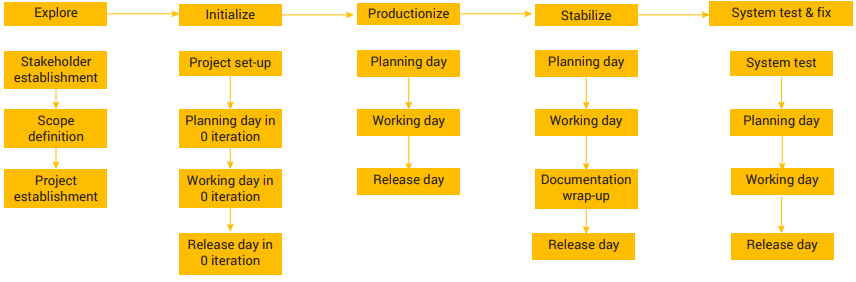
\includegraphics[width=16cm]{./imagenes/ciclo_desarrollo}
\caption{Ciclo de desarrollo Mobile-D.}
\end{center}
\end{figure}

En la fase de \textbf{exploración},  se levantan requerimientos y se realiza un diseño general del sistema mediante el diseño de la arquitectura del sistema de alto nivel y los casos de uso.
\\
En la fase de \textbf{inicialización}, de acuerdo a los requerimientos levantados, se realizan las historias de usuario y los diagramas de colaboración y secuencia en base a los casos de uso realizados. De igual manera, se realiza el diagrama de entidad-relación de la base de datos, y el diagrama de clases de la aplicación móvil.
\\
En la fase de \textbf{producción}, se comienza a desarrollar los módulos que se requieren para cumplir con los requerimientos levantados. En el backend, se crean las APIs de acuerdo al modelo de la base de datos y sus peticiones HTTP, según su requerimiento (GET, POST, PUT, DELETE, etc). En el frontend, se realiza la aplicación móvil de acuerdo al diseño planteado.
\\
En la fase de \textbf{estabilización}, se integran los modulos desarrollados tanto del Backend como del Frontend, utilizando el sistema de version de controles github mediante peticiones pull request.
\\
En la fase de \textbf{pruebas} se realizan pruebas de aceptación de acuerdo a las historias de usuario, pruebas unitarios al backend y a la aplicación, y pruebas de usabilidad en el frontend.
\\
La evidencia del trabajo realizado se puede observar en las siguientes figuras:
\begin{figure}[H]
\begin{center}
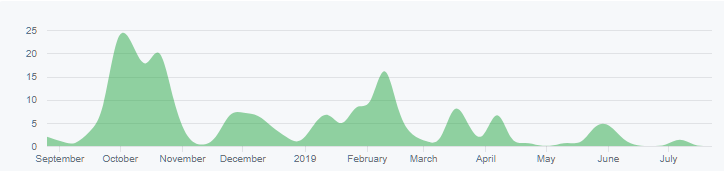
\includegraphics[width=13cm]{./imagenes/commitsApp}
\caption{Commits realizados en GitHub para la Aplicación Móvil.}
\end{center}
\end{figure}

\begin{figure}[H]
\begin{center}
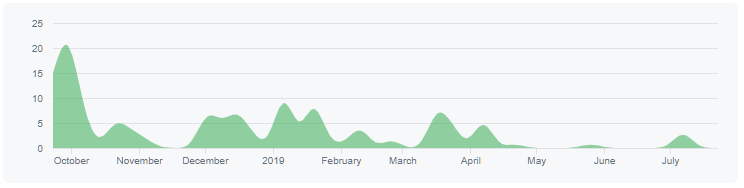
\includegraphics[width=13cm]{./imagenes/commitsBackend}
\caption{Commits realizados en GitHub para el Backend.}
\end{center}
\end{figure}

\section{Arquitectura del Sistema Implementado}
La siguiente figura describe el esquema o funcionamiento de la aplicación y evidencia cada uno de los componentes que se relacionan entre sí, la arquitectura utilizada fue de tipo cliente – servidor. Para la generación de recomendación automática se hizo la utilización de otro lenguaje de programación diferente a JAVA, en este caso Python fue el seleccionado, usando el framework Django y Django-Rest-Framework.
\begin{figure}[H]
\begin{center}
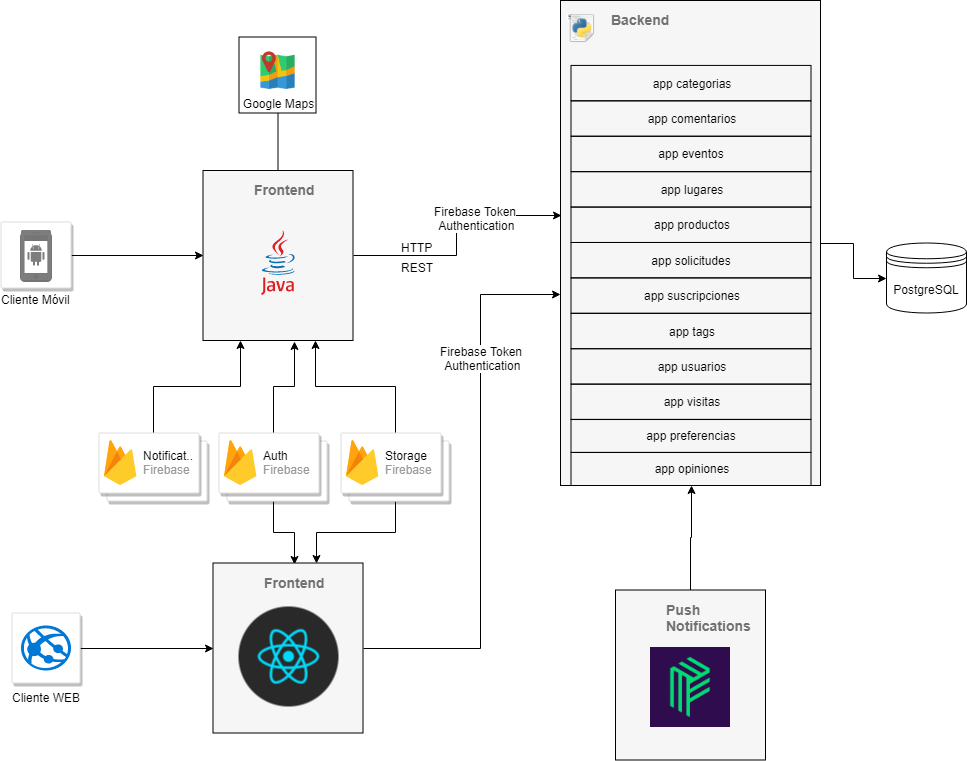
\includegraphics[width=13cm]{./imagenes/arquitectura}
\caption{Arquitectura del Sistema.}
\end{center}
\end{figure}


\section{Diseño}
\subsection{Historias de Usuarios}
\begin{table}[H]
\centering
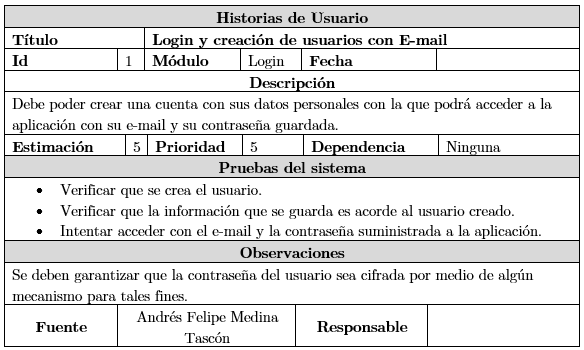
\includegraphics[width=9cm]{./imagenes/HU/HU1}
\caption{HU1: Login y creación de usuarios con E-mail.}
\end{table}

\begin{table}[H]
\centering
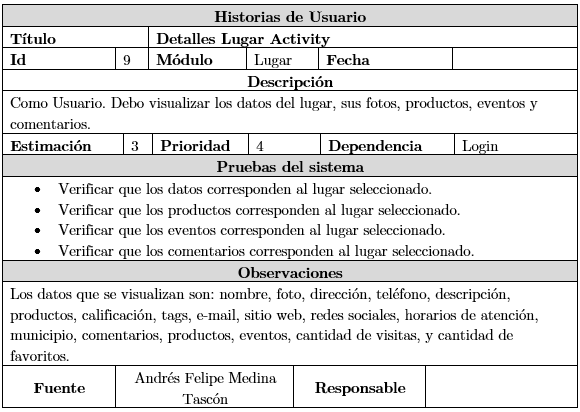
\includegraphics[width=9cm]{./imagenes/HU/HU9}
\caption{HU9 Detalles Lugar Activity.}
\end{table}

\begin{table}[H]
\centering
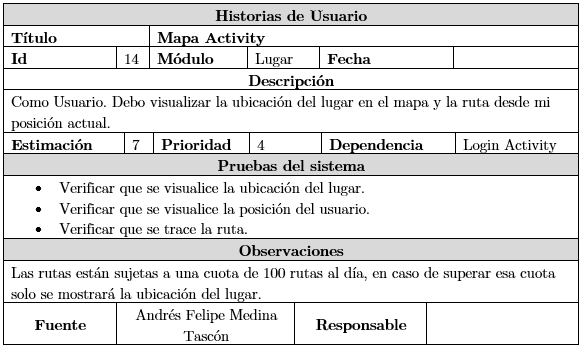
\includegraphics[width=9cm]{./imagenes/HU/HU14}
\caption{HU14 Mapa Activity.}
\end{table}

Las demás Historias de Usuario realizadas las puede detallar en el documento Anexo, Apéndice A.

\subsection{Diagrama Entidad - Relación}
\begin{figure}[H]
\begin{center}
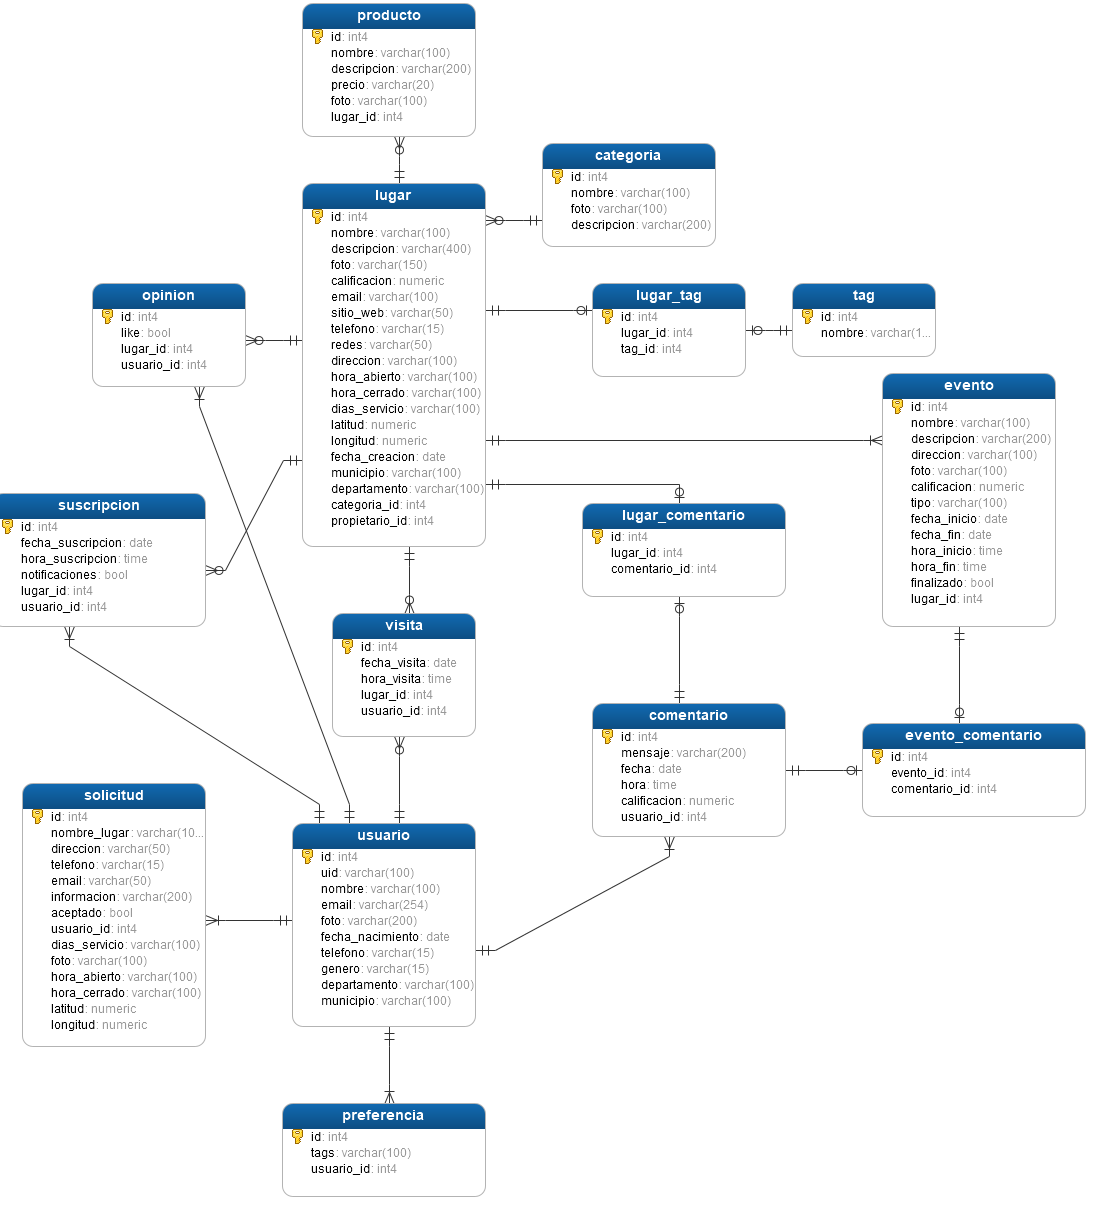
\includegraphics[width=16cm]{./imagenes/Diagrama_entidad_relacion}
\caption{Diagrama Entidad - Relación.}
\end{center}
\end{figure}

\subsection{Diagrama de Clases}
\begin{figure}[H]
\begin{center}
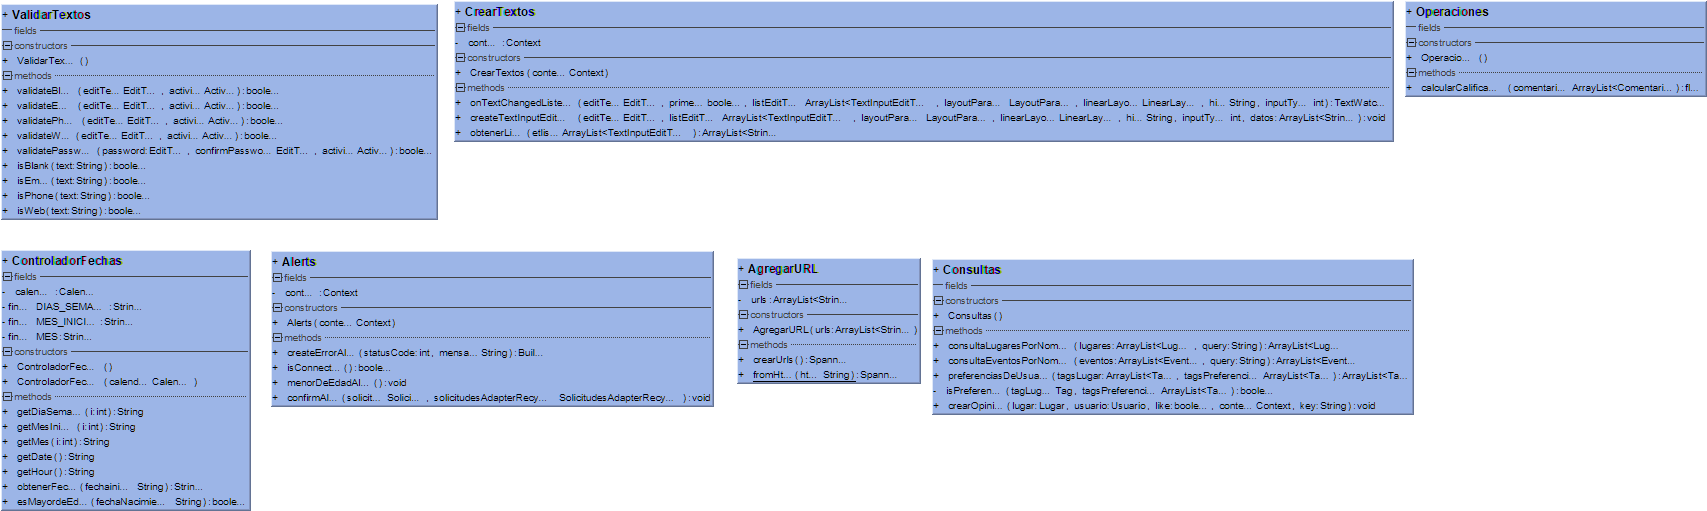
\includegraphics[width=16cm]{./imagenes/diagrama_clases}
\caption{Diagrama de clases.}
\end{center}
\end{figure}

\subsection{Diagrama de Ventanas}
\begin{figure}[H]
\begin{center}
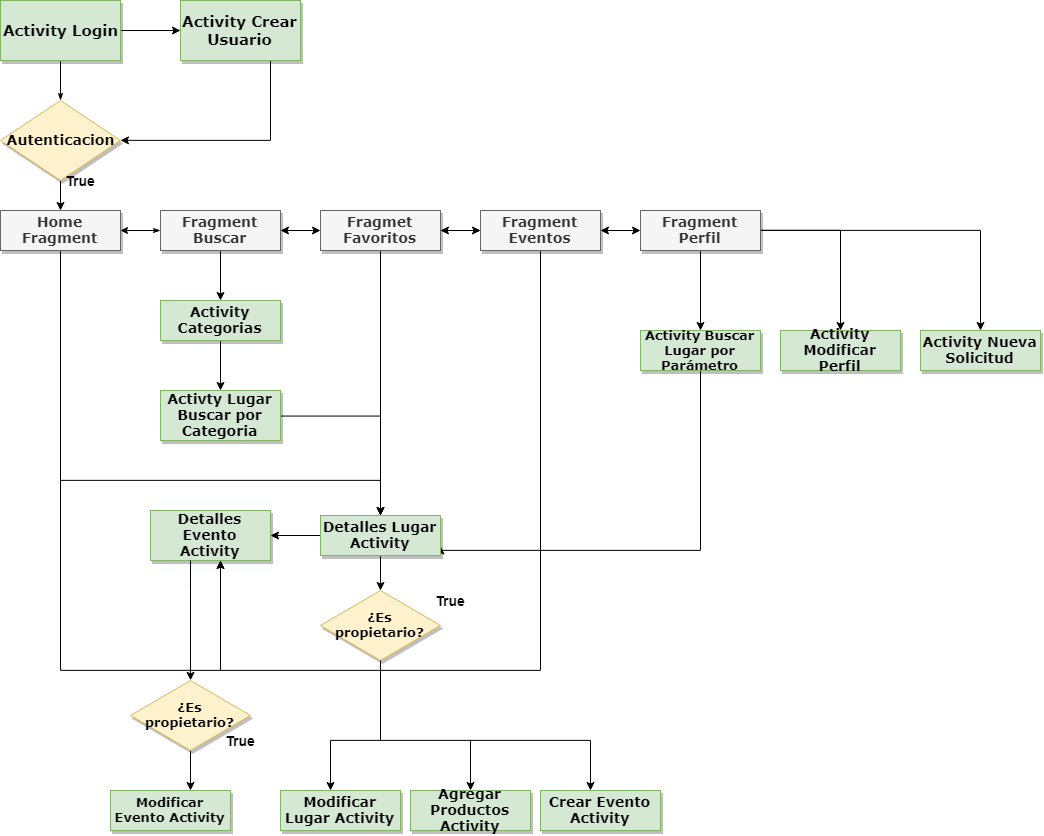
\includegraphics[width=13cm]{./imagenes/diagrama_ventanas}
\caption{Diagrama de Ventanas.}
\end{center}
\end{figure}

\subsection{Diagramas de Casos de Uso}
Un caso de uso representa un proceso común e importante. Los casos de uso constituyen una técnica para la captura de requisitos potenciales de un nuevo sistema o una actualización de software. Un diagrama de caso de uso muestra las distintas operaciones que se esperan de una aplicación o sistema y como se relaciona con su entorno (usuarios u otras aplicaciones).
\vspace{5mm}\newline
\textbf{Administrador:} En el diagrama de casos de uso de la figura están representados los casos de uso en los cuales participa el administrador del sistema de gestión de la aplicación.
\begin{figure}[H]
\begin{center}
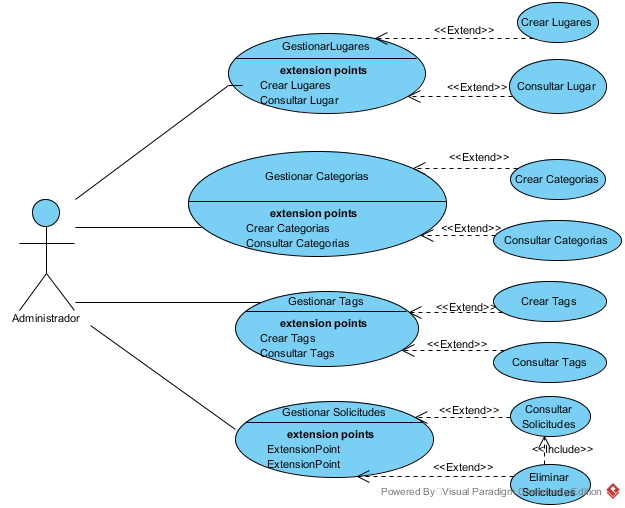
\includegraphics[width=10cm]{./imagenes/CU/cu_administrador}
\caption{Caso de Uso Administrador.}
\end{center}
\end{figure}

\textbf{Usuario:} En el diagrama de casos de uso de la figura están representados los casos de uso en los cuales participa el usuario del aplicativo móvil.
\begin{figure}[H]
\begin{center}
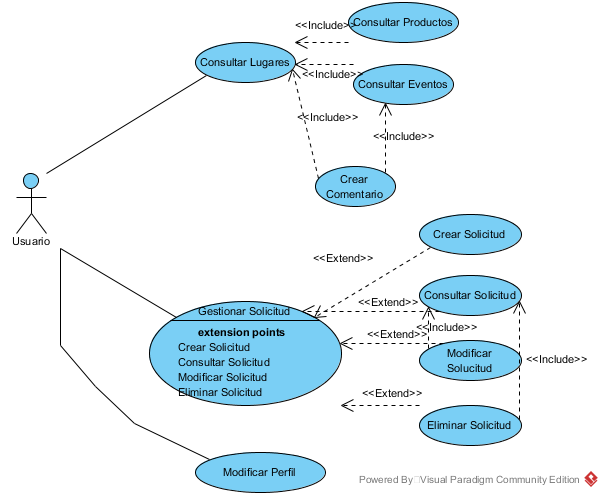
\includegraphics[width=10cm]{./imagenes/CU/cu_usuario}
\caption{Caso de Uso Usuario.}
\end{center}
\end{figure}

\textbf{Comerciante:} En el diagrama de casos de uso de la figura están representados los casos de uso en los cuales participa el usuario comerciante del aplicativo móvil.
\begin{figure}[H]
\begin{center}
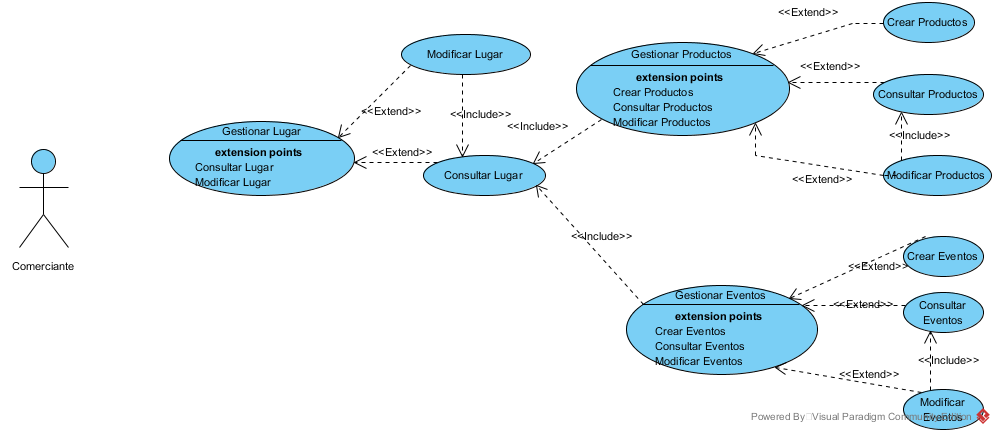
\includegraphics[width=13cm]{./imagenes/CU/cu_comerciante}
\caption{Caso de Uso Comerciante.}
\end{center}
\end{figure}

\subsection{Plantillas Especificación Casos de Uso}
\begin{table}[H]
\centering
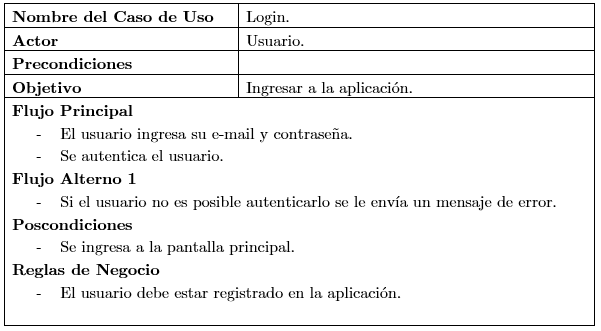
\includegraphics[width=13cm]{./imagenes/PCU/login}
\caption{Plantilla Especificación Caso de Uso Login.}
\end{table}

\begin{table}[H]
\centering
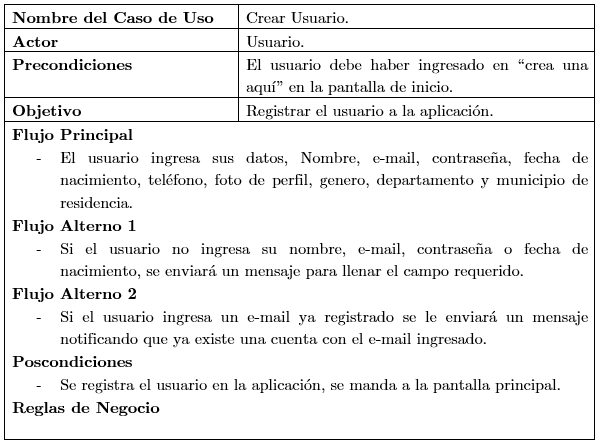
\includegraphics[width=13cm]{./imagenes/PCU/crear_usuario}
\caption{Plantilla Especificación Caso de Uso Crear Usuario.}
\end{table}

\begin{table}[H]
\centering
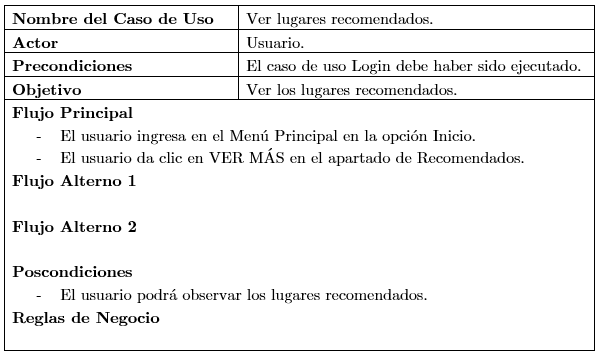
\includegraphics[width=13cm]{./imagenes/PCU/ver_lugares_recomendados}
\caption{Plantilla Especificación Caso de Uso Ver lugares recomendados.}
\end{table}

Las demás Plantillas de Especificación de Casos de Uso realizadas las puede detallar en el documento Anexo, Apéndice B.

\subsection{Diagramas de Secuencia y Colaboración}
Los diagramas de secuencia permiten visualizar la interacción de los diferentes objetos y actores a través del tiempo. Los diagramas de colaboración contienen la misma información que los diagramas de secuencia, solo que se centran en las responsabilidades de cada objeto, en lugar del tiempo. En las siguientes figuras se encontraran algunos de los diagramas de secuencia y colaboración de los casos de uso descritos anteriormente.

\begin{figure}[H]
\begin{center}
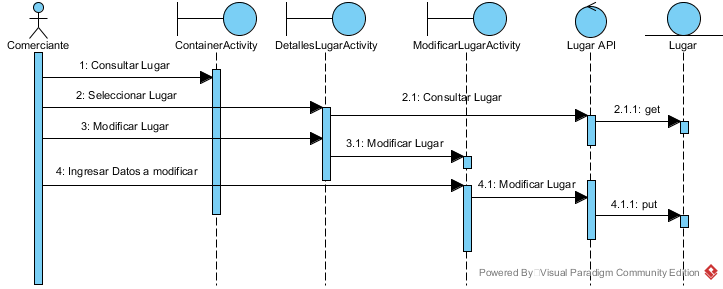
\includegraphics[width=10cm]{./imagenes/DS/DS_gestionar_lugar}
\caption{Diagrama de Secuencia Gestionar Lugar.}
\end{center}
\end{figure}

\begin{figure}[H]
\begin{center}
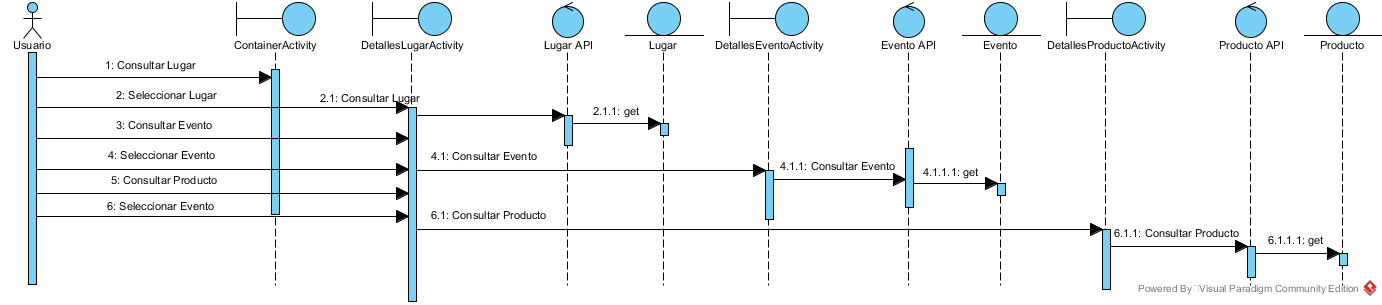
\includegraphics[width=14cm]{./imagenes/DS/DS_consultar_lugares}
\caption{Diagrama de Secuencia Consultar Lugares.}
\end{center}
\end{figure}



\begin{figure}[H]
\begin{center}
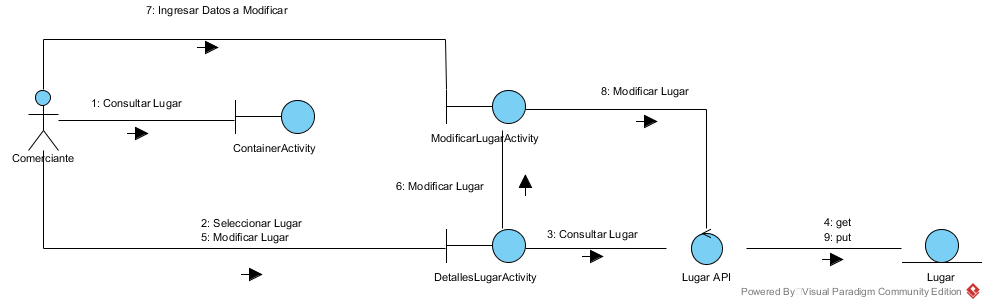
\includegraphics[width=14cm]{./imagenes/DC/DC_gestionar_lugar}
\caption{Diagrama de Colaboración Gestionar Lugar.}
\end{center}
\end{figure}

\begin{figure}[H]
\begin{center}
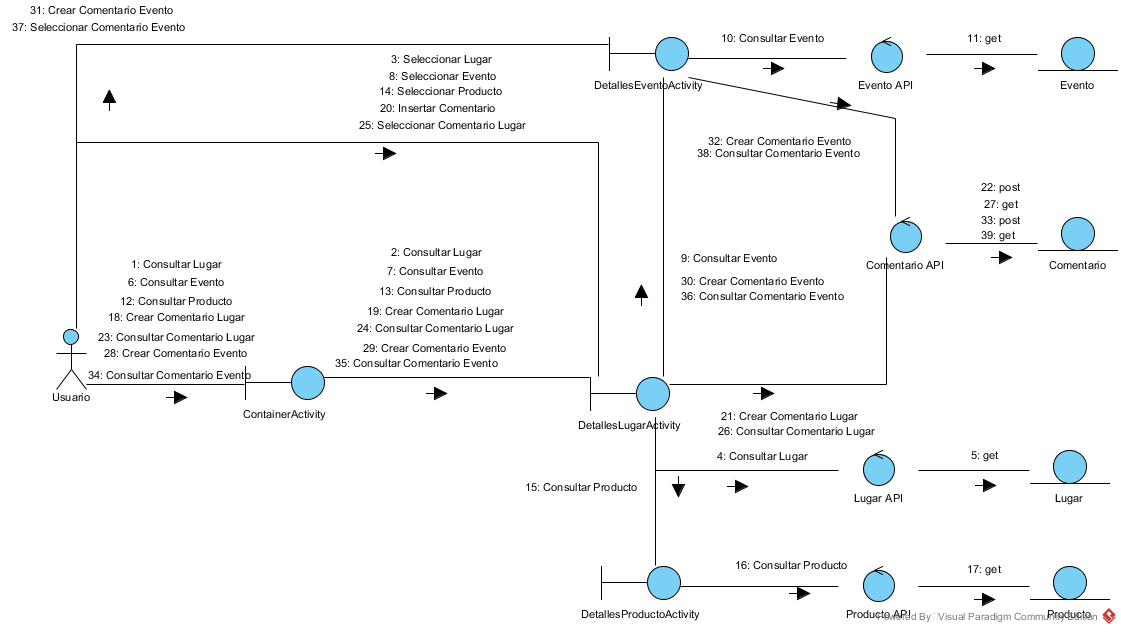
\includegraphics[width=14cm]{./imagenes/DC/DC_consultar_lugar}
\caption{Diagrama de Colaboración Consultar Lugares.}
\end{center}
\end{figure}

Los demás Diagramas de Secuencia y Colaboración realizados las puede detallar en el documento Anexo, Apéndice C.

\section{Descripción General del Sistema}
\subsection{Interfaz Gráfica de Usuario}
La interfaz gráfica de usuario pone a disposición los métodos y funcionalidades desarrolladas para la sistematización de la información referente a los lugares. La siguiente figura evidencia la pantalla principal de la aplicación para el usuario.

\begin{figure}[H]
\begin{center}
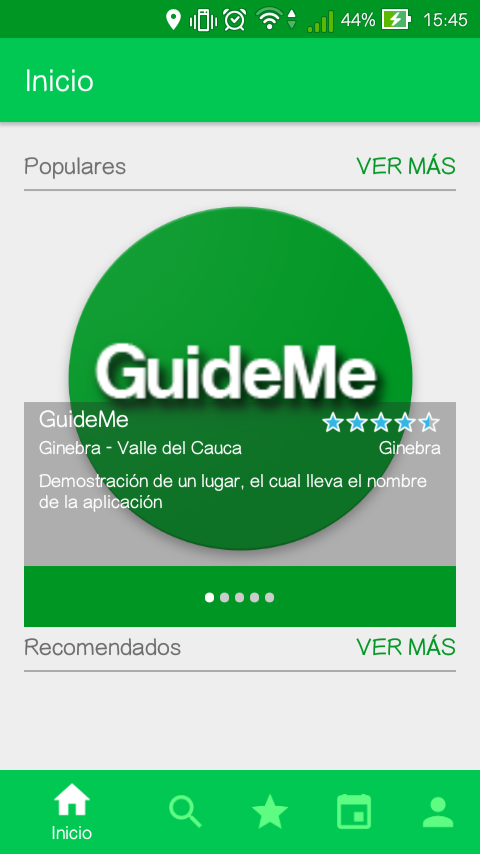
\includegraphics[width=4cm]{./imagenes/gui}
\caption{Aspecto Inicial de la Aplicación para un usuario logeado.}
\end{center}
\end{figure}

\subsection{Administrador}
Para la administración de la aplicación móvil, se implementó un \textbf{servicio web} el cual permite al administrador, la creación de los sitios que aparecerán dentro del app, las diferentes categorías y los tags, como también revisar las solicitudes recibidas para registrar nuevos lugares por parte de los usuarios.
\vspace{5mm}\newline
Para el desarrollo del servicio web, se hizo uso de ReactJS, una biblioteca Javascript de código abierto, la cual fue diseñada para crear interfaces de usuario con el objetivo de facilitar el desarrollo de aplicaciones en una sola página.

\subsubsection{Autenticación}
En la siguiente pantalla, el administrador ingresa su usuario y contraseña en el servicio web para identificarse como tal y poder realizar alguna de las funciones previamente mencionadas.

\begin{figure}[H]
\begin{center}
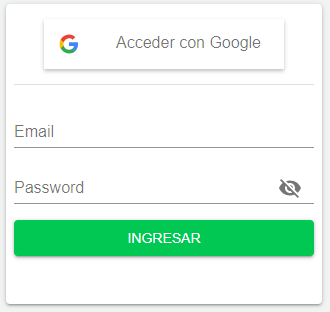
\includegraphics[width=4cm]{./imagenes/admin/login}
\caption{Login Web Service.}
\end{center}
\end{figure}

Una vez el administrador ha ingresado al sistema, tendrá en pantalla las opciones permitidas para él.

\begin{figure}[H]
\begin{center}
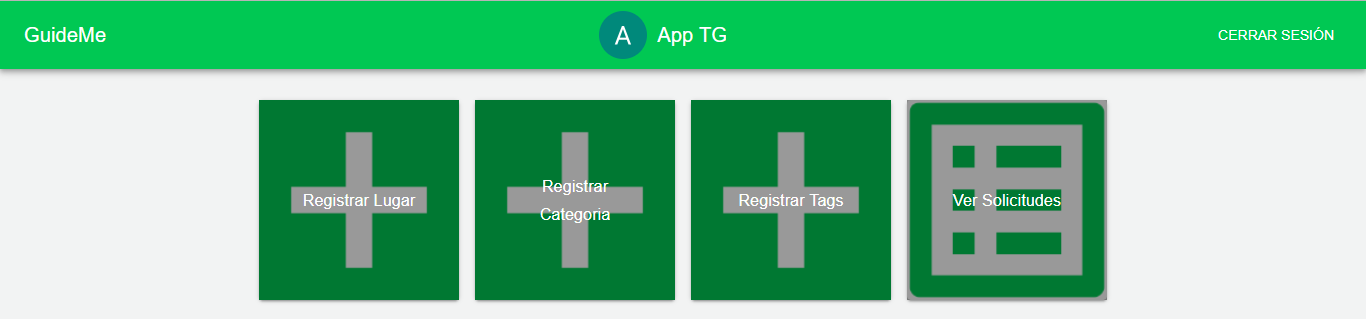
\includegraphics[width=13cm]{./imagenes/admin/p_principal}
\caption{Pantalla Principal Menú Administrador.}
\end{center}
\end{figure}

\subsubsection{Registrar Lugar}
En la siguiente pantalla, el administrador registra los datos asociados a un nuevo lugar. \\
Si el registro se realiza desde la pestaña de solicitudes, el propietario del lugar será la persona que realizo la solicitud, mientras si se realiza desde la pestaña crear lugar, el propietario sera el administrador de manera temporal.

\begin{figure}[H]
\begin{center}
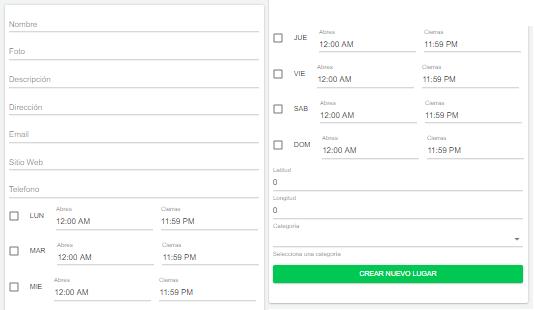
\includegraphics[width=9cm]{./imagenes/admin/crear_lugar}
\caption{Registrar Lugar.}
\end{center}
\end{figure}

\subsubsection{Registrar Categoría}
En la siguiente pantalla, el administrador registra los datos asociados a una nueva categoría.
Las categorías son usadas para poder clasificar los lugares disponibles en la aplicación.
\begin{figure}[H]
\begin{center}
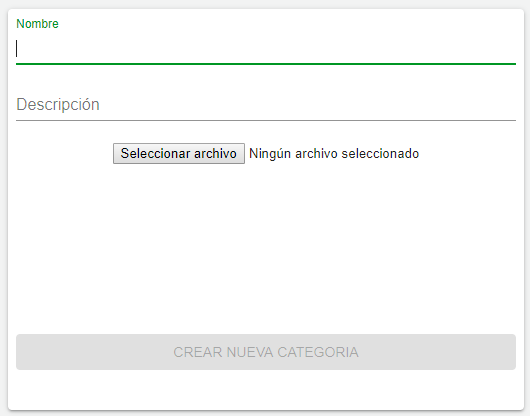
\includegraphics[width=8cm]{./imagenes/admin/r_categoria}
\caption{Registrar Categoría.}
\end{center}
\end{figure}

Las imágenes que se cargan en esta pantalla se almacenan en Firebase, utilizado para la autenticación de los usuarios y almacenamiento de multimedia. Se hace un llamado a la URL de la ubicación de la imagen cuando es solicitada por la aplicación desde el celular del usuario.

\subsubsection{Registrar Tag}
En la siguiente pantalla, el administrador registra tags, los cuales serán claves para identificar a los lugares, y para poder generar recomendaciones a los usuarios.
\begin{figure}[H]
\begin{center}
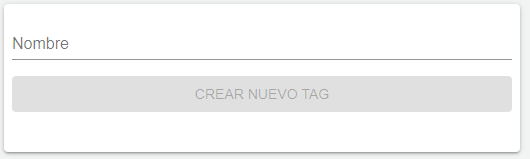
\includegraphics[width=10cm]{./imagenes/admin/r_tags}
\caption{Registrar Tag.}
\end{center}
\end{figure}

\subsubsection{Ver Solicitudes}
En la siguiente pantalla, el administrador revisará las solicitudes recibidas para registrar nuevos lugares en la aplicación. El administrador puede decidir que solicitud aceptar, o rechazar.

\begin{figure}[H]
\begin{center}
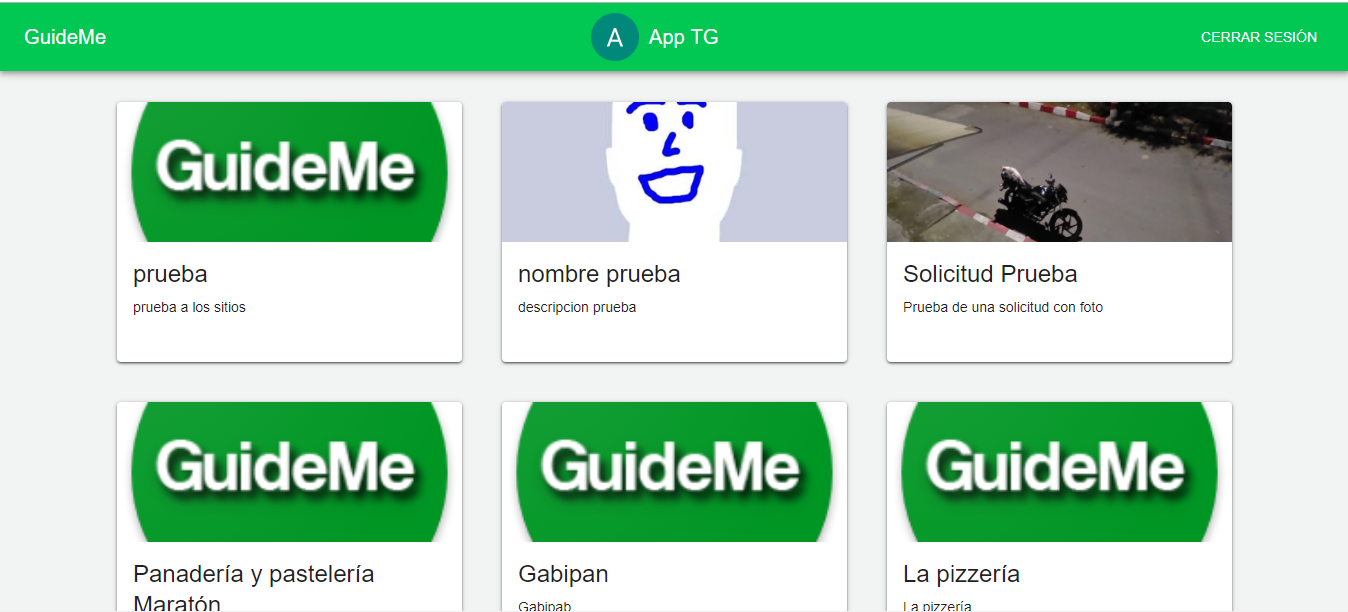
\includegraphics[width=10cm]{./imagenes/admin/solicitudes}
\caption{Solicitudes Recibidas.}
\end{center}
\end{figure}

\subsection{Usuario}
\subsubsection{Pantalla Principal}
La pantalla principal (Figura 3.8) está compuesta por diferentes secciones: \\
Lugares populares: Son los que contengan la puntuación y el numero de comentarios más alto.\\
Lugares recomendados: Son los que coincidan con las preferencias del usuario, dichas preferencias se podrán elegir al momento de crear una cuenta.\\
Lugares nuevos: Son los lugares cuya fecha de registro se encuentra entre la fecha actual, y un parámetro de días establecidos.\\
Por ultimo, en caso de existir eventos disponibles realizados por los lugares a los cuales el usuario sigue, aparecerán también  en pantalla.
\begin{figure}[H]
\begin{center}
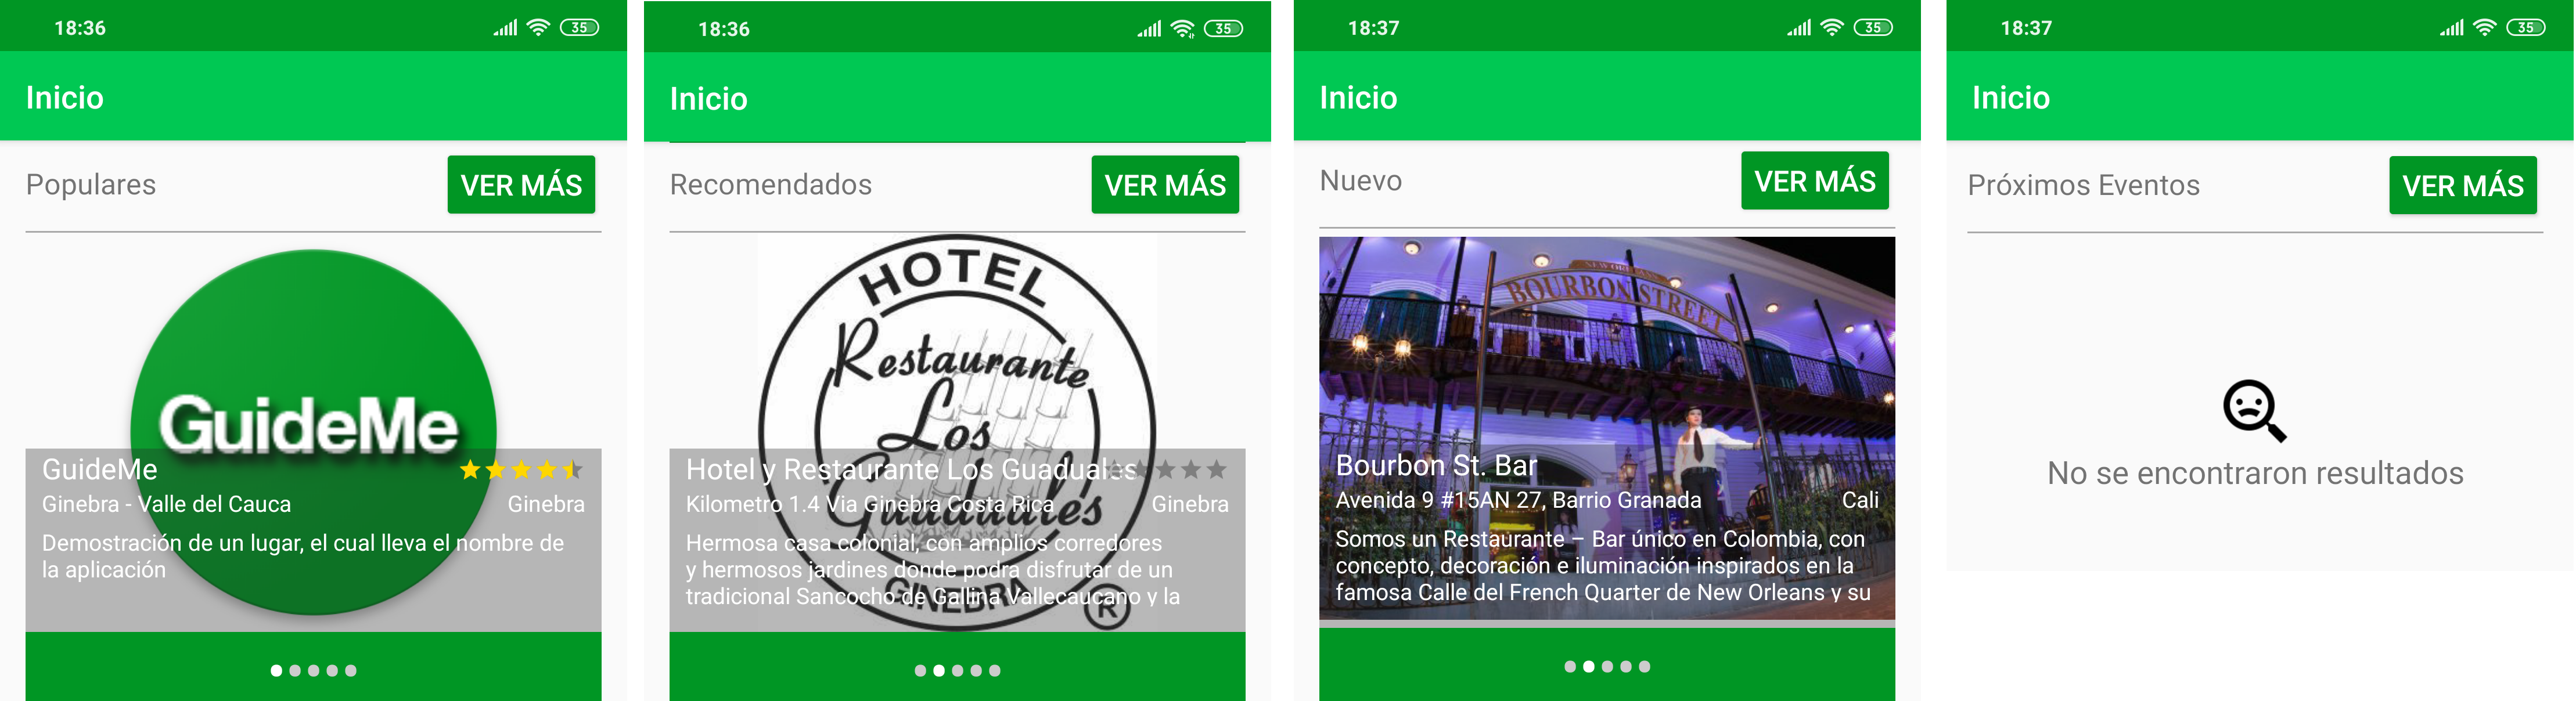
\includegraphics[width=14cm]{./imagenes/1}
\caption{Secciones Pantalla Principal.}
\end{center}
\end{figure}

\subsubsection{Buscar Lugares}
En la sección de búsquedas, es posible filtrar lugares por categorías (Vida Nocturna, Desayuno, Entretenimiento, Restaurante, Comida Rápida, Hospedaje), así como también filtrarlos por parte de su nombre.
\vspace{5mm}\newline
Una vez ejecutada la búsqueda, aparece en pantalla los lugares que coincidan con el criterio establecido, y un botón para poder ver su ubicación en el mapa.
\begin{figure}[H]
\begin{center}
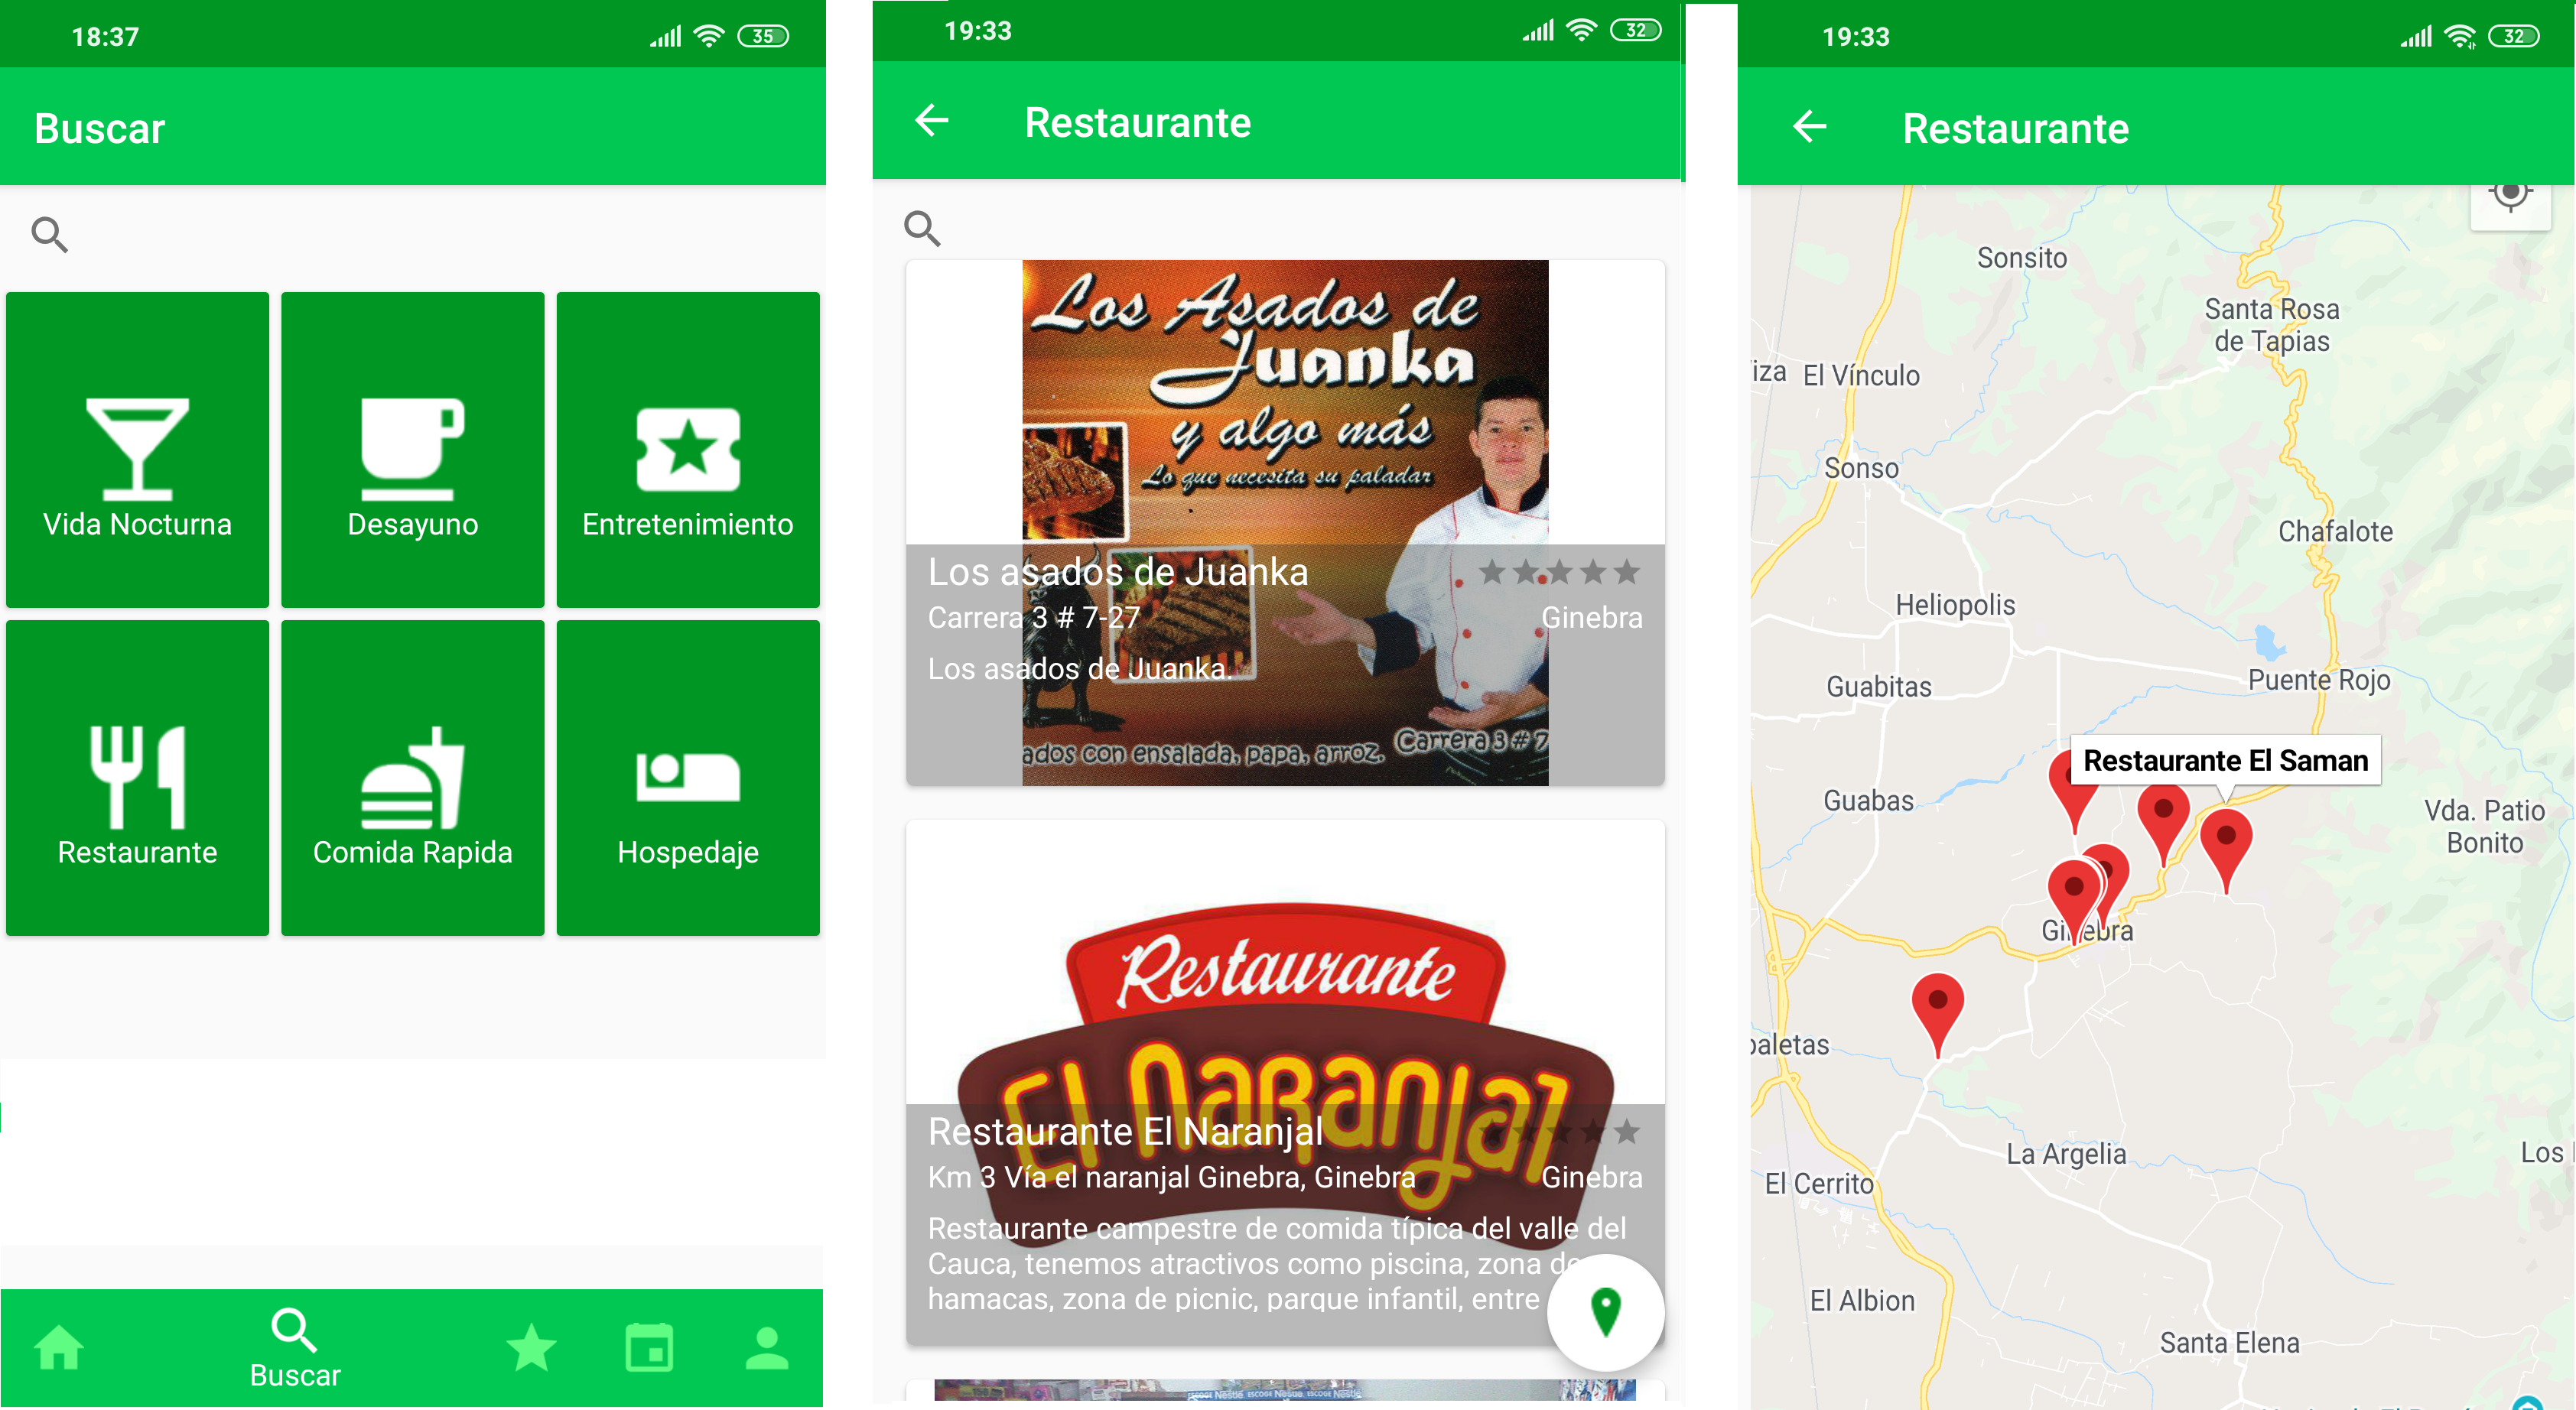
\includegraphics[width=10cm]{./imagenes/2}
\caption{Pantalla búsquedas, resultados obtenidos filtrados por categoría y ubicación en el mapa.}
\end{center}
\end{figure}

\subsubsection{Lugares favoritos}
En la sección de lugares favoritos, aparecen los lugares a los cuales el usuario ha decidido seguir.\\
Es posible realizar la búsqueda de los lugares favoritos como criterio de búsqueda parte de su nombre.
\begin{figure}[H]
\begin{center}
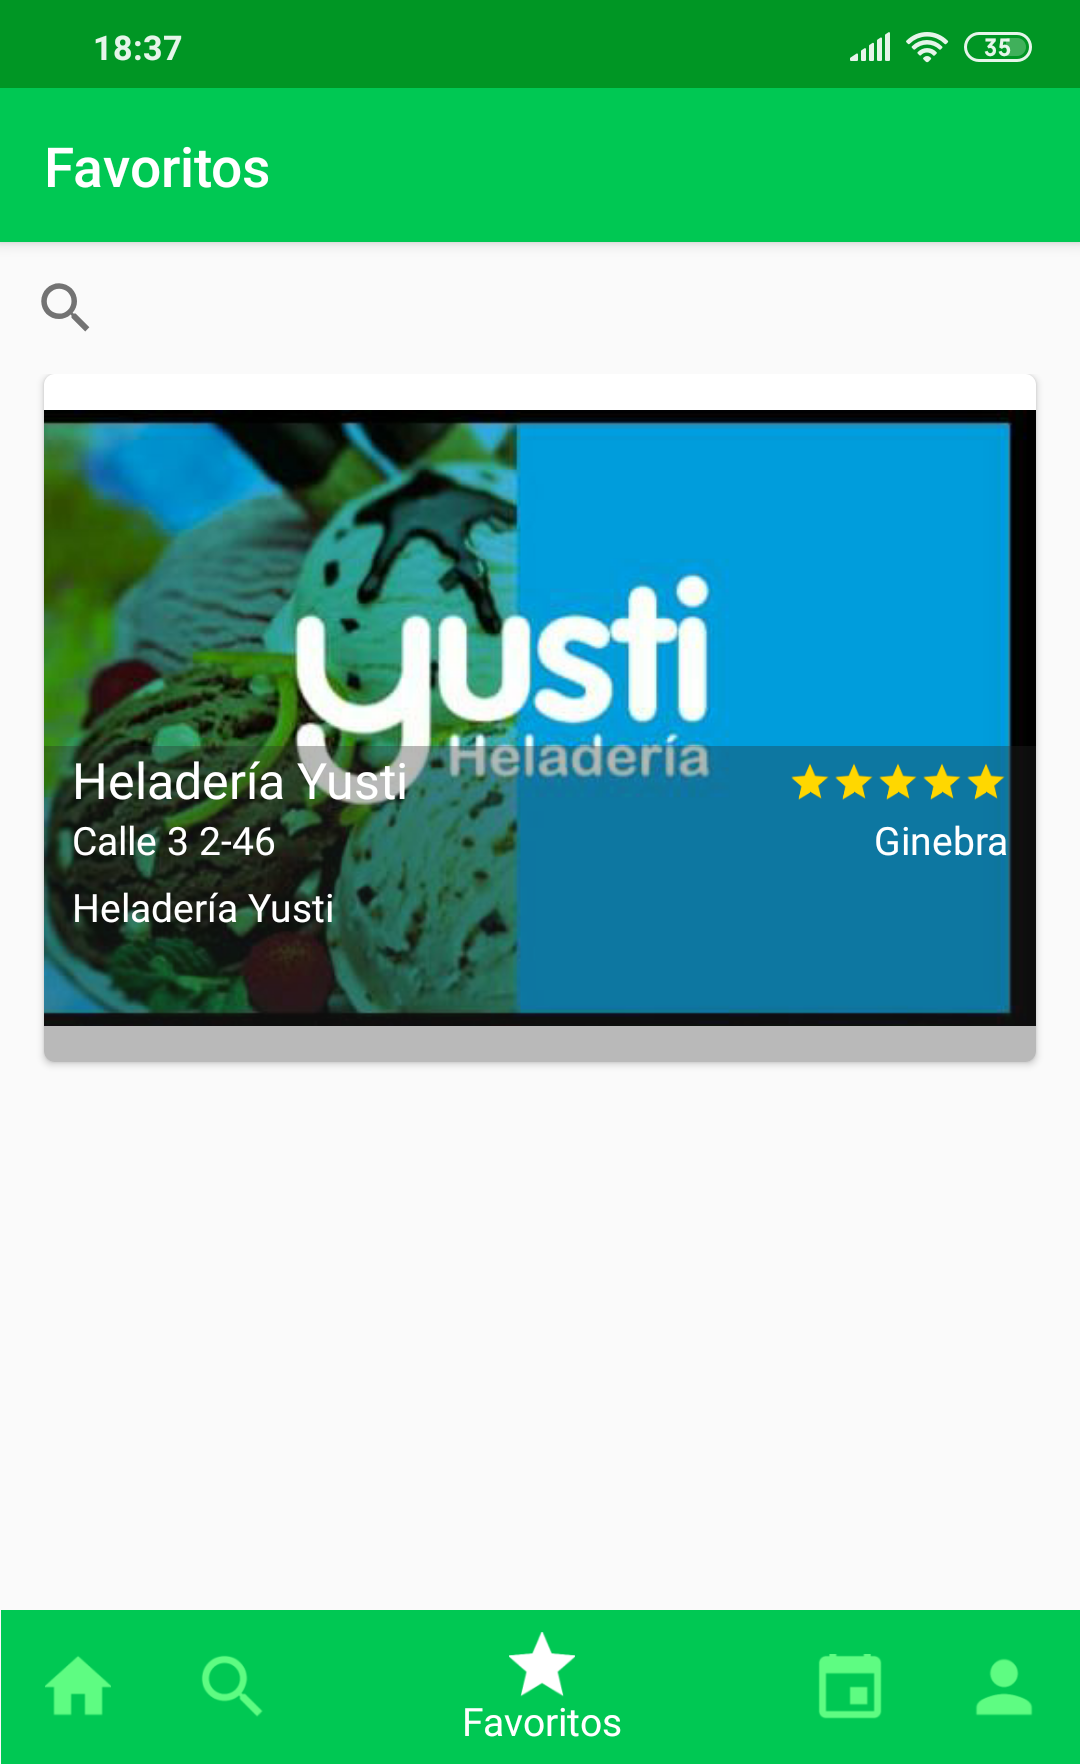
\includegraphics[width=4cm]{./imagenes/3}
\caption{Lugares Favoritos.}
\end{center}
\end{figure}

\subsubsection{Detalles de un lugar}
Desde la pantalla principal, la sección de búsquedas o la sección lugares favoritos, es posible visualizar la información referente a un lugar deseado al entrar a este.
\vspace{5mm}\newline
La información que el usuario verá acerca de un lugar será nombre, fotos, dirección, teléfono, descripción, productos, calificación, tags, e-mail, sitio web, redes sociales, horarios de atención, municipio, comentarios, productos, eventos, cantidad de visitas, y cantidad de favoritos.\\
También es posible visualizar en un mapa su ubicación y la ruta para llegar a este.
\begin{figure}[H]
\begin{center}
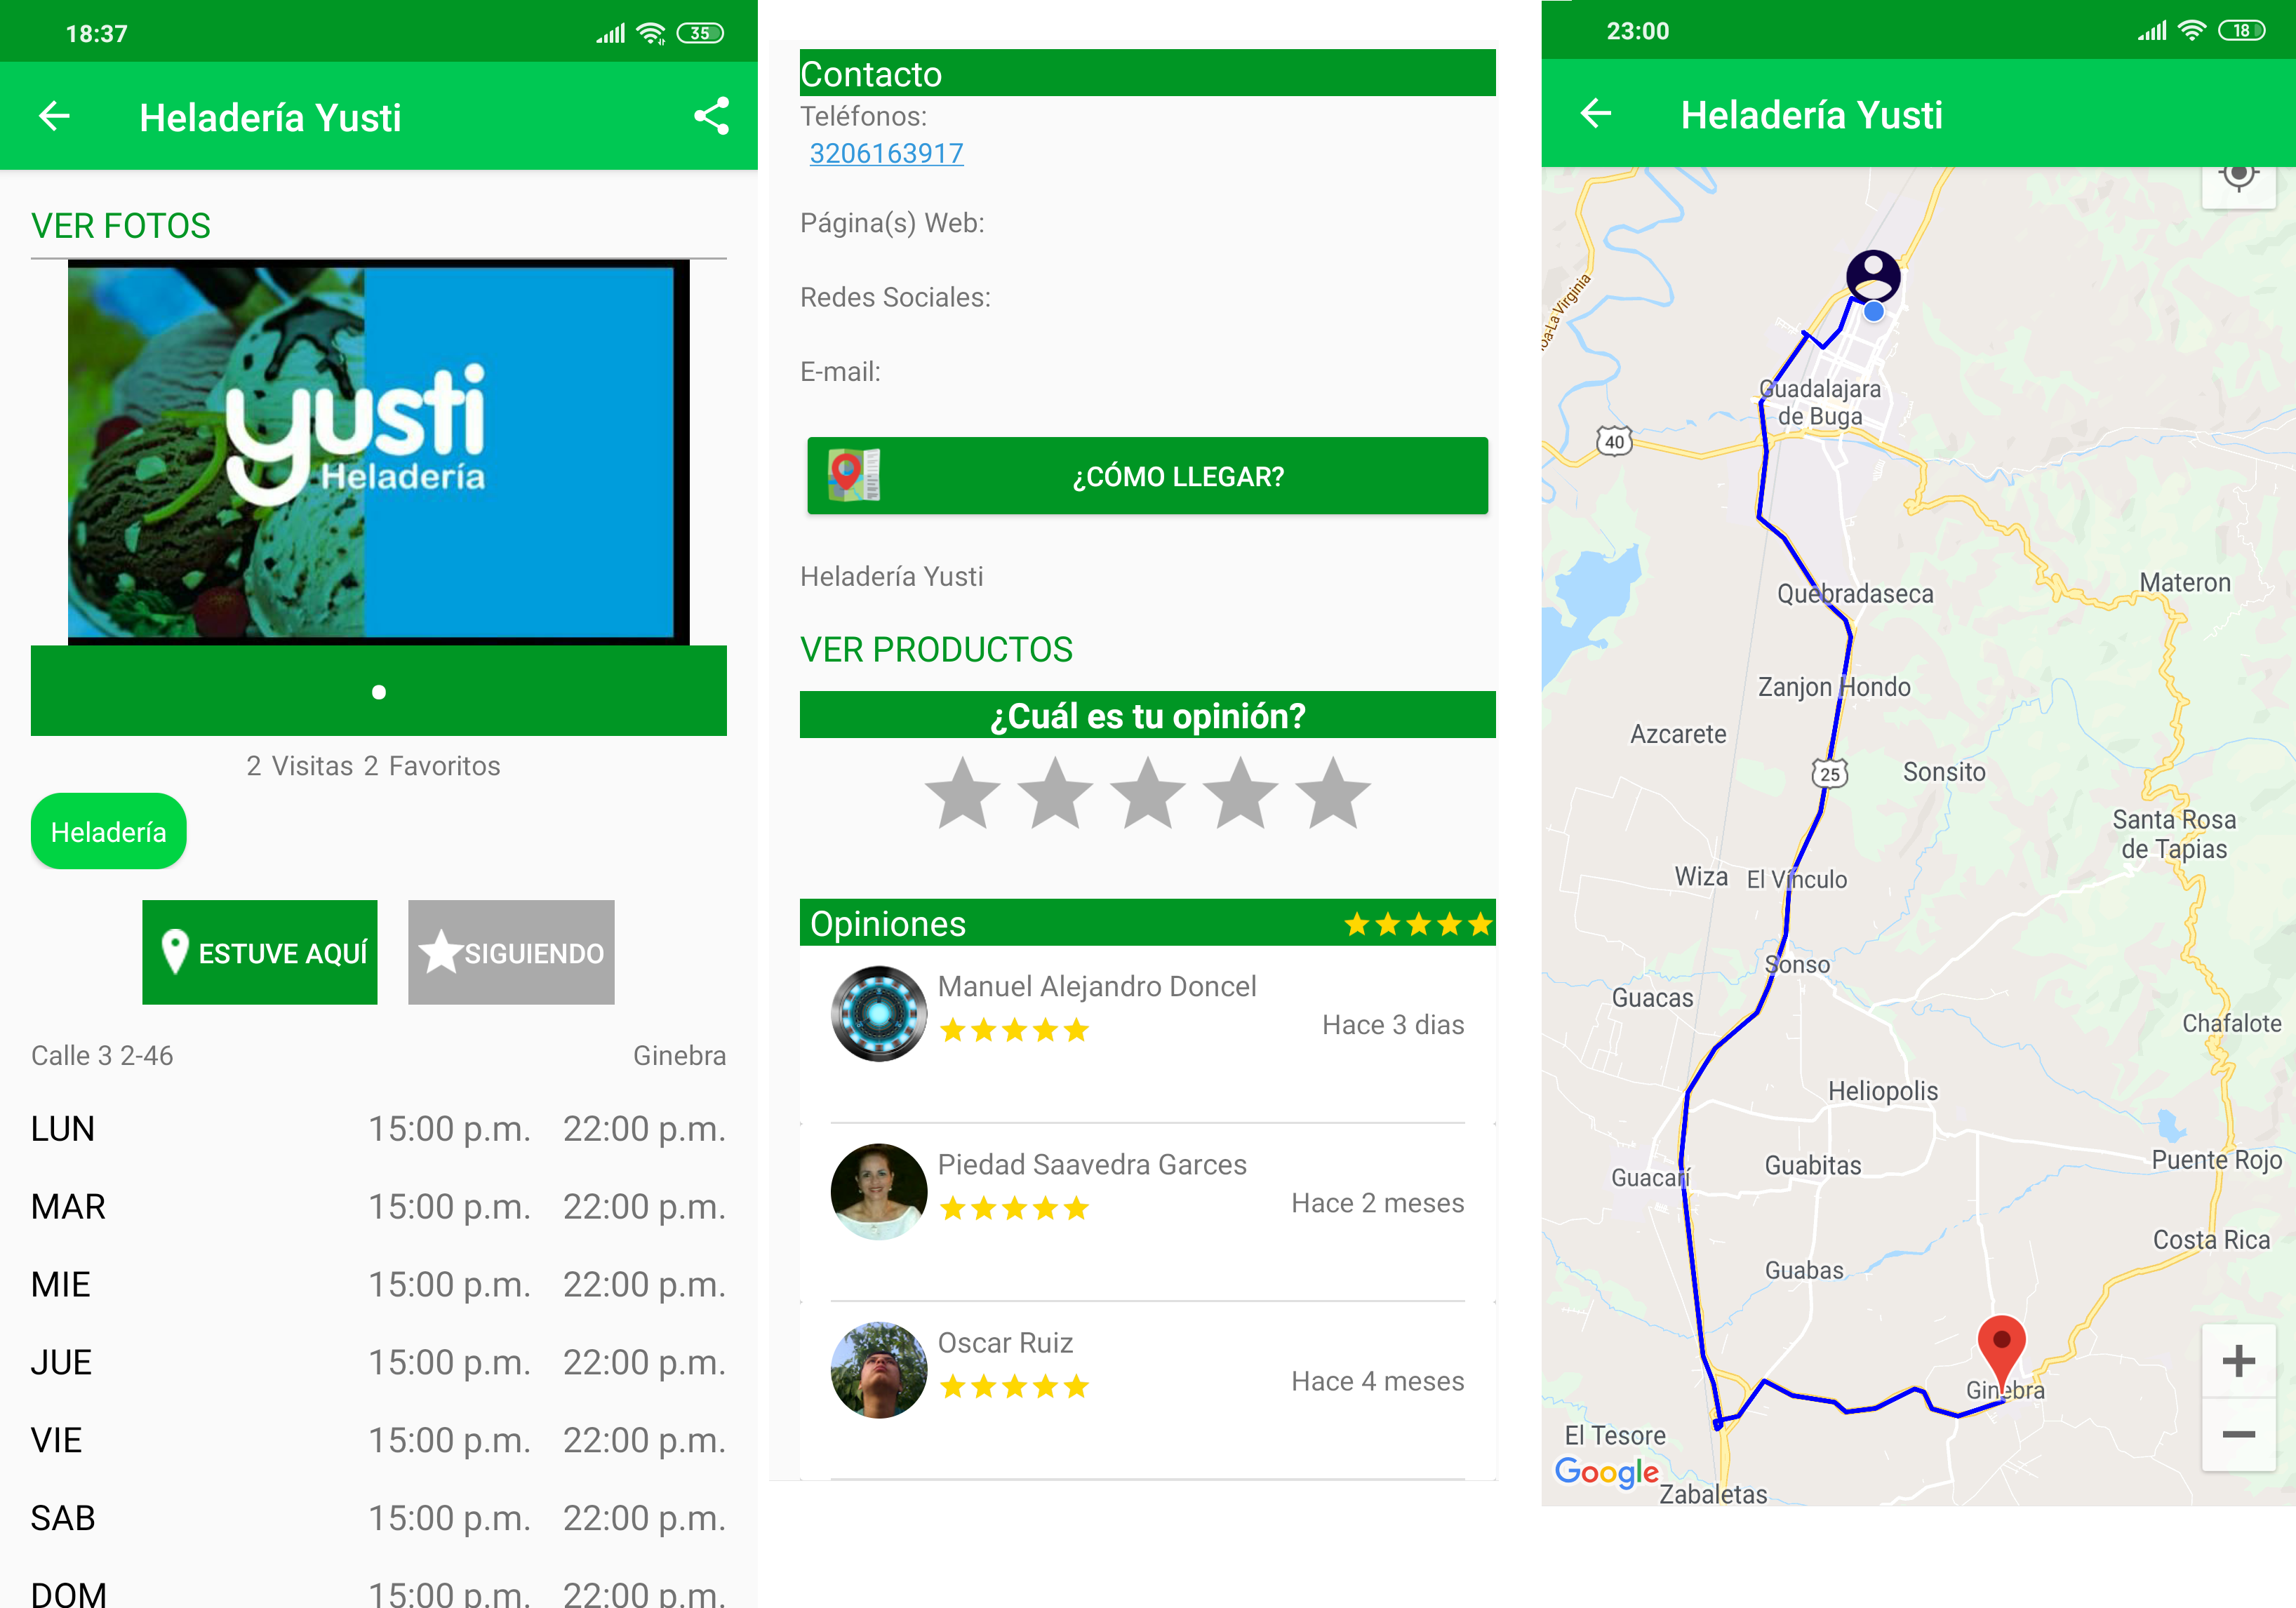
\includegraphics[width=8cm]{./imagenes/4}
\caption{Detalles lugar y ruta/ubicación.}
\end{center}
\end{figure}
Dentro de los detalles de un lugar, es posible realizar una suscripción a este (marcarlo como favorito), registrar una visita por día, y crear un comentario con una calificación.

\subsubsection{Mi perfil}
Dentro de la sección Mi perfil, el usuario podrá visualizar la información referente a él, así como el numero de visitas realizadas, número de  lugares favoritos, número de lugares en propiedad y un listado con la solicitudes realizadas\\
\begin{figure}[H]
\begin{center}
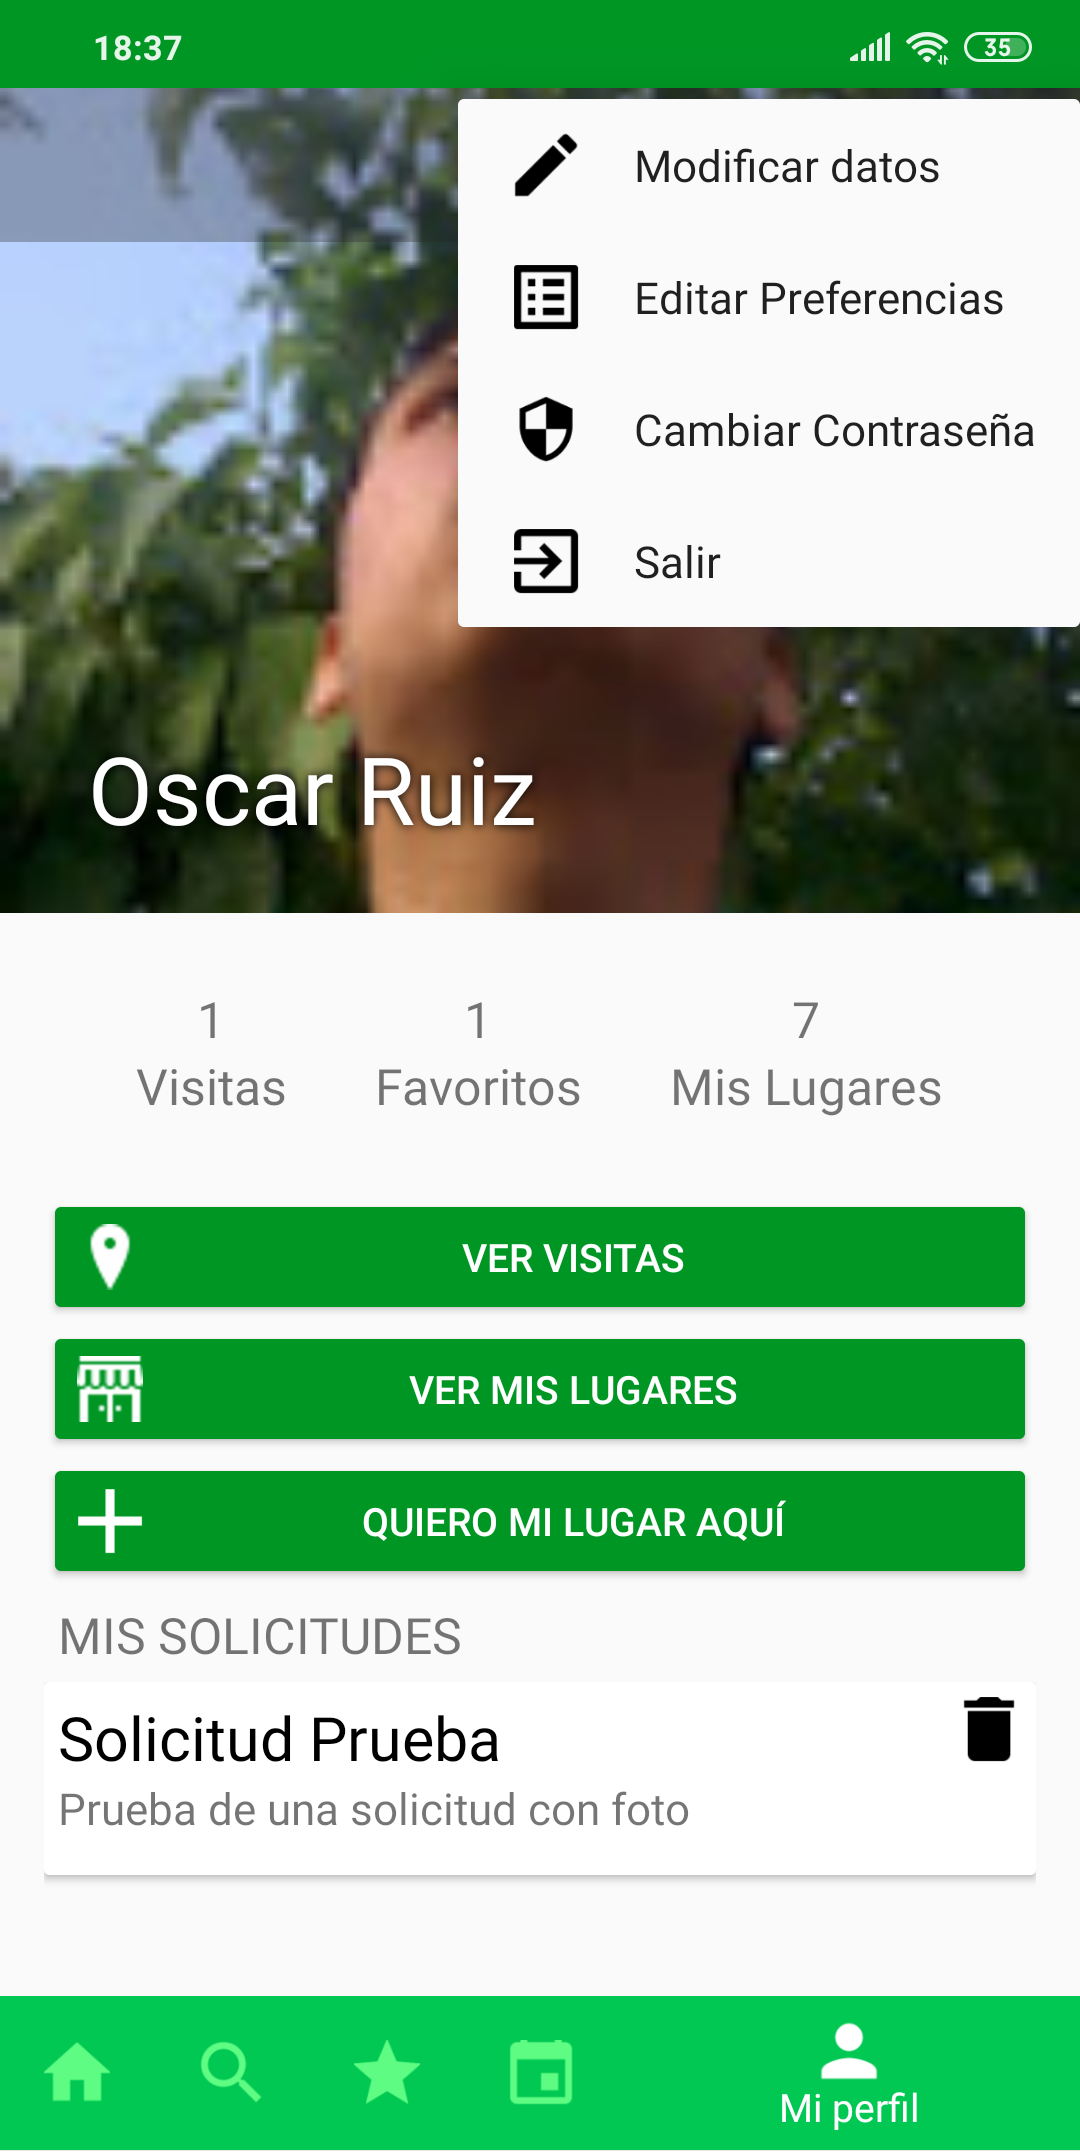
\includegraphics[width=3cm]{./imagenes/5}
\caption{Mi Perfil.}
\end{center}
\end{figure}
También, se brindan opciones para realizar la modificación de datos personales, de contraseña de inicio de sesión, y de preferencias de las cuales recibirá recomendaciones.

\subsubsection{Solicitudes}
Los usuarios pueden realizar solicitudes para registrar su sitio en la aplicación para que sea visible dentro de esta. Las solicitudes se realizan desde la sección Mi Perfil.\\
\begin{figure}[H]
\begin{center}
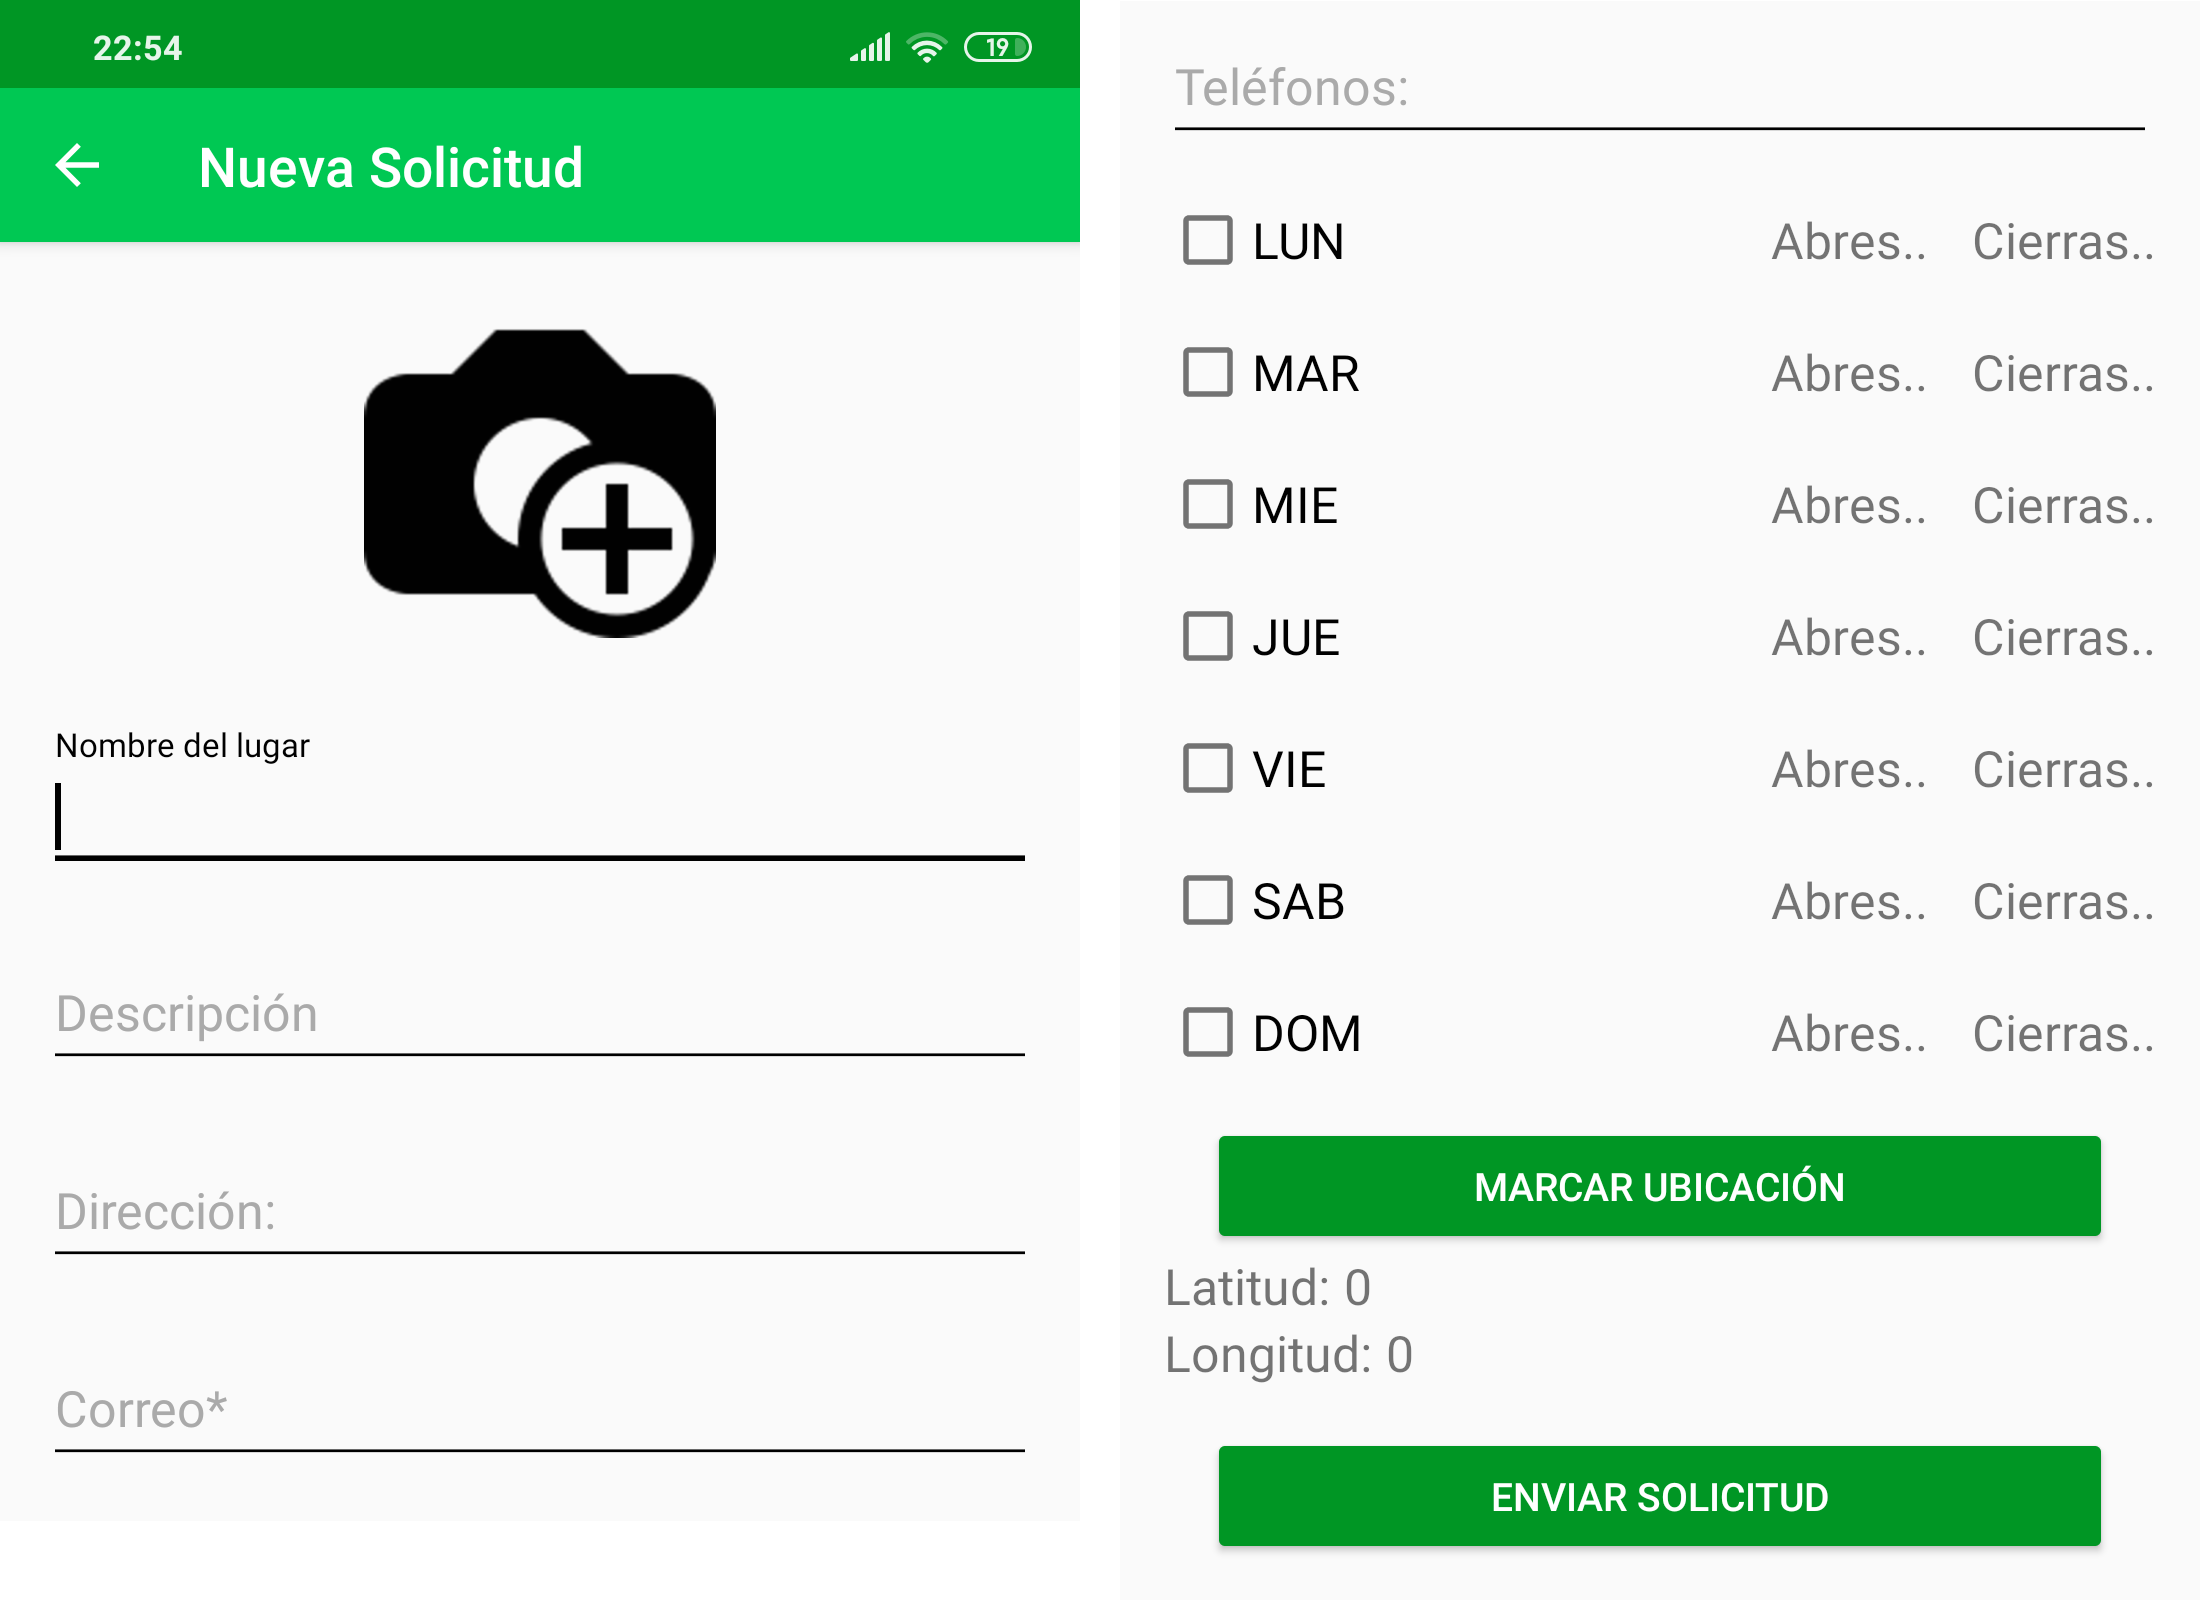
\includegraphics[width=7cm]{./imagenes/6}
\caption{Realizar Solicitud.}
\end{center}
\end{figure}

\subsection{Comerciante}
El usuario tipo comerciante dispone de las mismas funcionalidades de un usuario normal, mencionadas en la sección anterior, pero ademas, el usuario tipo comerciante podrá administrar su negocio, al cual es posible añadirle productos, eventos, y ver los suscriptores a sus lugares.\\
\begin{figure}[H]
\begin{center}
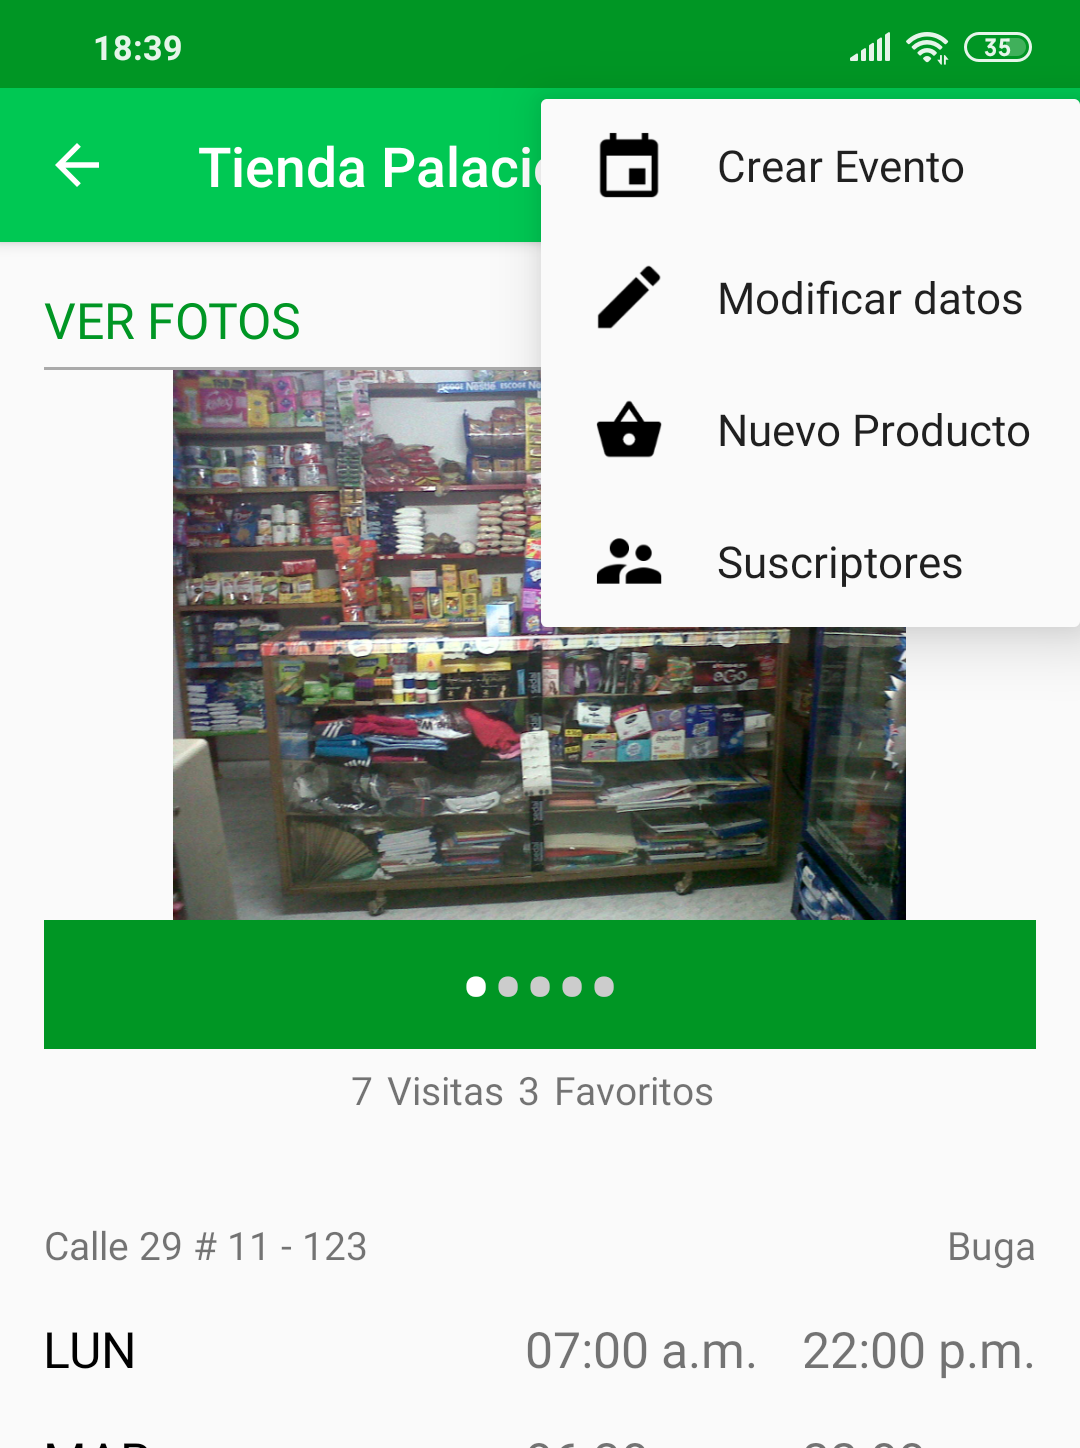
\includegraphics[width=4cm]{./imagenes/7}
\caption{Opciones Lugar Propio.}
\end{center}
\end{figure}

\begin{figure}[H]
    \centering
    \begin{subfigure}{.4\linewidth}
        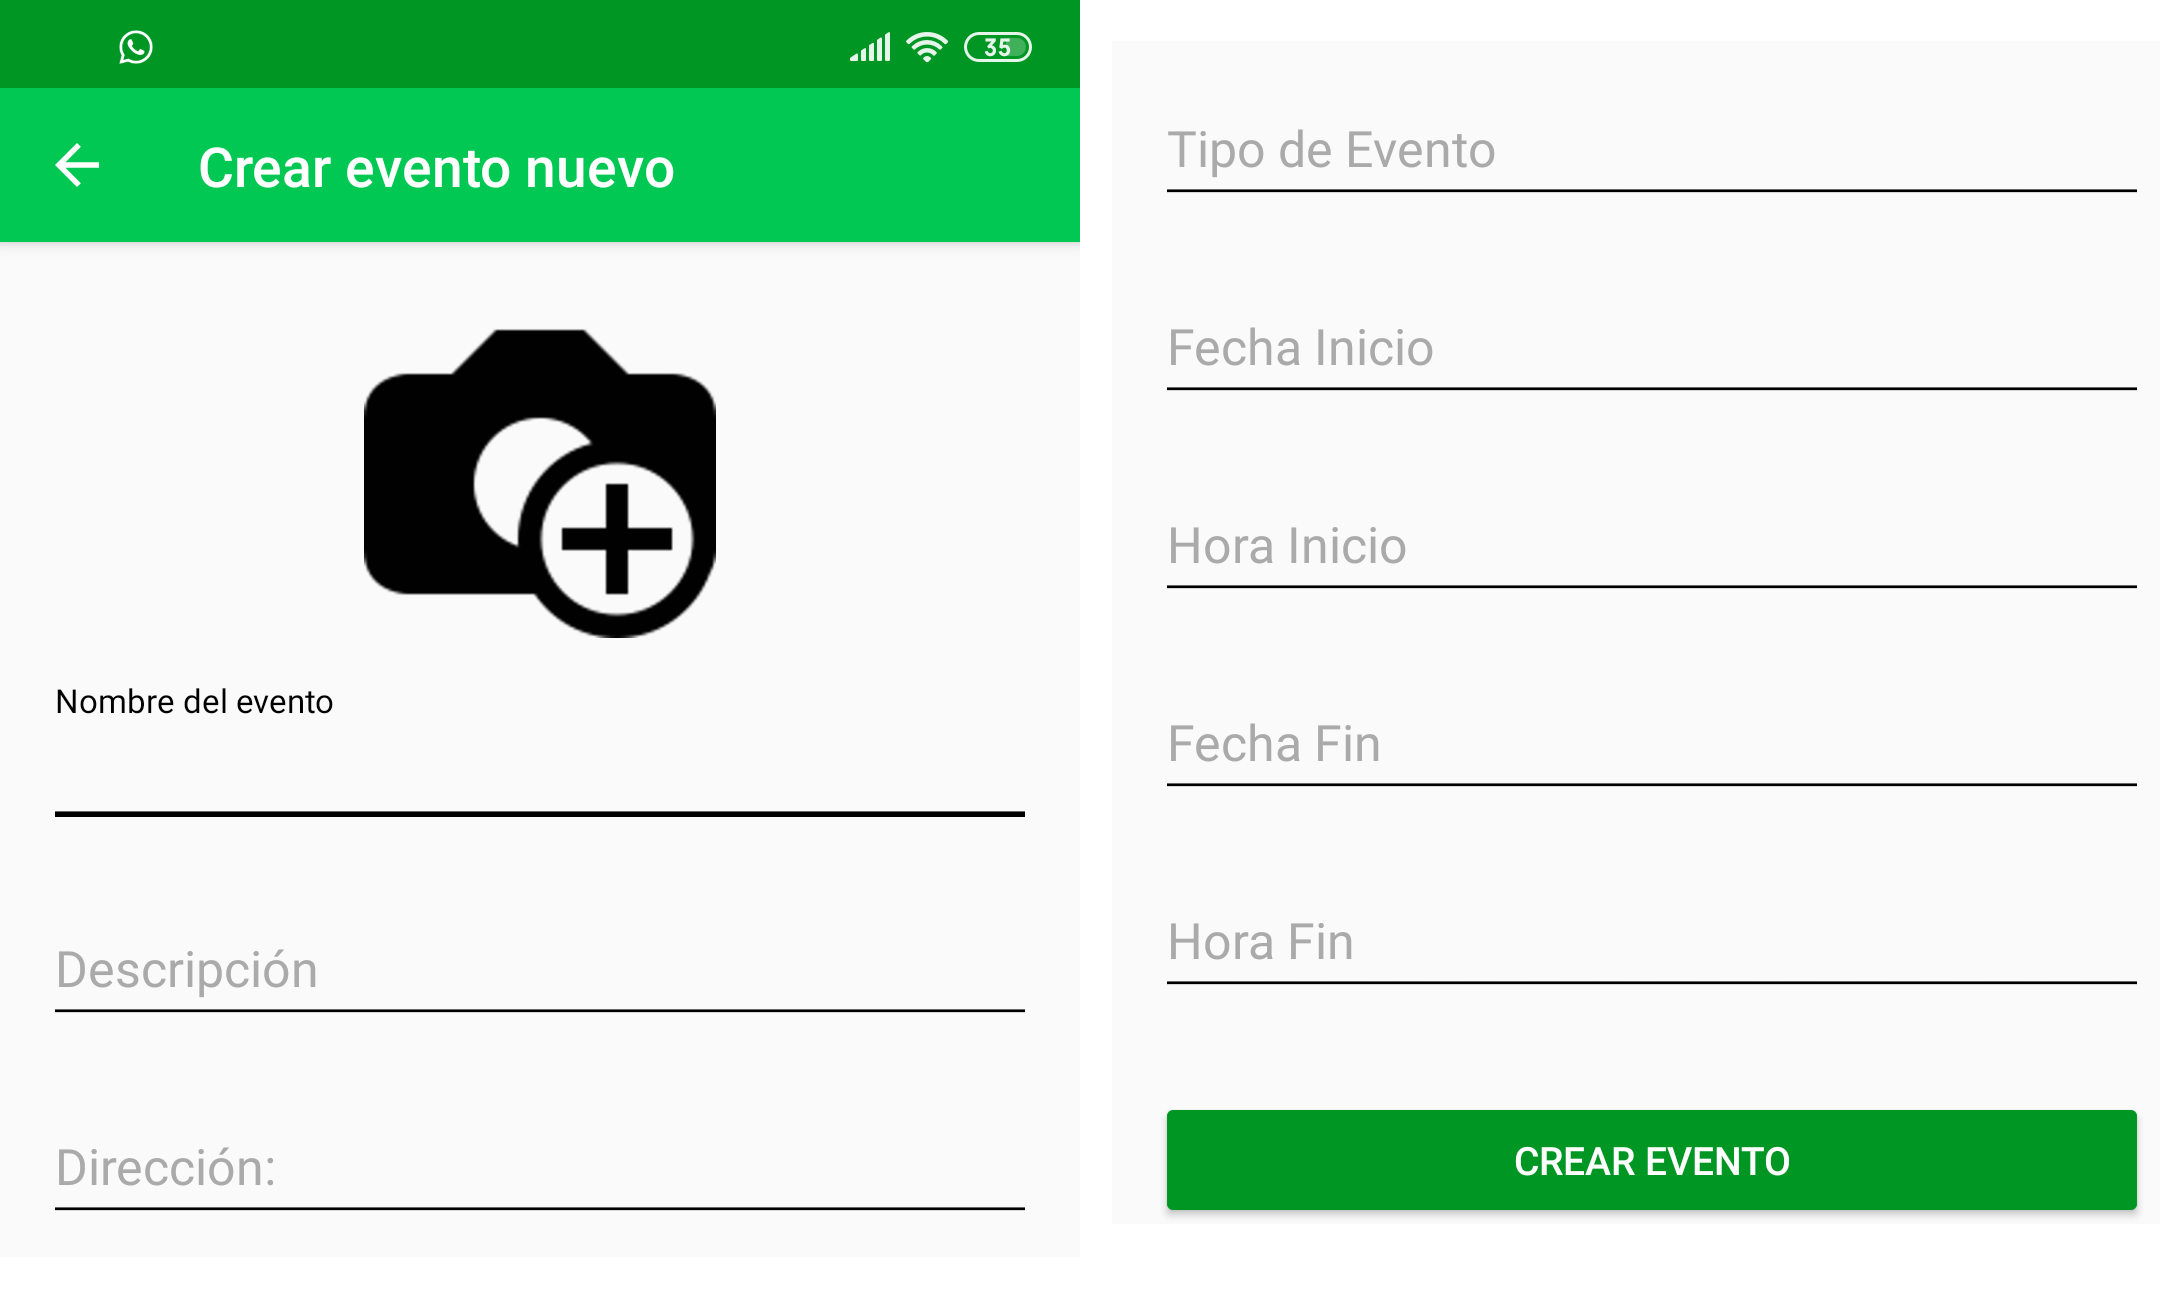
\includegraphics[scale=0.12]{./imagenes/8}
        \caption{Crear Evento.}
    \end{subfigure}
    \hskip2em
    \begin{subfigure}{.4\linewidth}
        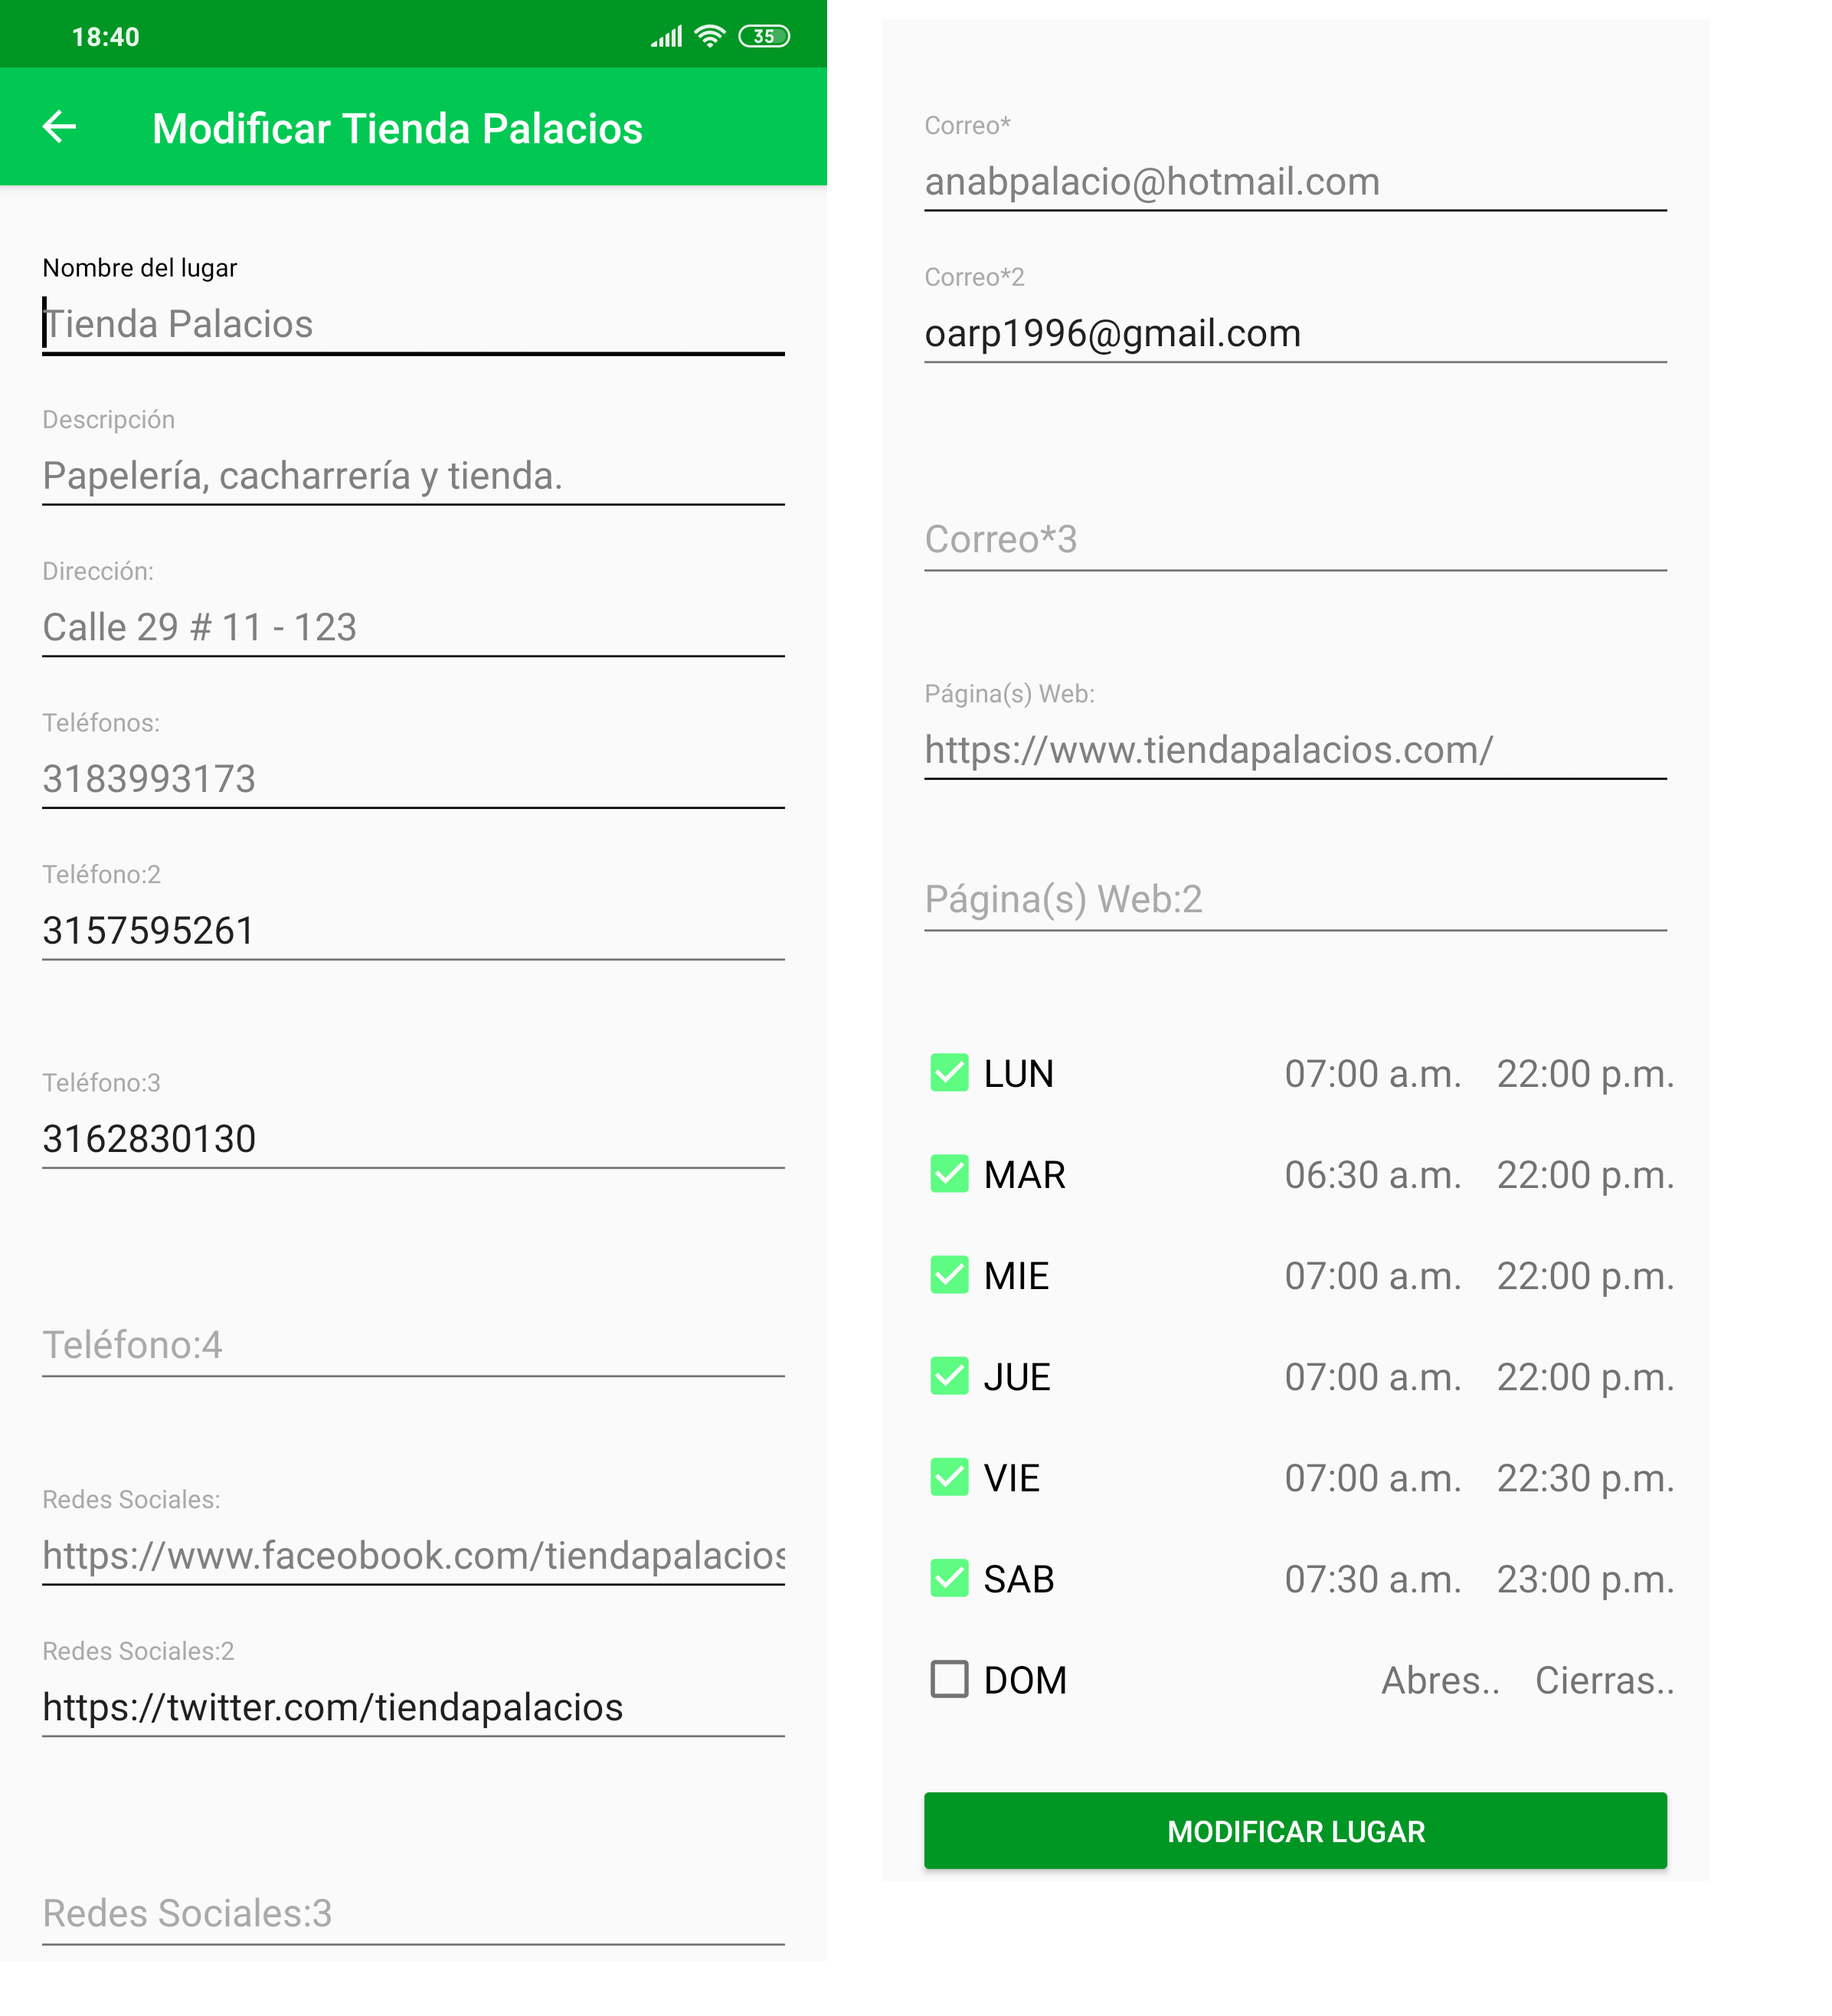
\includegraphics[scale=0.1]{./imagenes/9}
        \caption{Modificar Datos.}
    \end{subfigure}
    \caption{Opciones Comerciante 1}
\end{figure}

\begin{figure}[H]
    \centering
    \begin{subfigure}{.4\linewidth}
        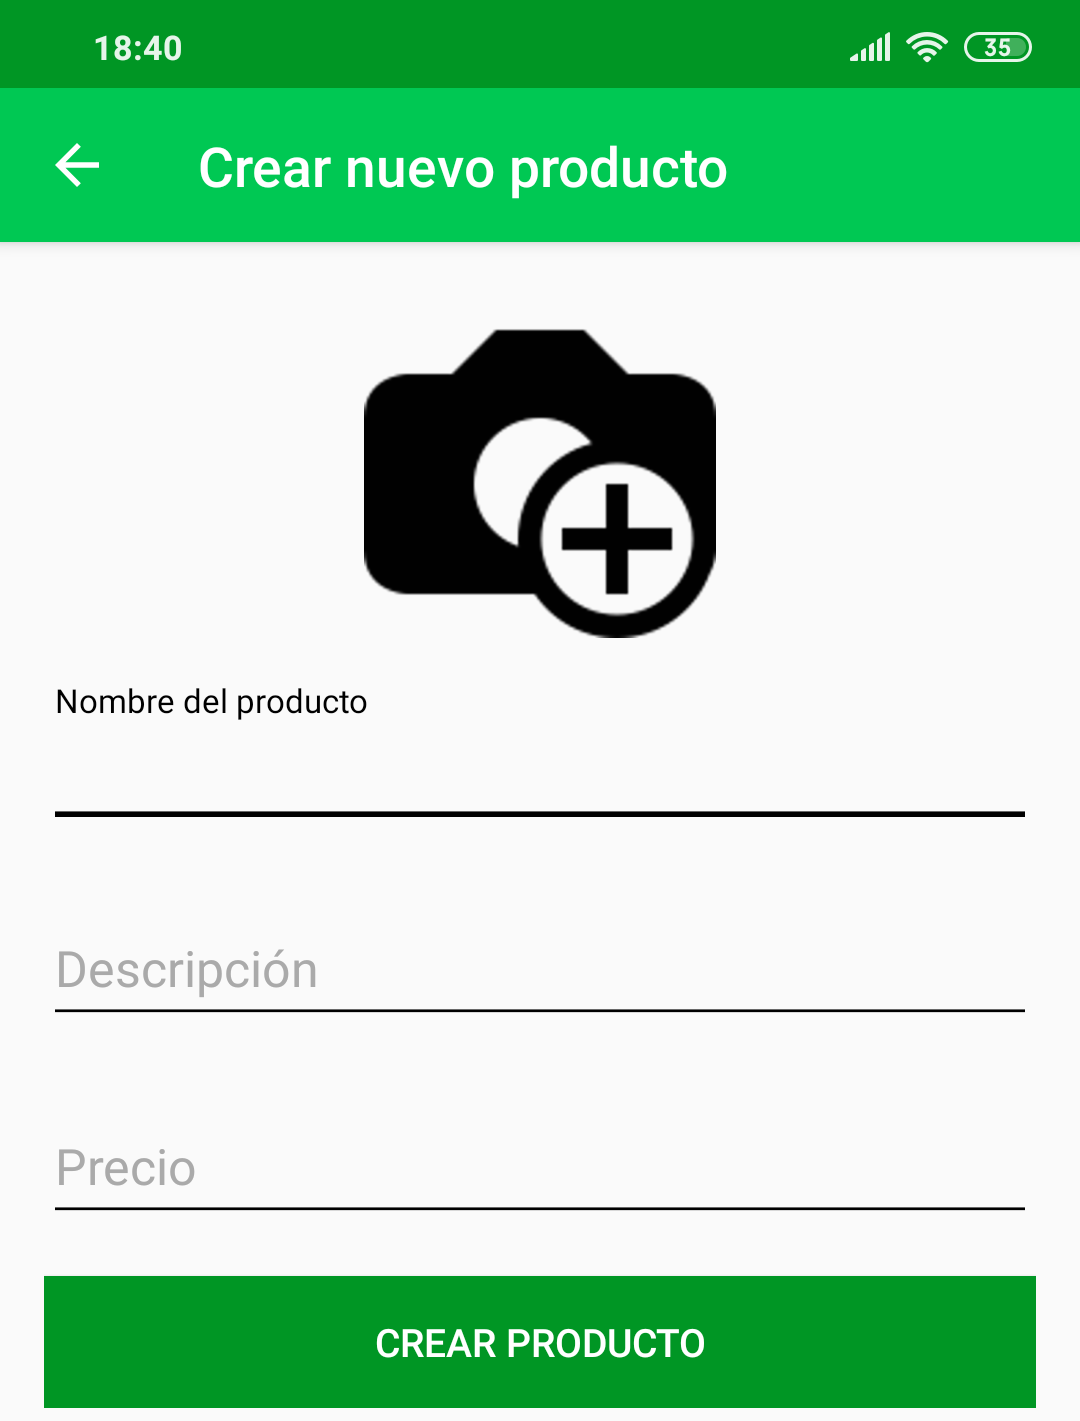
\includegraphics[scale=0.15]{./imagenes/10}
        \caption{Crear Producto.}
    \end{subfigure}
    \hskip2em
    \begin{subfigure}{.4\linewidth}
        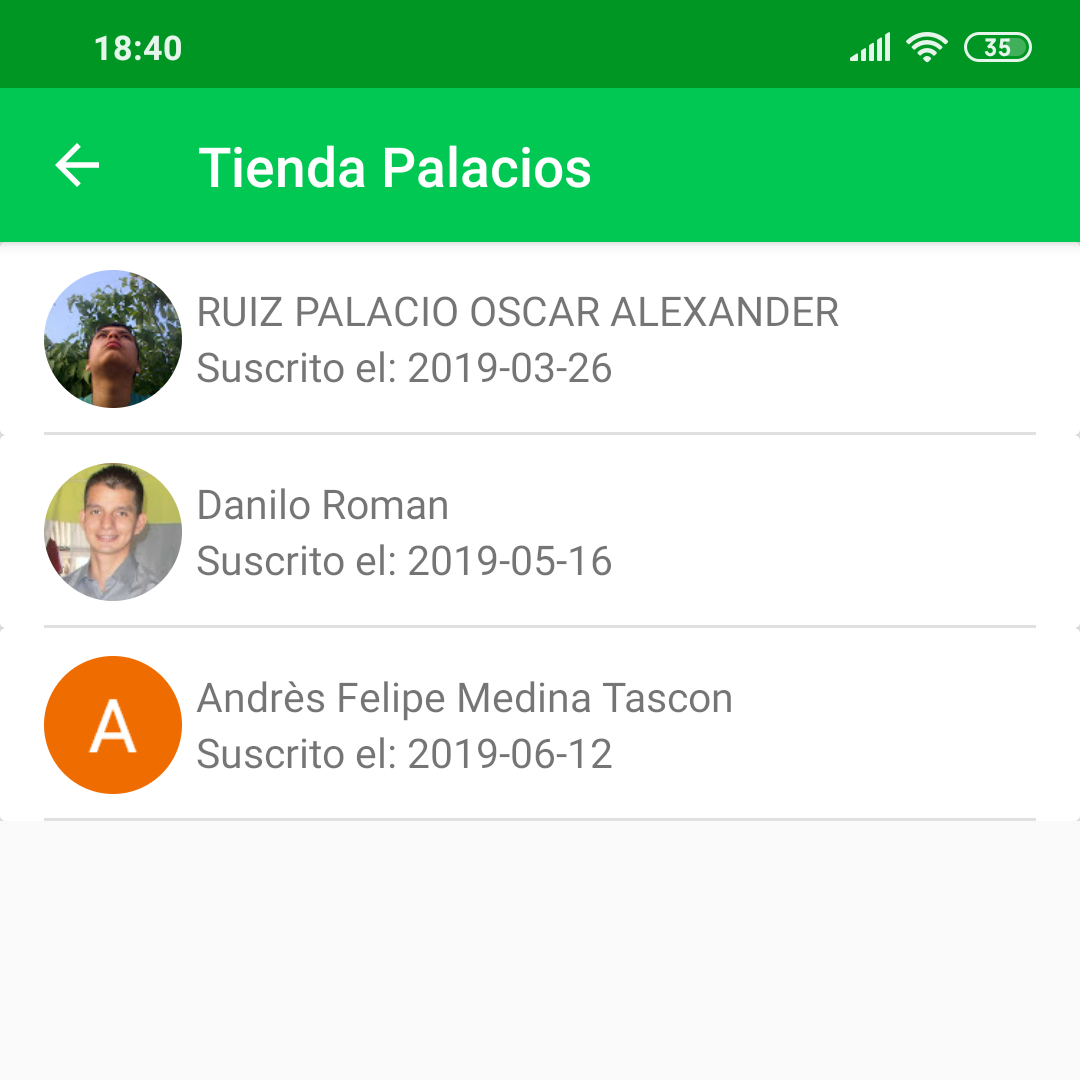
\includegraphics[scale=0.15]{./imagenes/11}
        \caption{Ver Suscriptores.}
    \end{subfigure}
    \caption{Opciones Comerciante 2}
\end{figure}

\section{Detalles de la Implementación}
En un principio se diseñó una encuesta para poder llevar a cabo la caracterización de los sitios \textbf{(Ver Apéndice D)} para lograr el primer objetivo \textbf{(Caracterizar los sitios y eventos del municipio de Ginebra)}, sin embargo, debido a la disponibilidad de los dueños o administradores de estos sitios, está encuesta no pudo ser aplicada en su totalidad formalmente, por lo que fue necesario llevar a cabo la recoleccion de datos a través de un trabajo de campo realizado, y difusión del trabajo por medio de redes sociales.\\
Tanto en el trabajo de campo realizado como en la difusión a través de redes sociales, las preguntas del cuestionario se aplicaron para lograr la recolección de datos.\\
Una vez recolectados los datos, se analizó la información obtenida para extraer aquellos que sea de utilidad para la aplicación, y se alimentó la base de datos con la información de los sitios consultados.
\vspace{5mm}\newline
Para lograr el segundo objetivo \textbf{(Determinar el tipo de sistema de recomendación y los algoritmos a utilizar)}, se realizó una investigación acerca de la funcionalidad y estructura de las técnicas y algoritmos para hacer recomendaciones, y se eligió implementar un Sistema de Recomendación Basado en Contenido, con el algoritmo Vector Space Model (VSM) con ponderación TF-IDF y similitud coseno, ya que es de utilidad para poder analizar datasets pequeños y es conveniente para aplicaciones nuevas, ayudando a evitar problemas de coldstart. El desarrollo de la técnica elegida se puede evidenciar en el \textbf{Apéndice E}.
\vspace{5mm}\newline
Actualmente, se encuentra disponible en versión beta dentro de la Google Play Store, la aplicación movil desarrollada en lenguaje JAVA, la cual tiene como nombre "GuideMe",  teniendo más de 50 descargas, evidencia de este desarrollo se observa en el apartado Diseño y Descripción General del Sistema. De esta manera se logra cumplir con el objetivo \textbf{(Implementar un prototipo de una aplicación móvil que permita consumir y ofrecer la información sobre los sitios y eventos de la ciudad de Ginebra.)}.
\begin{figure}[H]
\begin{center}
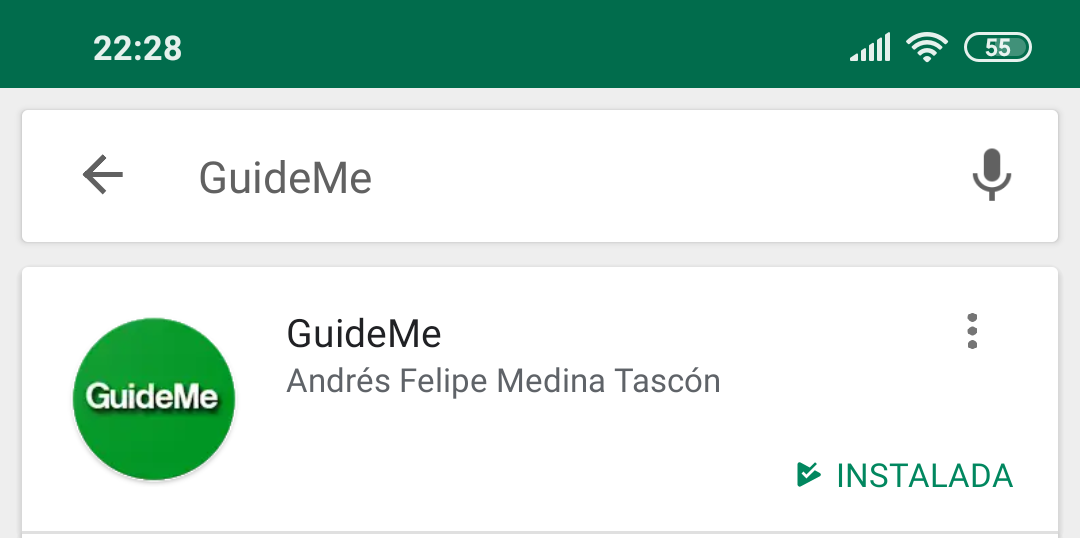
\includegraphics[width=7cm]{./imagenes/gm}
\caption{Aplicación en la Play Store.}
\end{center}
\end{figure}
Videos referentes a la aplicación movil: \\
\url{https://www.youtube.com/watch?v=ihaKEdw0NQM}\\
\url{https://www.youtube.com/watch?v=QLt4tpqouJM}
\vspace{5mm}\newline
Se implementó un prototipo de sistema de recomendación, el cual se encuentra en el Backend dentro del modulo de lugares, para dar cumplimiento al objetivo \textbf{(Implementar un prototipo de sistema de recomendación para los sitios y eventos del municipio de Ginebra.)}. De esta manera, desde la aplicación movil se realiza el llamado a este algoritmo por medio de una petición HTTP GET para poder obtener recomendaciones de acuerdo a las preferencias del usuario y a los tags de los sitios.
\vspace{5mm}\newline
Para lograr el quinto objetivo \textbf{(Evaluar las recomendaciones emitidas por el sistema de recomendación conforme a la realimentación de los usuarios de la aplicación.)}, se hizo de la siguiente manera:\\
El sistema de recomendación lanza una predicción, la cual es un valor que va de 0 a 1, mientras el valor sea mayor a 0, se muestra como una recomendación, sin embargo, en la evaluación, se toma un valor de 0.35 en adelante para considerarlo como recomendado. \\
Se evaluaron las recomendaciones con  los datos recogidos gracias a los habitantes de Ginebra y con colaboración de los estudiantes de la Universidad del Valle sede Tuluá, de los cuales se obtuvieron 81 registros, y, de esta manera, se obtuvieron los siguientes resultados:
\begin{table}[H]
\centering
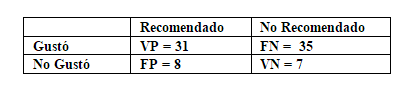
\includegraphics[width=10cm]{./imagenes/PrecisionRecall}
\caption{Matriz de Confusión.}
\end{table}

Un verdadero positivo es un resultado en el que el modelo predice correctamente la clase positiva. De manera similar, un verdadero negativo es un resultado en el que el modelo predice correctamente la clase negativa.\\
Un falso positivo es un resultado en el que el modelo predice incorrectamente la clase positiva. Y un falso negativo es un resultado en el que el modelo predice incorrectamente la clase negativa.\\
La precisión intenta responder a la siguiente pregunta: ¿Qué proporción de identificaciones positivas fue correcta?\\
La exhaustividad intenta responder a la siguiente pregunta: ¿Qué proporción de positivos reales se identificó correctamente?\cite{13}\cite{26}
\vspace{5mm}\newline
Precisión = $\frac{VP}{VP+FP}$ = 0.79 \\
Recall = $\frac{VP}{VP+FN}$ = 0.47\\
\newline
Se obtuvo una precisión de 0.79, por que el 79\% de las recomendaciones fueron de agrado para los usuarios, y se obtuvo una exhaustividad de 0.47, por lo que recomienda el 47\% lugares que les gustan a los usuarios
\vspace{5mm}\newline
Por otro lado, \textbf{las tecnologías usadas en el desarrollo del proyecto fueron:}
\begin{itemize}
    \item Android: Android \cite{27} es un sistema operativo móvil desarrollado por Google, basado en el Kernel de Linux y otros software de código abierto.
    \item Java: Java \cite{28} es un lenguaje de programación de propósito general, concurrente y orientado a objetos.
    \item Python: Python \cite{29} es un lenguaje de programación interpretado, usa tipado dinámico y es multiplataforma.
    \item PostgreSQL: PostgreSQL \cite{30} es un motor de base de datos libre, robusto y proporciona buenos niveles de seguridad.
    \item Django: Django \cite{31} es un framework de aplicaciones web de alto nivel que fomenta el desarrollo rápido y el diseño limpio y pragmático.
    \item ReactJS: React \cite{32} es una biblioteca Javascript para crear interfaces de usuario.
    \item Scikit-learn: Scikit-learn \cite{33} es una biblioteca para machine learning, para el lenguaje de programación Python.
    \item Numpy: Numpy \cite{34} es una extensión de Python, que le agrega mayor soporte para vectores y matrices, constituyendo una biblioteca de funciones matemáticas de alto nivel para operar con esos vectores o matrices.
    \item Firebase: Firebase \cite{35} es una plataforma para el desarrollo de aplicaciones web y aplicaciones móviles.
    \item Pusher: Pusher \cite{36} permite a los desarrolladores con APIs crear funciones de colaboración y comunicación en sus aplicaciones web y móviles.
\end{itemize}

\section{Pruebas}
Las pruebas realizadas para verificar el correcto comportamiento del sistema fueron pruebas funcionales, pruebas unitarias, pruebas de usabilidad y pruebas de precision and recall. Ademas, informe de errores y funcionalidad de la aplicación móvil en distintos emuladores móviles que presta la herramienta de Google.

\subsection{Pruebas de la tienda de aplicación}
\begin{figure}[H]
\begin{center}
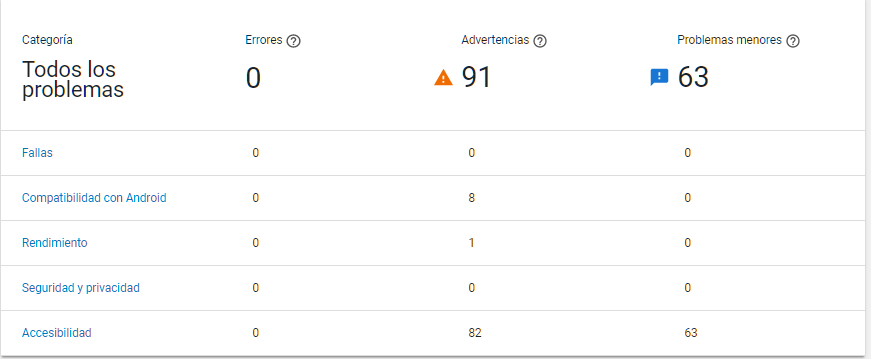
\includegraphics[width=10cm]{./imagenes/Test/Informe_errores_play_store}
\caption{Informe Errores Play Store.}
\end{center}
\end{figure}

\begin{figure}[H]
\begin{center}
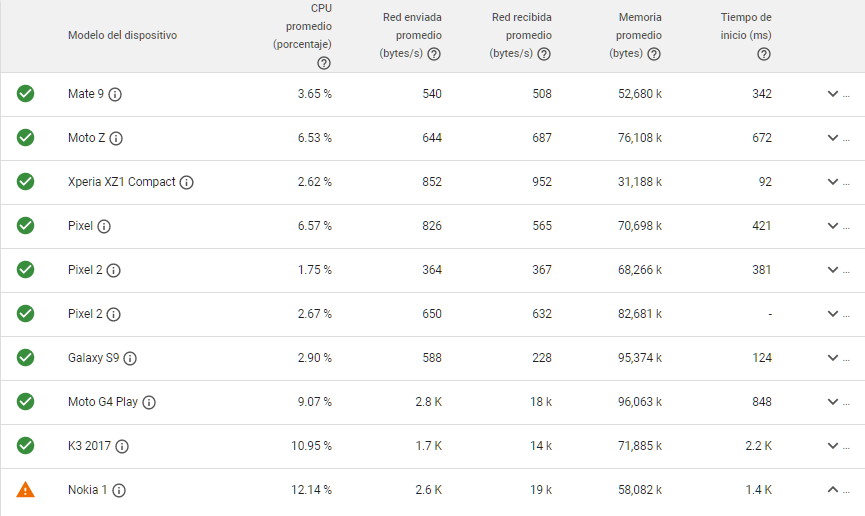
\includegraphics[width=10cm]{./imagenes/Test/Informe_movile_play_console}
\caption{Informe Móvil Play Store.}
\end{center}
\end{figure}

\subsection{Pruebas Funcionales}
\begin{table}[H]
\centering
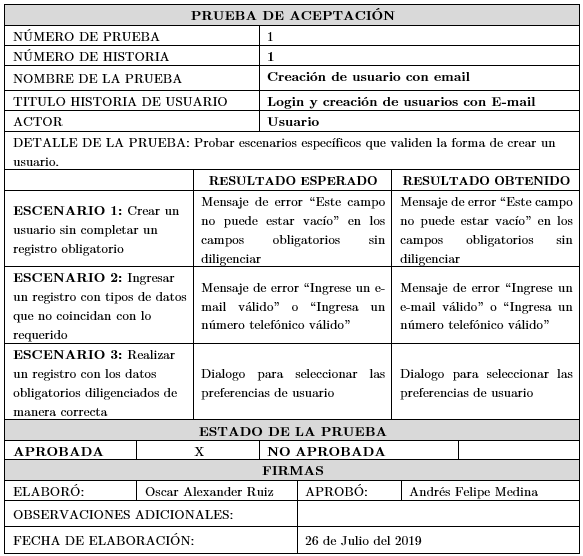
\includegraphics[width=8cm]{./imagenes/PA/PA1}
\caption{PA1: Creación de usuario con email.}
\end{table}

\begin{table}[H]
\centering
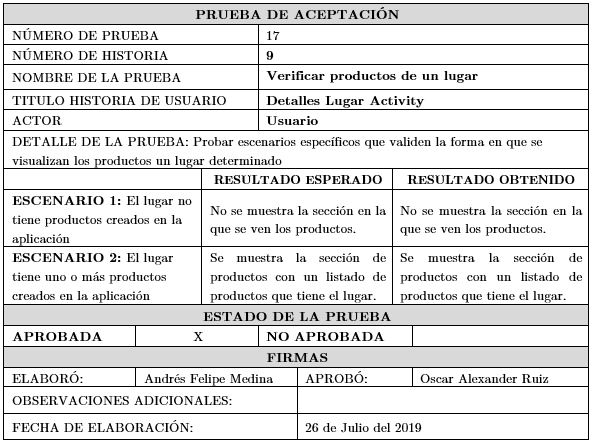
\includegraphics[width=8cm]{./imagenes/PA/PA17}
\caption{PA17: Verificar productos de un lugar.}
\end{table}

\begin{table}[H]
\centering
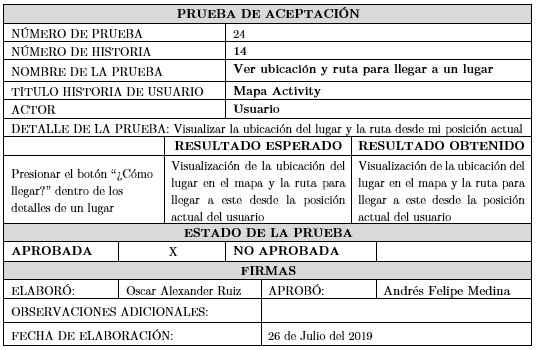
\includegraphics[width=8cm]{./imagenes/PA/PA24}
\caption{PA24: Ver ubicación y ruta para llegar a un lugar.}
\end{table}

Las demás pruebas funcionales realizadas las puede detallar en el documento Anexo, Apéndice E.

\subsection{Pruebas Unitarias}
\begin{figure}[H]
\begin{center}
\includegraphics[width=10cm]{./imagenes/Test/ControladorFechasTest}
\caption{Prueba Unitaria Método Controlador Fechas App Movil.}
\end{center}
\end{figure}

\begin{figure}[H]
\begin{center}
\includegraphics[width=6cm]{./imagenes/Test/Backend/Test__lugares_api_test}
\caption{Prueba Unitaria Modulo Lugar - Backend.}
\end{center}
\end{figure}

Los demás pruebas unitarias realizadas las puede detallar en el documento Anexo, Apéndice E.

\subsection{Prueba de Usabilidad}
\begin{figure}[H]
\begin{center}
\includegraphics[width=11cm]{./imagenes/R1}
\caption{Evaluación heurística para aplicación móvil P1.}
\end{center}
\end{figure}

\begin{figure}[H]
\begin{center}
\includegraphics[width=11cm]{./imagenes/R2}
\caption{Evaluación heurística para aplicación móvil P2.}
\end{center}
\end{figure}
%%%%%%%%%%%%%%%%%%%%%%%%%%%%%%%%%%%%%%%%%%%%%%%%%%%%%%%%%%%%%%%%%%%%%%%%%%%%%%%%%%%%%%%%%%
%%%%%%%%%%%%%%%%%%%%%%%%%%%%%%						FIN DESARROLLO DEL PROYECTO
%%%%%%%%%%%%%%%%%%%%%%%%%%%%%%%%%%%%%%%%%%%%%%%%%%%%%%%%%%%%%%%%%%%%%%%%%%%%%%%%%%%%%%%%%%

%%%%%%%%%%%%%%%%%%%%%%%%%%%%%%%%%%%%%%%%%%%%%%%%%%%%%%%%%%%%%%%%%%%%%%%%%%%%%%%%%%%%%%%%%%%%%%%%%%
%%%%%%%%%%%%%%%%%%%%%%%%%%%%%%%%%%%%%%%%%%%%%%%%%%%%%%%%%%%%%%%%%%%%%%%%%%%%%%%%%%%%%%%%%%%%%%%%%%
%%%%%%%%%%%%%%%%%%%%%%%%%%%%%%%%%%%%%%%%%%%%%%%%%%%%%%%%%%%%%%%%%%%%%%%%%%%%%%%%%%%%%%%%%%%%%%%%%%
%%%%%%%%%%%%%%%%%%%%%%%%%%%%%%%%%%%%%%%%%%%%%%%%%%%%%%%%%%%%%%%%%%%%%%%%%%%%%%%%%%%%%%%%%%%%%%%%%%

%%%%%%%%%%%%%%%%%%%%%%%%%%%%%%%%%%%%%%%%%%%%%%%%%%%%%%%%%%%%%%%%%%%%%%%%%%%%%%%%%%%%%%%%%%
%%%%%%%%%%%%%%%%%%%%%%%%%%%%%%						CONCLUSIONES Y TRABAJO FUTURO
%%%%%%%%%%%%%%%%%%%%%%%%%%%%%%%%%%%%%%%%%%%%%%%%%%%%%%%%%%%%%%%%%%%%%%%%%%%%%%%%%%%%%%%%%%
\chapter{Conclusiones y Trabajos Futuros}\label{cap.conclu_trabajos}
\section{Conclusiones}
\begin{itemize}
    \item Se encontró una ausencia de datos respecto a los diferentes sitios del municipio de
Ginebra, por lo cual fue necesario realizar un trabajo de campo para actualizar los
datos de los sitios nuevos del municipio y actualizar los ya existentes de los establecimientos que permitieron realizar esta labor.\\
Ademas, debido a la falta de disponibilidad de las personas administradoras de algunos de los sitios consultados, fue necesario contactar estas mediante sus redes sociales.
\item La mejor opción para el sistema de recomendación implementada fue VSM, ya que evita el coldstart y puede hacer recomendaciones de lugares a los usuarios en su primer ingreso, además de que tiene un costo computacional razonable para el proyecto que se realizó.
\item Haciendo uso de la metodología Mobile-D, y a los conocimientos adquiridos a lo largo de los años académicos en la Universidad sobre el lenguaje de programación JAVA, se logró implementar la aplicación móvil en el tiempo estipulado para el desarrollo del trabajo.
\item Se desarrolló una aplicación web para que la administración de la aplicación pueda ser realizada no necesariamente por una persona experta.
   \item Al obtener una precisión del 79\%, se puede concluir que las recomendaciones generadas fueron de agrado para los usuarios, sin embargo, al tener un recall del 47\%, no se están tomando en cuenta todos los sitios que podrían llegar a gustar a los usuarios.
\end{itemize}


\section{Trabajo Futuro}
\begin{itemize}
\item Una vez la aplicación posea mayor cantidad de datos, se puede realizar un estudio más a fondo, con el objetivo de complementar el enfoque del sistema de recomendación basado en contenido, por un sistema de recomendación basado en filtrado colaborativo, ya que un sistema de recomendación basado en contenido presenta problemas sobre especialización y no puede brindar diversidad en las recomendaciones, un aspecto que es importante en las recomendaciones para el sector turístico.
\item Expandir el alcance de la aplicación móvil para que contenga sitios característicos de otros municipios.
\item Desarrollar una aplicación en iOS para dispositivos Apple.
\item Complementar la aplicación web, para permitir le consumo de la información de los sitios.
\end{itemize}
%%%%%%%%%%%%%%%%%%%%%%%%%%%%%%%%%%%%%%%%%%%%%%%%%%%%%%%%%%%%%%%%%%%%%%%%%%%%%%%%%%%%%%%%%%
%%%%%%%%%%%%%%%%%%%%%%%%%%%%%%						FIN CONCLUSIONES Y TRABAJO FUTURO
%%%%%%%%%%%%%%%%%%%%%%%%%%%%%%%%%%%%%%%%%%%%%%%%%%%%%%%%%%%%%%%%%%%%%%%%%%%%%%%%%%%%%%%%%%

%%%%%%%%%%%%%%%%%%%%%%%%%%%%%%%%%%%%%%%%%%%%%%%%%%%%%%%%%%%%%%%%%%%%%%%%%%%%%%%%%%%%%%%%%%%%%%%%%%
%%%%%%%%%%%%%%%%%%%%%%%%%%%%%%%%%%%%%%%%%%%%%%%%%%%%%%%%%%%%%%%%%%%%%%%%%%%%%%%%%%%%%%%%%%%%%%%%%%
%%%%%%%%%%%%%%%%%%%%%%%%%%%%%%%%%%%%%%%%%%%%%%%%%%%%%%%%%%%%%%%%%%%%%%%%%%%%%%%%%%%%%%%%%%%%%%%%%%
%%%%%%%%%%%%%%%%%%%%%%%%%%%%%%%%%%%%%%%%%%%%%%%%%%%%%%%%%%%%%%%%%%%%%%%%%%%%%%%%%%%%%%%%%%%%%%%%%%

%%%%%%%%%%%%%%%%%%%%%%%%%%%%%%%%%%%%%%%%%%%%%%%%%%%%%%%%%%%%%%%%%%%%%%%%%%%%%%%%%%%%%%%%%%
%%%%%%%%%%%%%%%%%%%%%%%%%%%%%%						APENDICE A
%%%%%%%%%%%%%%%%%%%%%%%%%%%%%%%%%%%%%%%%%%%%%%%%%%%%%%%%%%%%%%%%%%%%%%%%%%%%%%%%%%%%%%%%%%
\appendix
\chapter{Historias de Usuario}\label{aped.A}
En este anexo se relaciona parte de las Historias de Usuario (HU) que fueron necesarias para el desarrollo de este proyecto.	
\begin{table}[H]
\centering
\includegraphics[width=9cm]{./imagenes/HU/HU2}
\caption{HU2: Login y creación de usuarios con Google.}
\end{table}

\begin{table}[H]
\centering
\includegraphics[width=9cm]{./imagenes/HU/HU3}
\caption{HU3: Home Fragment.}
\end{table}

\begin{table}[H]
\centering
\includegraphics[width=9cm]{./imagenes/HU/HU4}
\caption{HU4: Search Fragment.}
\end{table}

\begin{table}[H]
\centering
\includegraphics[width=9cm]{./imagenes/HU/HU5}
\caption{HU5: Favorite Fragment.}
\end{table}

\begin{table}[H]
\centering
\includegraphics[width=9cm]{./imagenes/HU/HU6}
\caption{HU6: Evento Fragment.}
\end{table}

\begin{table}[H]
\centering
\includegraphics[width=9cm]{./imagenes/HU/HU7}
\caption{HU7: Profile Fragment.}
\end{table}

\begin{table}[H]
\centering
\includegraphics[width=9cm]{./imagenes/HU/HU8}
\caption{HU8: Solicitud.}
\end{table}

\begin{table}[H]
\centering
\includegraphics[width=9cm]{./imagenes/HU/HU10}
\caption{HU10: Opciones Detalles Lugar Activity.}
\end{table}

\begin{table}[H]
\centering
\includegraphics[width=9cm]{./imagenes/HU/HU11}
\caption{HU11: Detalles Evento Activity.}
\end{table}

\begin{table}[H]
\centering
\includegraphics[width=9cm]{./imagenes/HU/HU12}
\caption{HU12: Opciones Detalles Evento Activity.}
\end{table}

\begin{table}[H]
\centering
\includegraphics[width=9cm]{./imagenes/HU/HU13}
\caption{HU13: Detalles Producto Activity.}
\end{table}

\begin{table}[H]
\centering
\includegraphics[width=9cm]{./imagenes/HU/HU15}
\caption{HU15: Mapa Categoria Activity.}
\end{table}

\begin{table}[H]
\centering
\includegraphics[width=9cm]{./imagenes/HU/HU16}
\caption{HU16: Crear Evento Activity.}
\end{table}

\begin{table}[H]
\centering
\includegraphics[width=9cm]{./imagenes/HU/HU17}
\caption{HU17: Modificar Evento Activity.}
\end{table}

\begin{table}[H]
\centering
\includegraphics[width=9cm]{./imagenes/HU/HU18}
\caption{HU18: Crear Producto Activity.}
\end{table}

\begin{table}[H]
\centering
\includegraphics[width=9cm]{./imagenes/HU/HU19}
\caption{HU19: Modificar Producto Activity.}
\end{table}

\begin{table}[H]
\centering
\includegraphics[width=9cm]{./imagenes/HU/HU20}
\caption{HU20: Modificar Lugar Activity.}
\end{table}

\begin{table}[H]
\centering
\includegraphics[width=9cm]{./imagenes/HU/HU21}
\caption{HU21: Preferencias.}
\end{table}
%%%%%%%%%%%%%%%%%%%%%%%%%%%%%%%%%%%%%%%%%%%%%%%%%%%%%%%%%%%%%%%%%%%%%%%%%%%%%%%%%%%%%%%%%%
%%%%%%%%%%%%%%%%%%%%%%%%%%%%%%						FIN APENDICE A
%%%%%%%%%%%%%%%%%%%%%%%%%%%%%%%%%%%%%%%%%%%%%%%%%%%%%%%%%%%%%%%%%%%%%%%%%%%%%%%%%%%%%%%%%%

%%%%%%%%%%%%%%%%%%%%%%%%%%%%%%%%%%%%%%%%%%%%%%%%%%%%%%%%%%%%%%%%%%%%%%%%%%%%%%%%%%%%%%%%%%
%%%%%%%%%%%%%%%%%%%%%%%%%%%%%%						APENDICE B
%%%%%%%%%%%%%%%%%%%%%%%%%%%%%%%%%%%%%%%%%%%%%%%%%%%%%%%%%%%%%%%%%%%%%%%%%%%%%%%%%%%%%%%%%%
\chapter{Plantillas Especificación Casos de Uso}\label{aped.B}
\begin{table}[H]
\centering
\includegraphics[width=9cm]{./imagenes/PCU/crear_usuario_google}
\caption{Plantilla Especificación Caso de Uso Crear Usuario con Google.}
\end{table}

\begin{table}[H]
\centering
\includegraphics[width=9cm]{./imagenes/PCU/ver_lugares_populares}
\caption{Plantilla Especificación Caso de Uso Ver lugares populares.}
\end{table}

\begin{table}[H]
\centering
\includegraphics[width=9cm]{./imagenes/PCU/ver_nuevos_lugares}
\caption{Plantilla Especificación Caso de Uso Ver nuevos lugares.}
\end{table}

\begin{table}[H]
\centering
\includegraphics[width=9cm]{./imagenes/PCU/ver_proximos_eventos}
\caption{Plantilla Especificación Caso de Uso Ver próximos eventos.}
\end{table}

\begin{table}[H]
\centering
\includegraphics[width=9cm]{./imagenes/PCU/ver_lugares_categoria}
\caption{Plantilla Especificación Caso de Uso Ver lugares por categoría.}
\end{table}

\begin{table}[H]
\centering
\includegraphics[width=9cm]{./imagenes/PCU/ver_detalles_lugar}
\caption{Plantilla Especificación Caso de Uso Ver detalles de un lugar.}
\end{table}

\begin{table}[H]
\centering
\includegraphics[width=9cm]{./imagenes/PCU/ver_detalles_evento}
\caption{Plantilla Especificación Caso de Uso Ver detalles de un evento.}
\end{table}

\begin{table}[H]
\centering
\includegraphics[width=9cm]{./imagenes/PCU/ver_detalles_producto}
\caption{Plantilla Especificación Caso de Uso Ver detalles de un producto.}
\end{table}

\begin{table}[H]
\centering
\includegraphics[width=9cm]{./imagenes/PCU/modificar_perfil}
\caption{Plantilla Especificación Caso de Uso Modificar perfil.}
\end{table}

\begin{table}[H]
\centering
\includegraphics[width=9cm]{./imagenes/PCU/modificar_contrasena}
\caption{Plantilla Especificación Caso de Uso Modificar contraseña.}
\end{table}

\begin{table}[H]
\centering
\includegraphics[width=9cm]{./imagenes/PCU/solicitar_lugar}
\caption{Plantilla Especificación Caso de Uso Solicitar lugar.}
\end{table}

\begin{table}[H]
\centering
\includegraphics[width=9cm]{./imagenes/PCU/comentar_lugar}
\caption{Plantilla Especificación Caso de Uso Comentar lugar.}
\end{table}

\begin{table}[H]
\centering
\includegraphics[width=9cm]{./imagenes/PCU/comentar_evento}
\caption{Plantilla Especificación Caso de Uso Comentar evento.}
\end{table}

\begin{table}[H]
\centering
\includegraphics[width=9cm]{./imagenes/PCU/seguir_lugar}
\caption{Plantilla Especificación Caso de Uso Seguir lugar.}
\end{table}

\begin{table}[H]
\centering
\includegraphics[width=9cm]{./imagenes/PCU/registrar_visita}
\caption{Plantilla Especificación Caso de Uso Registrar visita.}
\end{table}

\begin{table}[H]
\centering
\includegraphics[width=9cm]{./imagenes/PCU/crear_evento}
\caption{Plantilla Especificación Caso de Uso Crear evento.}
\end{table}

\begin{table}[H]
\centering
\includegraphics[width=9cm]{./imagenes/PCU/ver_suscriptores}
\caption{Plantilla Especificación Caso de Uso Ver suscriptores.}
\end{table}

\begin{table}[H]
\centering
\includegraphics[width=9cm]{./imagenes/PCU/modificar_lugar}
\caption{Plantilla Especificación Caso de Uso Modificar lugar.}
\end{table}

\begin{table}[H]
\centering
\includegraphics[width=9cm]{./imagenes/PCU/crear_productos}
\caption{Plantilla Especificación Caso de Uso Crear productos.}
\end{table}

\begin{table}[H]
\centering
\includegraphics[width=9cm]{./imagenes/PCU/modificar_producto}
\caption{Plantilla Especificación Caso de Uso Modificar productos.}
\end{table}

\begin{table}[H]
\centering
\includegraphics[width=9cm]{./imagenes/PCU/ver_fotos}
\caption{Plantilla Especificación Caso de Uso Ver Fotos.}
\end{table}

\begin{table}[H]
\centering
\includegraphics[width=9cm]{./imagenes/PCU/ver_productos}
\caption{Plantilla Especificación Caso de Uso Ver productos.}
\end{table}

\begin{table}[H]
\centering
\includegraphics[width=9cm]{./imagenes/PCU/ver_eventos}
\caption{Plantilla Especificación Caso de Uso Ver eventos.}
\end{table}

\begin{table}[H]
\centering
\includegraphics[width=9cm]{./imagenes/PCU/ubicacion_lugar}
\caption{Plantilla Especificación Caso de Uso Ubicación de un lugar.}
\end{table}

\begin{table}[H]
\centering
\includegraphics[width=9cm]{./imagenes/PCU/ubicacion_lugar_categoria}
\caption{Plantilla Especificación Caso de Uso Ubicación de lugares por categoría.}
\end{table}
%%%%%%%%%%%%%%%%%%%%%%%%%%%%%%%%%%%%%%%%%%%%%%%%%%%%%%%%%%%%%%%%%%%%%%%%%%%%%%%%%%%%%%%%%%
%%%%%%%%%%%%%%%%%%%%%%%%%%%%%%						FIN APENDICE B
%%%%%%%%%%%%%%%%%%%%%%%%%%%%%%%%%%%%%%%%%%%%%%%%%%%%%%%%%%%%%%%%%%%%%%%%%%%%%%%%%%%%%%%%%%

%%%%%%%%%%%%%%%%%%%%%%%%%%%%%%%%%%%%%%%%%%%%%%%%%%%%%%%%%%%%%%%%%%%%%%%%%%%%%%%%%%%%%%%%%%
%%%%%%%%%%%%%%%%%%%%%%%%%%%%%%						APENDICE C
%%%%%%%%%%%%%%%%%%%%%%%%%%%%%%%%%%%%%%%%%%%%%%%%%%%%%%%%%%%%%%%%%%%%%%%%%%%%%%%%%%%%%%%%%%
\chapter{Diagramas de Secuencia y Colaboración}\label{aped.C}
A continuación se exponen algunos de los artefactos diseñados para la realización de este proyecto.
\begin{figure}[H]
\begin{center}
\includegraphics[width=10cm]{./imagenes/DS/DS_crear_categoria}
\caption{Diagrama de Secuencia Crear Categoria.}
\end{center}
\end{figure}

\begin{figure}[H]
\begin{center}
\includegraphics[width=10cm]{./imagenes/DS/DS_crear_tag}
\caption{Diagrama de Secuencia Crear Tags.}
\end{center}
\end{figure}

\begin{figure}[H]
\begin{center}
\includegraphics[width=10cm]{./imagenes/DS/DS_crear_lugar}
\caption{Diagrama de Secuencia Crear Lugar.}
\end{center}
\end{figure}

\begin{figure}[H]
\begin{center}
\includegraphics[width=10cm]{./imagenes/DS/DS_gestionar_eventos}
\caption{Diagrama de Secuencia Gestionar Eventos.}
\end{center}
\end{figure}

\begin{figure}[H]
\begin{center}
\includegraphics[width=10cm]{./imagenes/DS/DS_gestionar_producto}
\caption{Diagrama de Secuencia Gestionar Productos.}
\end{center}
\end{figure}

\begin{figure}[H]
\begin{center}
\includegraphics[width=10cm]{./imagenes/DS/DS_gestionar_solicitud}
\caption{Diagrama de Secuencia Gestionar Solicitud.}
\end{center}
\end{figure}

\begin{figure}[H]
\begin{center}
\includegraphics[width=10cm]{./imagenes/DS/DS_modificar_perfil}
\caption{Diagrama de Secuencia Modificar Perfil.}
\end{center}
\end{figure}

\begin{figure}[H]
\begin{center}
\includegraphics[width=10cm]{./imagenes/DS/DS_opciones_usuario}
\caption{Diagrama de Secuencia Opciones Usuario.}
\end{center}
\end{figure}

\begin{figure}[H]
\begin{center}
\includegraphics[width=10cm]{./imagenes/DC/DC_crear_categoria}
\caption{Diagrama de Colaboración Crear Categoria.}
\end{center}
\end{figure}

\begin{figure}[H]
\begin{center}
\includegraphics[width=10cm]{./imagenes/DC/DC_crear_tag}
\caption{Diagrama de Colaboración Crear Tags.}
\end{center}
\end{figure}

\begin{figure}[H]
\begin{center}
\includegraphics[width=10cm]{./imagenes/DC/DC_crear_lugar}
\caption{Diagrama de Colaboración Crear Lugar.}
\end{center}
\end{figure}

\begin{figure}[H]
\begin{center}
\includegraphics[width=10cm]{./imagenes/DC/DC_gestionar_evento}
\caption{Diagrama de Colaboración Gestionar Eventos.}
\end{center}
\end{figure}

\begin{figure}[H]
\begin{center}
\includegraphics[width=10cm]{./imagenes/DC/DC_gestionar_producto}
\caption{Diagrama de Colaboración Gestionar Productos.}
\end{center}
\end{figure}

\begin{figure}[H]
\begin{center}
\includegraphics[width=10cm]{./imagenes/DC/DC_gestionar_solicitud}
\caption{Diagrama de Colaboración Gestionar Solicitud.}
\end{center}
\end{figure}

\begin{figure}[H]
\begin{center}
\includegraphics[width=10cm]{./imagenes/DC/DC_modificar_perfil}
\caption{Diagrama de Colaboración Modificar Perfil.}
\end{center}
\end{figure}

\begin{figure}[H]
\begin{center}
\includegraphics[width=10cm]{./imagenes/DC/DC_opciones_usuario}
\caption{Diagrama de Colaboración Opciones Usuario.}
\end{center}
\end{figure}
%%%%%%%%%%%%%%%%%%%%%%%%%%%%%%%%%%%%%%%%%%%%%%%%%%%%%%%%%%%%%%%%%%%%%%%%%%%%%%%%%%%%%%%%%%
%%%%%%%%%%%%%%%%%%%%%%%%%%%%%%						FIN APENDICE C
%%%%%%%%%%%%%%%%%%%%%%%%%%%%%%%%%%%%%%%%%%%%%%%%%%%%%%%%%%%%%%%%%%%%%%%%%%%%%%%%%%%%%%%%%%



%%%%%%%%%%%%%%%%%%%%%%%%%%%%%%%%%%%%%%%%%%%%%%%%%%%%%%%%%%%%%%%%%%%%%%%%%%%%%%%%%%%%%%%%%%
%%%%%%%%%%%%%%%%%%%%%%%%%%%%%%						APENDICE D
%%%%%%%%%%%%%%%%%%%%%%%%%%%%%%%%%%%%%%%%%%%%%%%%%%%%%%%%%%%%%%%%%%%%%%%%%%%%%%%%%%%%%%%%%%
\chapter{Encuesta}\label{aped.d}
\begin{figure}[H]
\begin{center}
\includegraphics[width=12cm]{./imagenes/Encuesta1}
\caption{Encuesta Página 1.}
\end{center}
\end{figure}

\begin{figure}[H]
\begin{center}
\includegraphics[width=12cm]{./imagenes/Encuesta2}
\caption{Encuesta Página 2.}
\end{center}
\end{figure}

\chapter{Tipo de Sistema de Recomendación y Algoritmo}\label{aped.E}
Documento en la carpeta documentos, falta poner


%%%%%%%%%%%%%%%%%%%%%%%%%%%%%%%%%%%%%%%%%%%%%%%%%%%%%%%%%%%%%%%%%%%%%%%%%%%%%%%%%%%%%%%%%%
%%%%%%%%%%%%%%%%%%%%%%%%%%%%%%						FIN APENDICE D
%%%%%%%%%%%%%%%%%%%%%%%%%%%%%%%%%%%%%%%%%%%%%%%%%%%%%%%%%%%%%%%%%%%%%%%%%%%%%%%%%%%%%%%%%%



%%%%%%%%%%%%%%%%%%%%%%%%%%%%%%%%%%%%%%%%%%%%%%%%%%%%%%%%%%%%%%%%%%%%%%%%%%%%%%%%%%%%%%%%%%
%%%%%%%%%%%%%%%%%%%%%%%%%%%%%%						APENDICE E
%%%%%%%%%%%%%%%%%%%%%%%%%%%%%%%%%%%%%%%%%%%%%%%%%%%%%%%%%%%%%%%%%%%%%%%%%%%%%%%%%%%%%%%%%%
\chapter{Pruebas}\label{aped.F}
Este anexo contiene pruebas realizadas para validar funcionalidades del sistema.

\begin{table}[H]
\centering
\includegraphics[width=8cm]{./imagenes/PA/PA2}
\caption{PA2: Creación de usuario con cuenta de Google.}
\end{table}

\begin{table}[H]
\centering
\includegraphics[width=8cm]{./imagenes/PA/PA3}
\caption{PA3: Login con correo y contraseña.}
\end{table}

\begin{table}[H]
\centering
\includegraphics[width=8cm]{./imagenes/PA/PA4}
\caption{PA4: Lugares populares.}
\end{table}

\begin{table}[H]
\centering
\includegraphics[width=8cm]{./imagenes/PA/PA5}
\caption{PA5: Lugares Recomendados.}
\end{table}

\begin{table}[H]
\centering
\includegraphics[width=8cm]{./imagenes/PA/PA6}
\caption{PA6: Lugares nuevos.}
\end{table}

\begin{table}[H]
\centering
\includegraphics[width=8cm]{./imagenes/PA/PA7}
\caption{PA7: Eventos próximos.}
\end{table}

\begin{table}[H]
\centering
\includegraphics[width=8cm]{./imagenes/PA/PA8}
\caption{PA8: Filtrar Lugares.}
\end{table}

\begin{table}[H]
\centering
\includegraphics[width=8cm]{./imagenes/PA/PA9}
\caption{PA9: Lugares Favoritos/Suscrito.}
\end{table}

\begin{table}[H]
\centering
\includegraphics[width=8cm]{./imagenes/PA/PA11}
\caption{PA11: Modificar datos de perfil.}
\end{table}

\begin{table}[H]
\centering
\includegraphics[width=8cm]{./imagenes/PA/PA12}
\caption{PA12: Modificar preferencias.}
\end{table}

\begin{table}[H]
\centering
\includegraphics[width=8cm]{./imagenes/PA/PA13}
\caption{PA13: Cambiar contraseña.}
\end{table}

\begin{table}[H]
\centering
\includegraphics[width=8cm]{./imagenes/PA/PA14}
\caption{PA14: Visualización la cantidad de visitas, favoritos/suscripciones y lugares propios.}
\end{table}

\begin{table}[H]
\centering
\includegraphics[width=8cm]{./imagenes/PA/PA15}
\caption{PA15: Lugares según visitas o propiedad, y solicitudes.}
\end{table}

\begin{table}[H]
\centering
\includegraphics[width=8cm]{./imagenes/PA/PA16}
\caption{PA16: Crear solicitud de registro.}
\end{table}

\begin{table}[H]
\centering
\includegraphics[width=8cm]{./imagenes/PA/PA18}
\caption{PA18: Verificar eventos de un lugar.}
\end{table}

\begin{table}[H]
\centering
\includegraphics[width=8cm]{./imagenes/PA/PA19}
\caption{PA19: Verificar comentarios de un lugar.}
\end{table}

\begin{table}[H]
\centering
\includegraphics[width=8cm]{./imagenes/PA/PA20}
\caption{PA20: Verificar opciones de un lugar.}
\end{table}

\begin{table}[H]
\centering
\includegraphics[width=8cm]{./imagenes/PA/PA21}
\caption{PA21: Verificar comentarios de un evento.}
\end{table}

\begin{table}[H]
\centering
\includegraphics[width=8cm]{./imagenes/PA/PA22}
\caption{PA22: Verificar opciones de un evento.}
\end{table}

\begin{table}[H]
\centering
\includegraphics[width=8cm]{./imagenes/PA/PA23}
\caption{PA23: Visualizar datos de un producto.}
\end{table}

\begin{table}[H]
\centering
\includegraphics[width=8cm]{./imagenes/PA/PA25}
\caption{PA25: Verificar lugares en el mapa.}
\end{table}

\begin{table}[H]
\centering
\includegraphics[width=8cm]{./imagenes/PA/PA26}
\caption{PA26: Crear nuevo evento.}
\end{table}

\begin{table}[H]
\centering
\includegraphics[width=8cm]{./imagenes/PA/PA27}
\caption{PA27: Modificar datos de un evento.}
\end{table}

\begin{table}[H]
\centering
\includegraphics[width=8cm]{./imagenes/PA/PA28}
\caption{PA28: Crear nuevo producto.}
\end{table}

\begin{table}[H]
\centering
\includegraphics[width=8cm]{./imagenes/PA/PA29}
\caption{PA29: Modificar datos de un producto.}
\end{table}

\begin{table}[H]
\centering
\includegraphics[width=8cm]{./imagenes/PA/PA30}
\caption{PA30: Modificar datos de un lugar.}
\end{table}

\begin{table}[H]
\centering
\includegraphics[width=8cm]{./imagenes/PA/PA31}
\caption{PA31: Registro de preferencias.}
\end{table}



	
\begin{figure}[H]
\begin{center}
\includegraphics[width=10cm]{./imagenes/Test/ConsultasTest}
\caption{Prueba Unitaria Metodo Consultas App Movil.}
\end{center}
\end{figure}

\begin{figure}[H]
\begin{center}
\includegraphics[width=6cm]{./imagenes/Test/Backend/Test__opiniones_api_test}
\caption{Prueba Unitaria Modulo Opinion - Backend.}
\end{center}
\end{figure}

\begin{figure}[H]
\begin{center}
\includegraphics[width=10cm]{./imagenes/Test/OperacionesTest}
\caption{Prueba Unitaria Metodo Operaciones App Movil.}
\end{center}
\end{figure}

\begin{figure}[H]
\begin{center}
\includegraphics[width=6cm]{./imagenes/Test/Backend/Test__categorias_api_test}
\caption{Prueba Unitaria Modulo Categoria - Backend.}
\end{center}
\end{figure}

\begin{figure}[H]
\begin{center}
\includegraphics[width=6cm]{./imagenes/Test/Backend/Test__comentarios_api_test}
\caption{Prueba Unitaria Modulo Comentario - Backend.}
\end{center}
\end{figure}

\begin{figure}[H]
\begin{center}
\includegraphics[width=6cm]{./imagenes/Test/Backend/Test__eventos_api_test}
\caption{Prueba Unitaria Modulo Evento - Backend.}
\end{center}
\end{figure}

\begin{figure}[H]
\begin{center}
\includegraphics[width=6cm]{./imagenes/Test/Backend/Test__preferencias_api_test}
\caption{Prueba Unitaria Modulo Preferencia - Backend.}
\end{center}
\end{figure}

\begin{figure}[H]
\begin{center}
\includegraphics[width=6cm]{./imagenes/Test/Backend/Test__productos_api_test}
\caption{Prueba Unitaria Modulo Producto - Backend.}
\end{center}
\end{figure}

\begin{figure}[H]
\begin{center}
\includegraphics[width=6cm]{./imagenes/Test/Backend/Test__solicitudes_api_test}
\caption{Prueba Unitaria Modulo Solicitud - Backend.}
\end{center}
\end{figure}

\begin{figure}[H]
\begin{center}
\includegraphics[width=6cm]{./imagenes/Test/Backend/Test__suscripciones_api_test}
\caption{Prueba Unitaria Modulo Suscripcion - Backend.}
\end{center}
\end{figure}

\begin{figure}[H]
\begin{center}
\includegraphics[width=6cm]{./imagenes/Test/Backend/Test__tags_api_test}
\caption{Prueba Unitaria Modulo Tags - Backend.}
\end{center}
\end{figure}

\begin{figure}[H]
\begin{center}
\includegraphics[width=6cm]{./imagenes/Test/Backend/Test__usuarios_api_test}
\caption{Prueba Unitaria Modulo Usuario - Backend.}
\end{center}
\end{figure}

\begin{figure}[H]
\begin{center}
\includegraphics[width=6cm]{./imagenes/Test/Backend/Test__visitas_api_test}
\caption{Prueba Unitaria Modulo Visita - Backend.}
\end{center}
\end{figure}
%%%%%%%%%%%%%%%%%%%%%%%%%%%%%%%%%%%%%%%%%%%%%%%%%%%%%%%%%%%%%%%%%%%%%%%%%%%%%%%%%%%%%%%%%%%%%%%%%%
%%%%%%%%%%%%%%%%%%%%%%%%%%%%%%%%%%%%%%%%%%%%%%%%%%%%%%%%%%%%%%%%%%%%%%%%%%%%%%%%%%%%%%%%%%%%%%%%%%
%%%%%%%%%%%%%%%%%%%%%%%%%%%%%%%%%%%%%%%%%%%%%%%%%%%%%%%%%%%%%%%%%%%%%%%%%%%%%%%%%%%%%%%%%%%%%%%%%%
%%%%%%%%%%%%%%%%%%%%%%%%%%%%%%%%%%%%%%%%%%%%%%%%%%%%%%%%%%%%%%%%%%%%%%%%%%%%%%%%%%%%%%%%%%%%%%%%%%
\cleardoublepage
\addcontentsline{toc}{chapter}{Bibliografía}
\bibliographystyle{acm} % estilo de la bibliografía.
\begin{thebibliography}{1}
\bibitem{1} P. Massa and P. Avesani, “Trust-aware collaborative filtering for recommender systems,” Lect. Notes Comput. Sci., vol. 3290, pp. 492–508, 2004.

\bibitem{2} R. Santiago, S. Trabaldo, M. Kamijo, and Á. Fernández, “Mobile Learning: Nuevas realidades en el aula,” p. 250, 2015.

\bibitem{3} A. M. de Ginebra, “Diagnostico Ginebra,” pp. 1–186, 2000.

\bibitem{4} A. M. de Ginebra, “Plan De Desarrollo 2016-2019 ‘ Ginebrino Cuenta Conmigo ,’” 2016.

\bibitem{5} Deloitte, “Consumo móvil en Colombia,” Deloitte, 2017.

\bibitem{6} N. N. Álvarez, “Las positivas cifras que muestran el ascenso del turismo en Colombia,” 2018. 

\bibitem{7} J. L. Caro, A. Luque, and B. Zayas, “Nuevas tecnologías para la interpretación y promoción de los recursos turísticos culturales,” Rev. Tur. y Patrim. Cult., vol. 13, pp. 931–945, 2015.

\bibitem{8} H. J. Saa, Bibliografia Sobre Recursos Naturales Renovables.

\bibitem{9} C. J. L., A. M. Luque Gil, and B. Zayas Fernández, “Aplicaciones tecnológicas para la promoción de los recursos turísticos culturales,” Tecnol. la Inf. para nuevas formas ver el Territ., pp. 938–946, 2014.

\bibitem{10} A. B. Alonso, I. F. Artime, M. Á. Rodríguez, R. G. Baniello, and E. P. S. I. G. I. De Telecomunicación, “Dispositivos móviles.”

\bibitem{11} N. Avivela, “Startcaps App,” 2010.

\bibitem{12} Canós and Joseph, “Métodologías Ágiles en el Desarrollo de Software. Universidad Politécnica de Valencia.,” 2005.

\bibitem{13} F. Ricci, L. Rokach, B. Shapira, and P. B. Kantor, Recommender Systems Handbook. 2011.

\bibitem{14} M. D. Ekstrand, “Collaborative Filtering Recommender Systems,” Found. Trends® Human–Computer Interact., vol. 4, no. 2, pp. 81–173, 2011.

\bibitem{15} F. M. Hsu, Y. T. Lin, and T. K. Ho, “Design and implementation of an intelligent recommendation system for tourist attractions: The integration of EBM model, Bayesian network and Google Maps,” Expert Syst. Appl., vol. 39, no. 3, pp. 3257–3264, 2012.

\bibitem{16} D. Gavalas, C. Konstantopoulos, K. Mastakas, and G. Pantziou, “Mobile recommender systems in tourism,” J. Netw. Comput. Appl., vol. 39, no. 1, pp. 319–333, 2014.

\bibitem{17} L. Sharma and A. Gera, "A Survey of Recommendation System: Research Challenges", Int. J. Eng. Trends Technol., vol. 4, no. 5, pp. 1989–1992, 2013.

\bibitem{18} Alcaldía Municipal de Ginebra, “Esquema Territorial municipio de Ginebra Valle del Cauca 2002 – 2010,” pp. 1–97, 2002.

\bibitem{19} P. Toral, “Las apps como instrumento de información y promoción turística,” Univ. Oviedo, p. 60, 1999.

\bibitem{20} F. J. Aragón Cánovas and V. Núñez Villanueva, V Congreso Internacional de Turismo para Todos. 2015.

\bibitem{21} D. Imbert-Bouchard, M. Nayra Llonch, P. M. Carolina, and M. Eugeni Osàcar, "Turismo cultural y apps. Un breve panorama de la situación actual.," Her\&Mus. Herit. Museography, vol. 5, no. 2, pp. 44–54, 2013.

\bibitem{22} V. Zuluaga et al., "Creación de un dataset sobre ecoturismo de los municipios de Riofrío y Tuluá para publicar en la Web de Datos", 2016.

\bibitem{23} I. N. Alfaro, “7 Beneficios de Utilizar Google Map en el Negocio,” 2014.

\bibitem{24} F. Rubira, “¿Qué es Foursquare y para qué sirve?,” 2013. 

\bibitem{25} Dennis Crowley y Naveen Selvadurai, “Foursquare, red social basada en servicios de localización que incorpora elementos de juego.,” 2009.

\bibitem{26} “Clasificación: Precisión y exhaustividad.” [Online]. Available: https://developers.google.com/machine-learning/crash-course/classification/precision-and-recall?hl=es-419 . [Accessed: 21-Jul-2019].

\bibitem{27} Google, “Android,” 2019.

\bibitem{28} ORACLE, “Java,” 2019. [Online]. Available: https://www.oracle.com/es/java/.

\bibitem{29} “Python,” 2019. [Online]. Available: https://www.python.org/.

\bibitem{30} “PosgreSQL,” 2019. [Online]. Available: https://www.postgresql.org/.

\bibitem{31} “Django,” 2019. [Online]. Available: https://www.djangoproject.com/.

\bibitem{32} “ReactJS,” 2019. [Online]. Available: https://es.reactjs.org/docs/getting-started.html/ .

\bibitem{33} “Scikit-learn,” 2019. [Online]. Available: https://scikit-learn.org/.

\bibitem{34} “Numpy,” 2019. [Online]. Available: http://www.numpy.org/.

\bibitem{35} “Firebase,” 2019. [Online]. Available: https://firebase.google.com/.

\bibitem{36} “Pusher,” 2019. [Online]. Available: https://pusher.com/.


\end{thebibliography}


\end{document}
